\documentclass[journal]{new-aiaa}
% \documentclass[conf]{new-aiaa} %for conference papers
\usepackage[utf8]{inputenc}

\usepackage{graphicx}
\usepackage{amsmath}
\usepackage[version=4]{mhchem}
\usepackage{siunitx}
\usepackage{longtable,tabularx}
\setlength\LTleft{0pt}

% \usepackage{amsmath}          % for formula writing (i.e. 'split', etc)
\usepackage{rotate}           %rotate/mirror images
\usepackage{cancel}           %draw lines through math to show "goes to zero"
\usepackage{xfrac}            %allows slated and side fractions
\usepackage{subcaption}       %allows captioning individual subfigures
\usepackage[mode=buildnew]{standalone}% requires -shell-escape
  % compile with `pdflatex -shell-escape main` or `xelatex  -shell-escape main`

\usepackage{float} %Force figures to exact location in doc (use '[H]' option)

\usepackage{tikz}             %for creating vector graphics diagrams
\usetikzlibrary{backgrounds}  %put backgrounds behind tikz figures
\usetikzlibrary{calc}         %perform calculations within $$
\usetikzlibrary{positioning}  %position tikz elements using "right of, etc"
\usetikzlibrary{angles}       %label angles between lines with arcs
\usetikzlibrary{quotes}       %Put angle label in quotes
\usetikzlibrary{patterns}     %Patterns to fill shapes with




\title{Review of Incompressible, Turbulent Bluff-Body Wake Analysis and Modeling Techniques}

\author{Logan D. Halstrom\footnote{Graduate Student, Mechanical And Aerospace Engineering Department, One Shields Avenue} and Federico Zabaleta\footnote{Graduate Student, Civil and Environmental Engineering Department, One Shields Avenue}}
\affil{University of California, Davis, California, 95616}



%%%%%%%%%%%%%%%%%%%%%%%%%%%%%%%%%%%%%%%%%%%%%%%%%%%%%%%%%%%%%%%%%%%%%%%%
\begin{document}

\maketitle

%%%%%%%%%%%%%%%%%%%%%%%%%%%%%%%%%%%%%%%%%%%%%%%%%%%%%%%%%%%%%%%%%%%%%%%%
\begin{abstract} %%%%%%%%%%%%%%%%%%%%%%%%%%%%%%%%%%%%%%%%%%%%%%%%%%%%%%%
%%%%%%%%%%%%%%%%%%%%%%%%%%%%%%%%%%%%%%%%%%%%%%%%%%%%%%%%%%%%%%%%%%%%%%%%

\textcolor{red}{abstract here}
\textcolor{red}{\emph{LH\&FZ}}

Each full-length paper must have a summary-type abstract of 100 to 200 (maximum) words in one paragraph, without numerical references, acronyms, or abbreviations. The abstract indicates the subjects dealt with in the paper and states the objectives of the investigation.

\end{abstract}



%%%%%%%%%%%%%%%%%%%%%%%%%%%%%%%%%%%%%%%%%%%%%%%%%%%%%%%%%%%%%%%%%%%%%%%%
\section*{Nomenclature} %%%%%%%%%%%%%%%%%%%%%%%%%%%%%%%%%%%%%%%%%%%%%%%%
%%%%%%%%%%%%%%%%%%%%%%%%%%%%%%%%%%%%%%%%%%%%%%%%%%%%%%%%%%%%%%%%%%%%%%%%

{\renewcommand\arraystretch{1.0}
\noindent\begin{longtable*}{@{}l @{\quad=\quad} l@{}}
$\alpha$ & Angle of attack, deg\\
$\rho$ & Density, $kg/m^3$\\
$M$   & Mach number, N.D. \\
$Re$   & Reynolds number, N.D. \\
$C_d$   & 2-Dimensional drag coefficient, N.D. \\
$\nabla$   & Gradient function \\
$V$   & Velocity, $m/s$ \\
$u$   & Einstein notation velocity, $m/s$ \\
$x$   & Einstein notation dimension, $m$ \\
$P$   & Pressure, $Pa$ \\
$\mu$   & Dynamic viscosity, $Pa \cdot s$ \\
$t$   & Time, $s$ \\
\multicolumn{2}{@{}l}{Subscripts}\\
$()_{\infty}$ & Freestream quantity\\
$\vec{()}$ & Vector quantity\\
$\overline{()}$ & Mean quantity (time-averaged)\\
$()'$      & Perturbation quantity\\
$()_D$     & Diameter as reference length\\
$()_i$     & Einstein notation index \\
$()_j$     & Einstein notation index \\
\end{longtable*}}

%%%%%%%%%%%%%%%%%%%%%%%%%%%%%%%%%%%%%%%%%%%%%%%%%%%%%%%%%%%%%%%%%%%%%%%%
\section{Introduction} \label{sec:intro}
%%%%%%%%%%%%%%%%%%%%%%%%%%%%%%%%%%%%%%%%%%%%%%%%%%%%%%%%%%%%%%%%%%%%%%%%


\lettrine{W}{hen} a body moves in a fluid, it experiences two types of forces: shear force due to friction and normal force due to pressure. Integration of the distribution of these forces along the surface of the body results in an overall force vector on the body, which can be expressed in components such as the familiar combination of lift and drag. The drag force can be thought of as a summation of the net surface shear and net surface pressure difference in the direction of the body's velocity.

The shear drag, commonly called friction drag, occurs due to a difference in velocity in the surface of the body and the mean flow. This friction is associated with the development of boundary layers and is it scales with the Reynolds number. Alternatively, the drag due to pressure differences along the surface of the body is called pressure drag or viscous induced pressure drag, as this drag is usually associated with separation of the flow and the formation of a wake downstream the body. In real flows, drag is composed by the combination of both. The contribution of friction drag is usually dominant in attached flows while the pressure drag prevails in separated flows.

The differences between friction and pressure drag can be illustrated by considering the flow around a flat plate. If the flat plate is oriented in the direction of the flow, then the boundary layer will remain attached and friction drag will dominate while the pressure drag will be almost negligible. Conversely, if the flat plate is oriented perpendicularly to the flow, the boundary layer will separate at the edges and the low pressure in the separated, aft region will create a difference in pressure between both sides of the plate.  This net pressure drag will be much more significant than the friction drag acting in the minuscule regions of attached boundary layer.

These definitions of drag are necessary to define the concept of a bluff-body (equivalently known as a blunt-body), which is a fundamental, generic body shape in aerodynamics and the central concept discussed in this paper. A bluff-body is defined as a body where the major contribution to total drag is pressure drag, as in the case of the perpendicular flat plate \cite{anderson2010fundamentals}.  Conversely, the drag of a streamlined body will be composed primarily of friction drag, as in the case of the streamwise-oriented plate.

An illustration of the differences in shape and flow behavior between these two body shapes can be found in Fig~\ref{fig:bluffvsstreamlined}. From the figure, the origin of the streamlined body's name is obvious: The streamlines of the surrounding flow follow the shape of the body smoothly, which indicates that the boundary layer is attached and the dominant form of drag is from friction.  Above the streamlined airfoil, flow over a square cylinder is shown to demonstrate the stark differences of bluff-body flow. Other examples of bluff-bodies include circular cylinders, cubes, spheres, and airfoils at large angle of attack. The flow for all of these bluff-bodies can be characterized by the four common flow features annotated in Fig~\ref{fig:bluffvsstreamlined}: an attached boundary layer (minimal for the square), a separated shear layer that may or may not reattach, a recirculation zone behind the blunt face of the bluff-body where flow is entrained after which it coalesces into a coherent wake \cite{elkhoury2016assessment}.

For the sake of terminology commonly found in the literature pertaining to bluff-bodies, it is also relevant to define the concept of base pressure \cite{tanner1998theories}. Because the flow over bluff-bodies is characterized by massive separation and a detached shear layer, it follows that there will be no pressure recovery along the surface of the body in the separated region. Thus, the surface pressure along the aft of a bluff-body remains at a nearly constant value, which is commonly described as a ``base pressure''.  This base pressure value is lower than that which would be found in an equivalent but non-physical ``inviscid'' flow, as is illustrated by Frank White in the right of Fig~\ref{fig:bluffvsstreamlined}, where attached flow would allow the pressure to rise again to stagnation values at the back of the sphere.  Base pressure is thus the primary contributor the the dominating pressure drag of the bluff-body. It is also important to note that bluff-body flows may be called ``base flows'' in reference to the base pressure.

%%% BLUFF VS STREAMLINED
%%\vspace{-2em}
\begin{figure}[htb]
% \begin{figure}[H]
\begin{center}
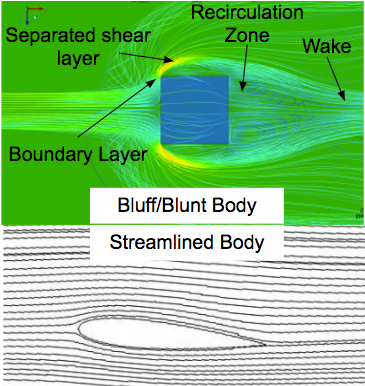
\includegraphics[width=0.45\textwidth]{Images/logan/bluntVSstreamline.png}
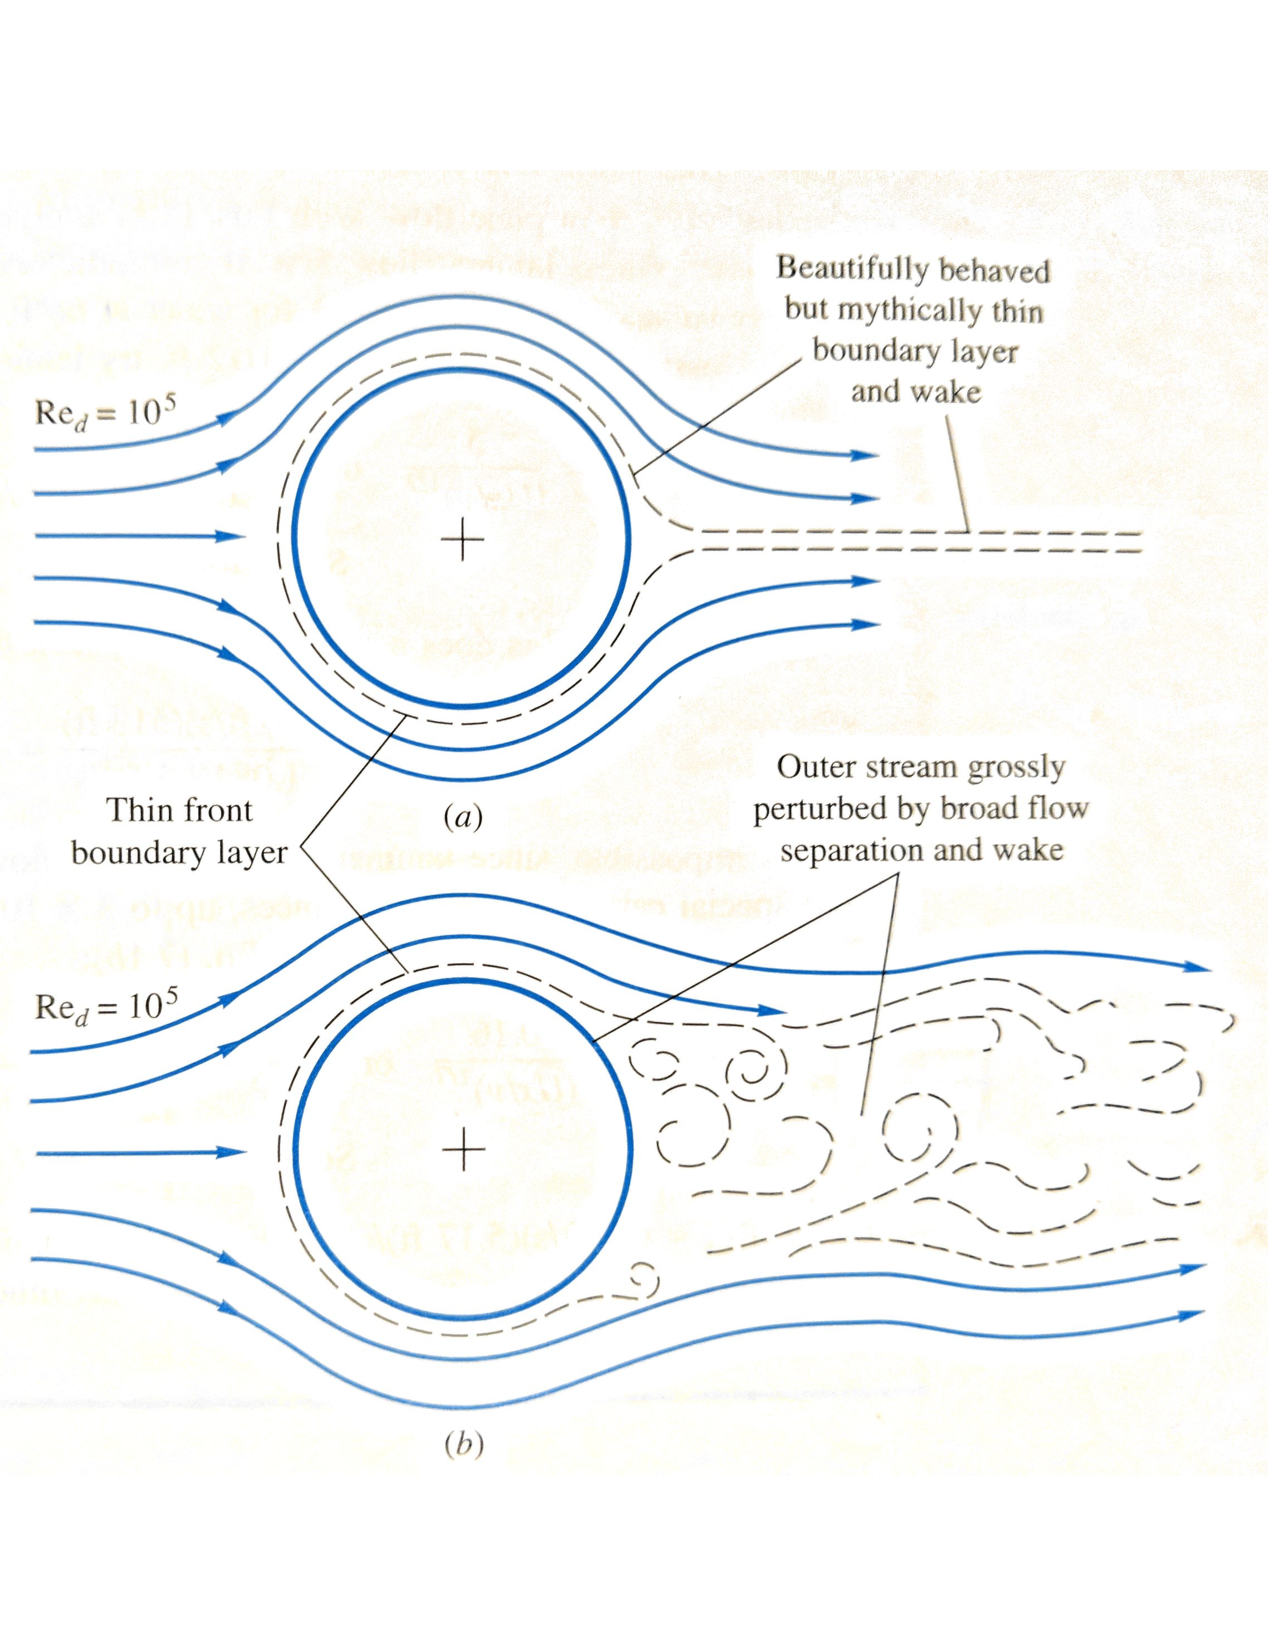
\includegraphics[width=0.49\textwidth]{Images/logan/white2011fluid_BluffBodyInviscidVSViscous.pdf}
\caption{ Demonstration of the flow differences between a bluff-body with massive separation \cite{richards2015modelling} and a streamlined body with primarily attached flow (left) and illustration of non-physical, inviscid flow over a bluff-body with no separation and realistic, viscous flow with massive separation (right) \cite{white2011fluid} }
\label{fig:bluffvsstreamlined}
\end{center}
\end{figure}
%%\vspace{-2em}










%%%%%%%%%%%%%%%%%%%%%%%%%%%%%%%%%%%%%%%%%%%%%%%%%%%%%%%%%%%%
%REAL WORLD APPLICATIONS

Bluff-body flow is applicable to a plethora of real-world applications.  Massively separated wakes are characterized by complex, unsteady, and sometime unstable turbulent phenomena, which can lead to design concerns throughout the fields of engineering. A few examples of bluff-body flow in engineering applications include wall-mounted cubes representative of a high-rise buildings \cite{elkhoury2016assessment}, bridge spans \cite{yuan2017investigation} as modeled in Fig~\ref{fig:tacomanarrowswake}, ground vehicles \cite{mendonca2002towards} like the passenger sedan shown in Fig~\ref{fig:carwake}, atmospheric reentry vehicles \cite{ross2013comprehensive} like the Orion wind tunnel model in Fig~\ref{fig:orionwakeandejectionseat}, humans in ejection seats and parachutes, both demonstrated in Fig~\ref{fig:orionwakeandejectionseat}, aircraft protuberances such as landing-gear trucks, space launch vehicles, and flame holders \cite{tanaka2013bluff} in combustors Fig~\ref{fig:flameholder}.

Bluff-bodies are common in civil engineering applications, where engineers might be concerned in predicting unsteady wind loading leading to structural resonance, which was a major design flaw for the Tacoma Narrows Bridge.  Fig~\ref{fig:tacomanarrowswake} demonstrates a model bridge span undergoing wake-induced vibration due to the vortex shedding caused by the gap in the center \cite{yuan2017investigation}.

%%% TACOMA NARROWS WAKE
%%\vspace{-2em}
\begin{figure}[htb]
% \begin{figure}[H]
\begin{center}
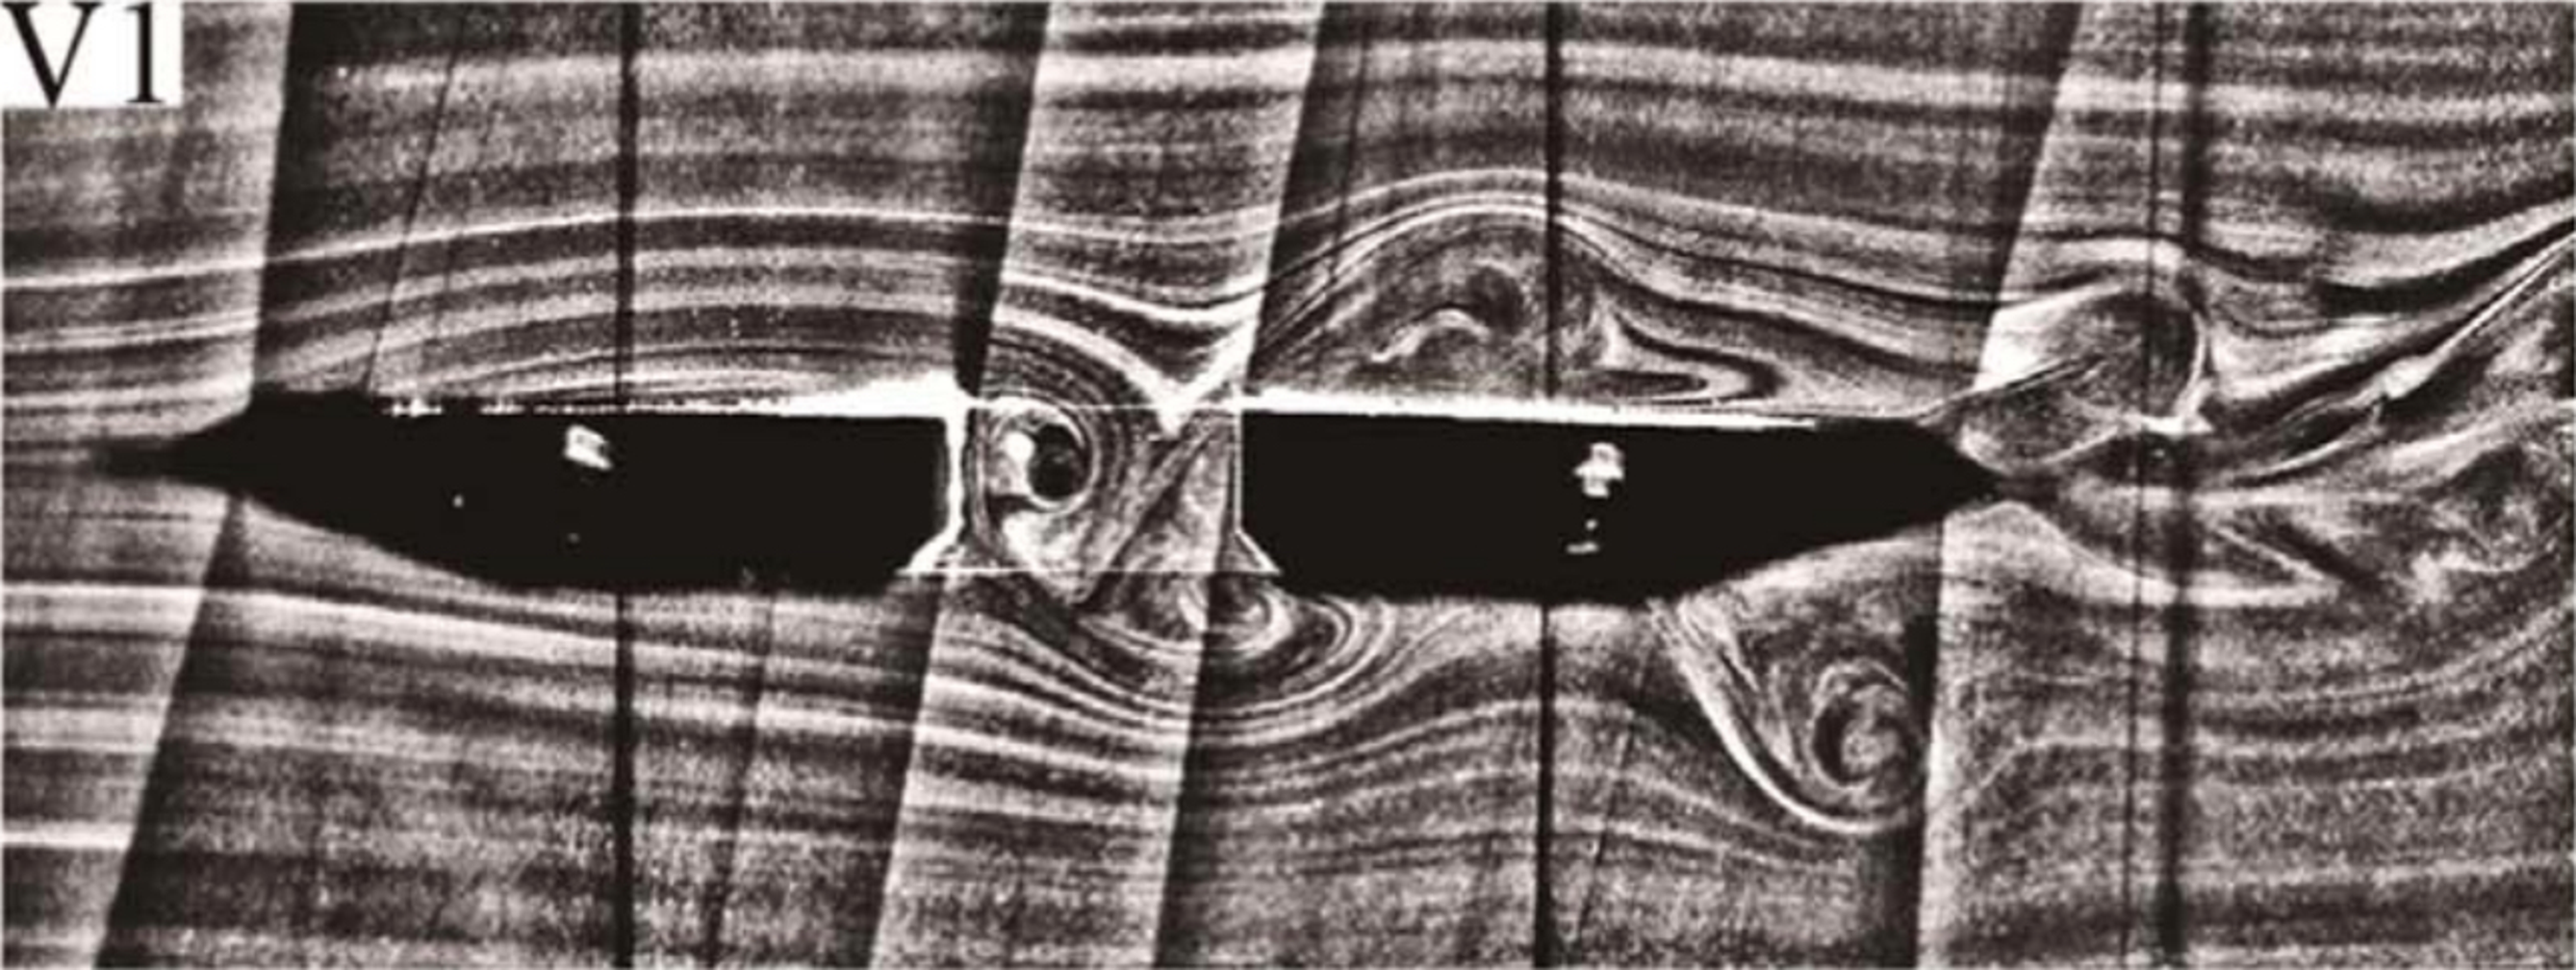
\includegraphics[width=0.7\textwidth]{Images/logan/yuan2017investigation_TacomaNarrowsWake.pdf}
\caption{ Instantaneous PIV flow field of bridge model similar to Tacoma Narrows bridge (Re=587) \cite{yuan2017investigation} }
\label{fig:tacomanarrowswake}
\end{center}
\end{figure}
%%\vspace{-2em}

Unsteady loading and buffeting can also be a potentially catastrophic bluff-body wake effect for mechanical and aerospace engineering applications.  The dynamic situation of a cockpit emergency egress system as depicted in Fig~\ref{fig:orionwakeandejectionseat} requires precise understanding of the unsteady forces on the ejection seat and human in order to mitigate any injuries the escaping pilot might experience.

%%% EJECTION SEAT and ORION WAKE
%%\vspace{-2em}
\begin{figure}[htb]
% \begin{figure}[H]
\begin{center}
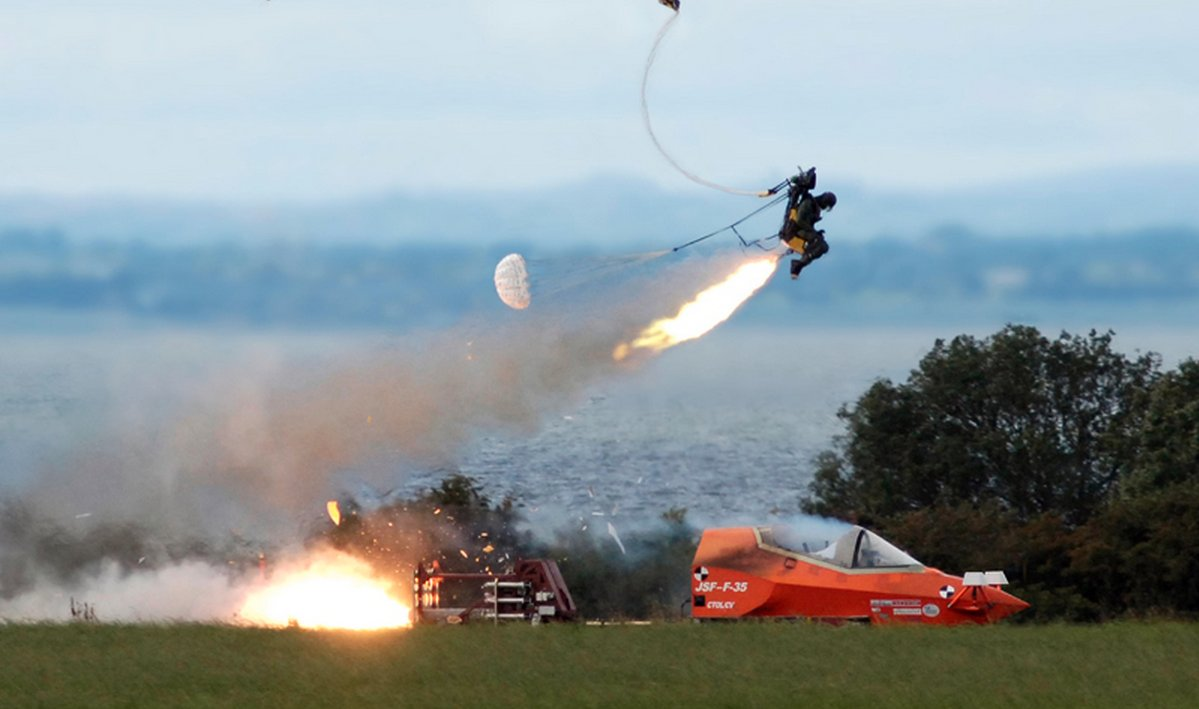
\includegraphics[width=0.48\textwidth]{Images/logan/martinbaker_EjectionSeat.jpg}
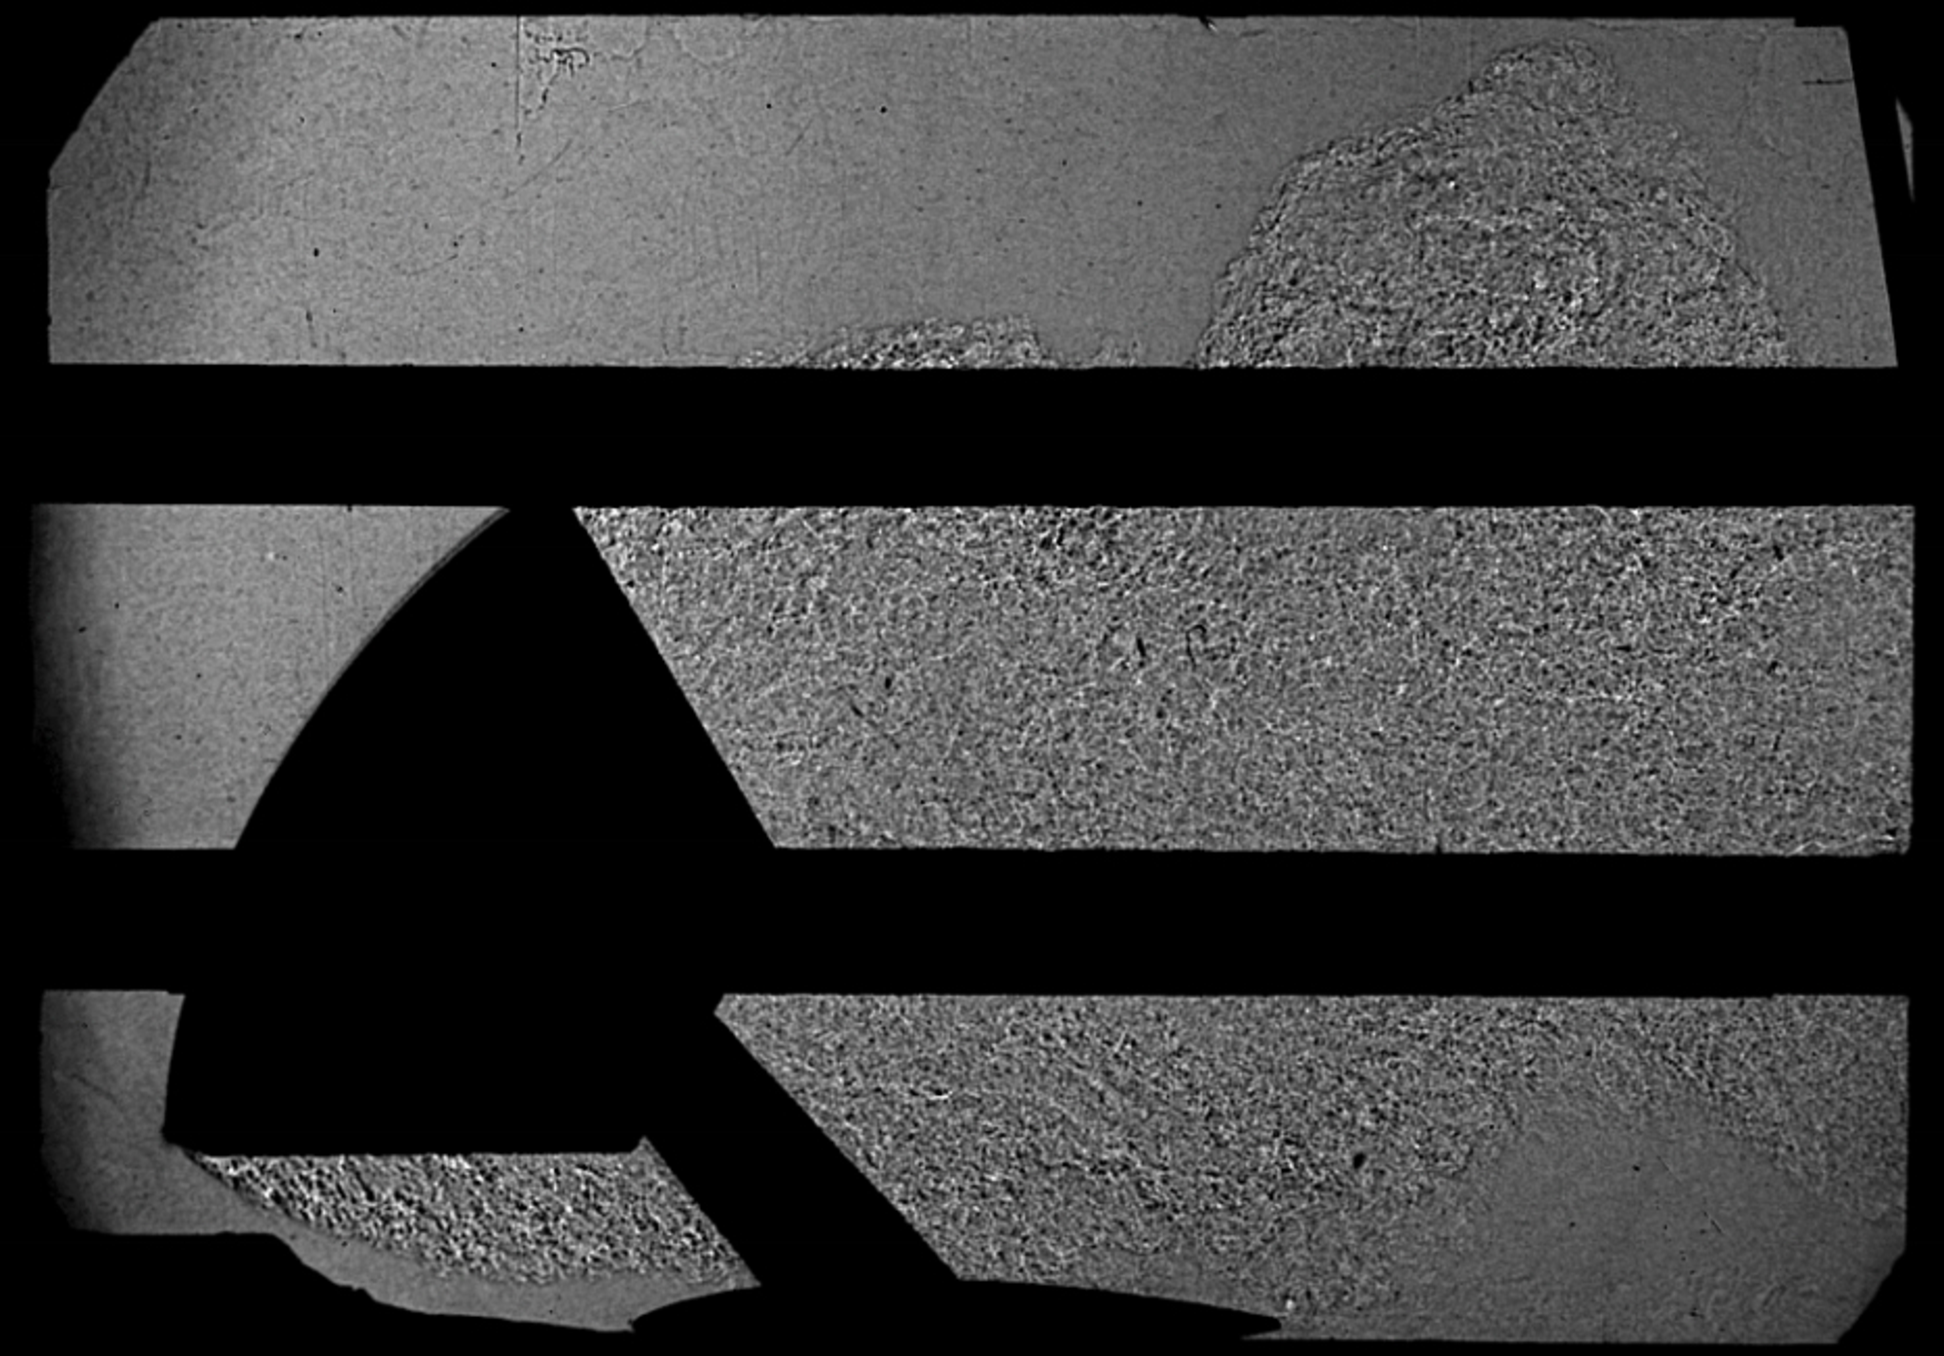
\includegraphics[width=0.41\textwidth]{Images/logan/ross2013comprehensive_CapsuleWakeShadowgraph.pdf}
\caption{ Left: Mk-16 ejection seat rocket sled test (Martin-Baker), Right: Shadowgraph wake of Orion capsule model ($M=0.3, \alpha=29.25^o, Re_D = 5.3\times10^6$) \cite{ross2013comprehensive}}
\label{fig:orionwakeandejectionseat}
\end{center}
\end{figure}
%%\vspace{-2em}

Dynamic stability can also be adversely affected by bluff-body wake behavior.  The drogue parachute in Fig~\ref{fig:orionwakeandejectionseat} and the model Orion capsule in Fig~\ref{fig:orionwakeandejectionseat} are both situations where dynamic instability of the bluff-body could lead to potentially fatal situations for the humans involved.

Acoustics can also be a design concern either due to unsteady loading as in the case of a launch vehicle or due to noise concerns or restrictions such as those for aircraft noise. Even passenger vehicles such as that shown in Fig~\ref{fig:carwake} can create a separated wake which could lead to acoustic disturbance of the passengers inside.

%%% CAR WAKE
%%\vspace{-2em}
\begin{figure}[htb]
% \begin{figure}[H]
\begin{center}
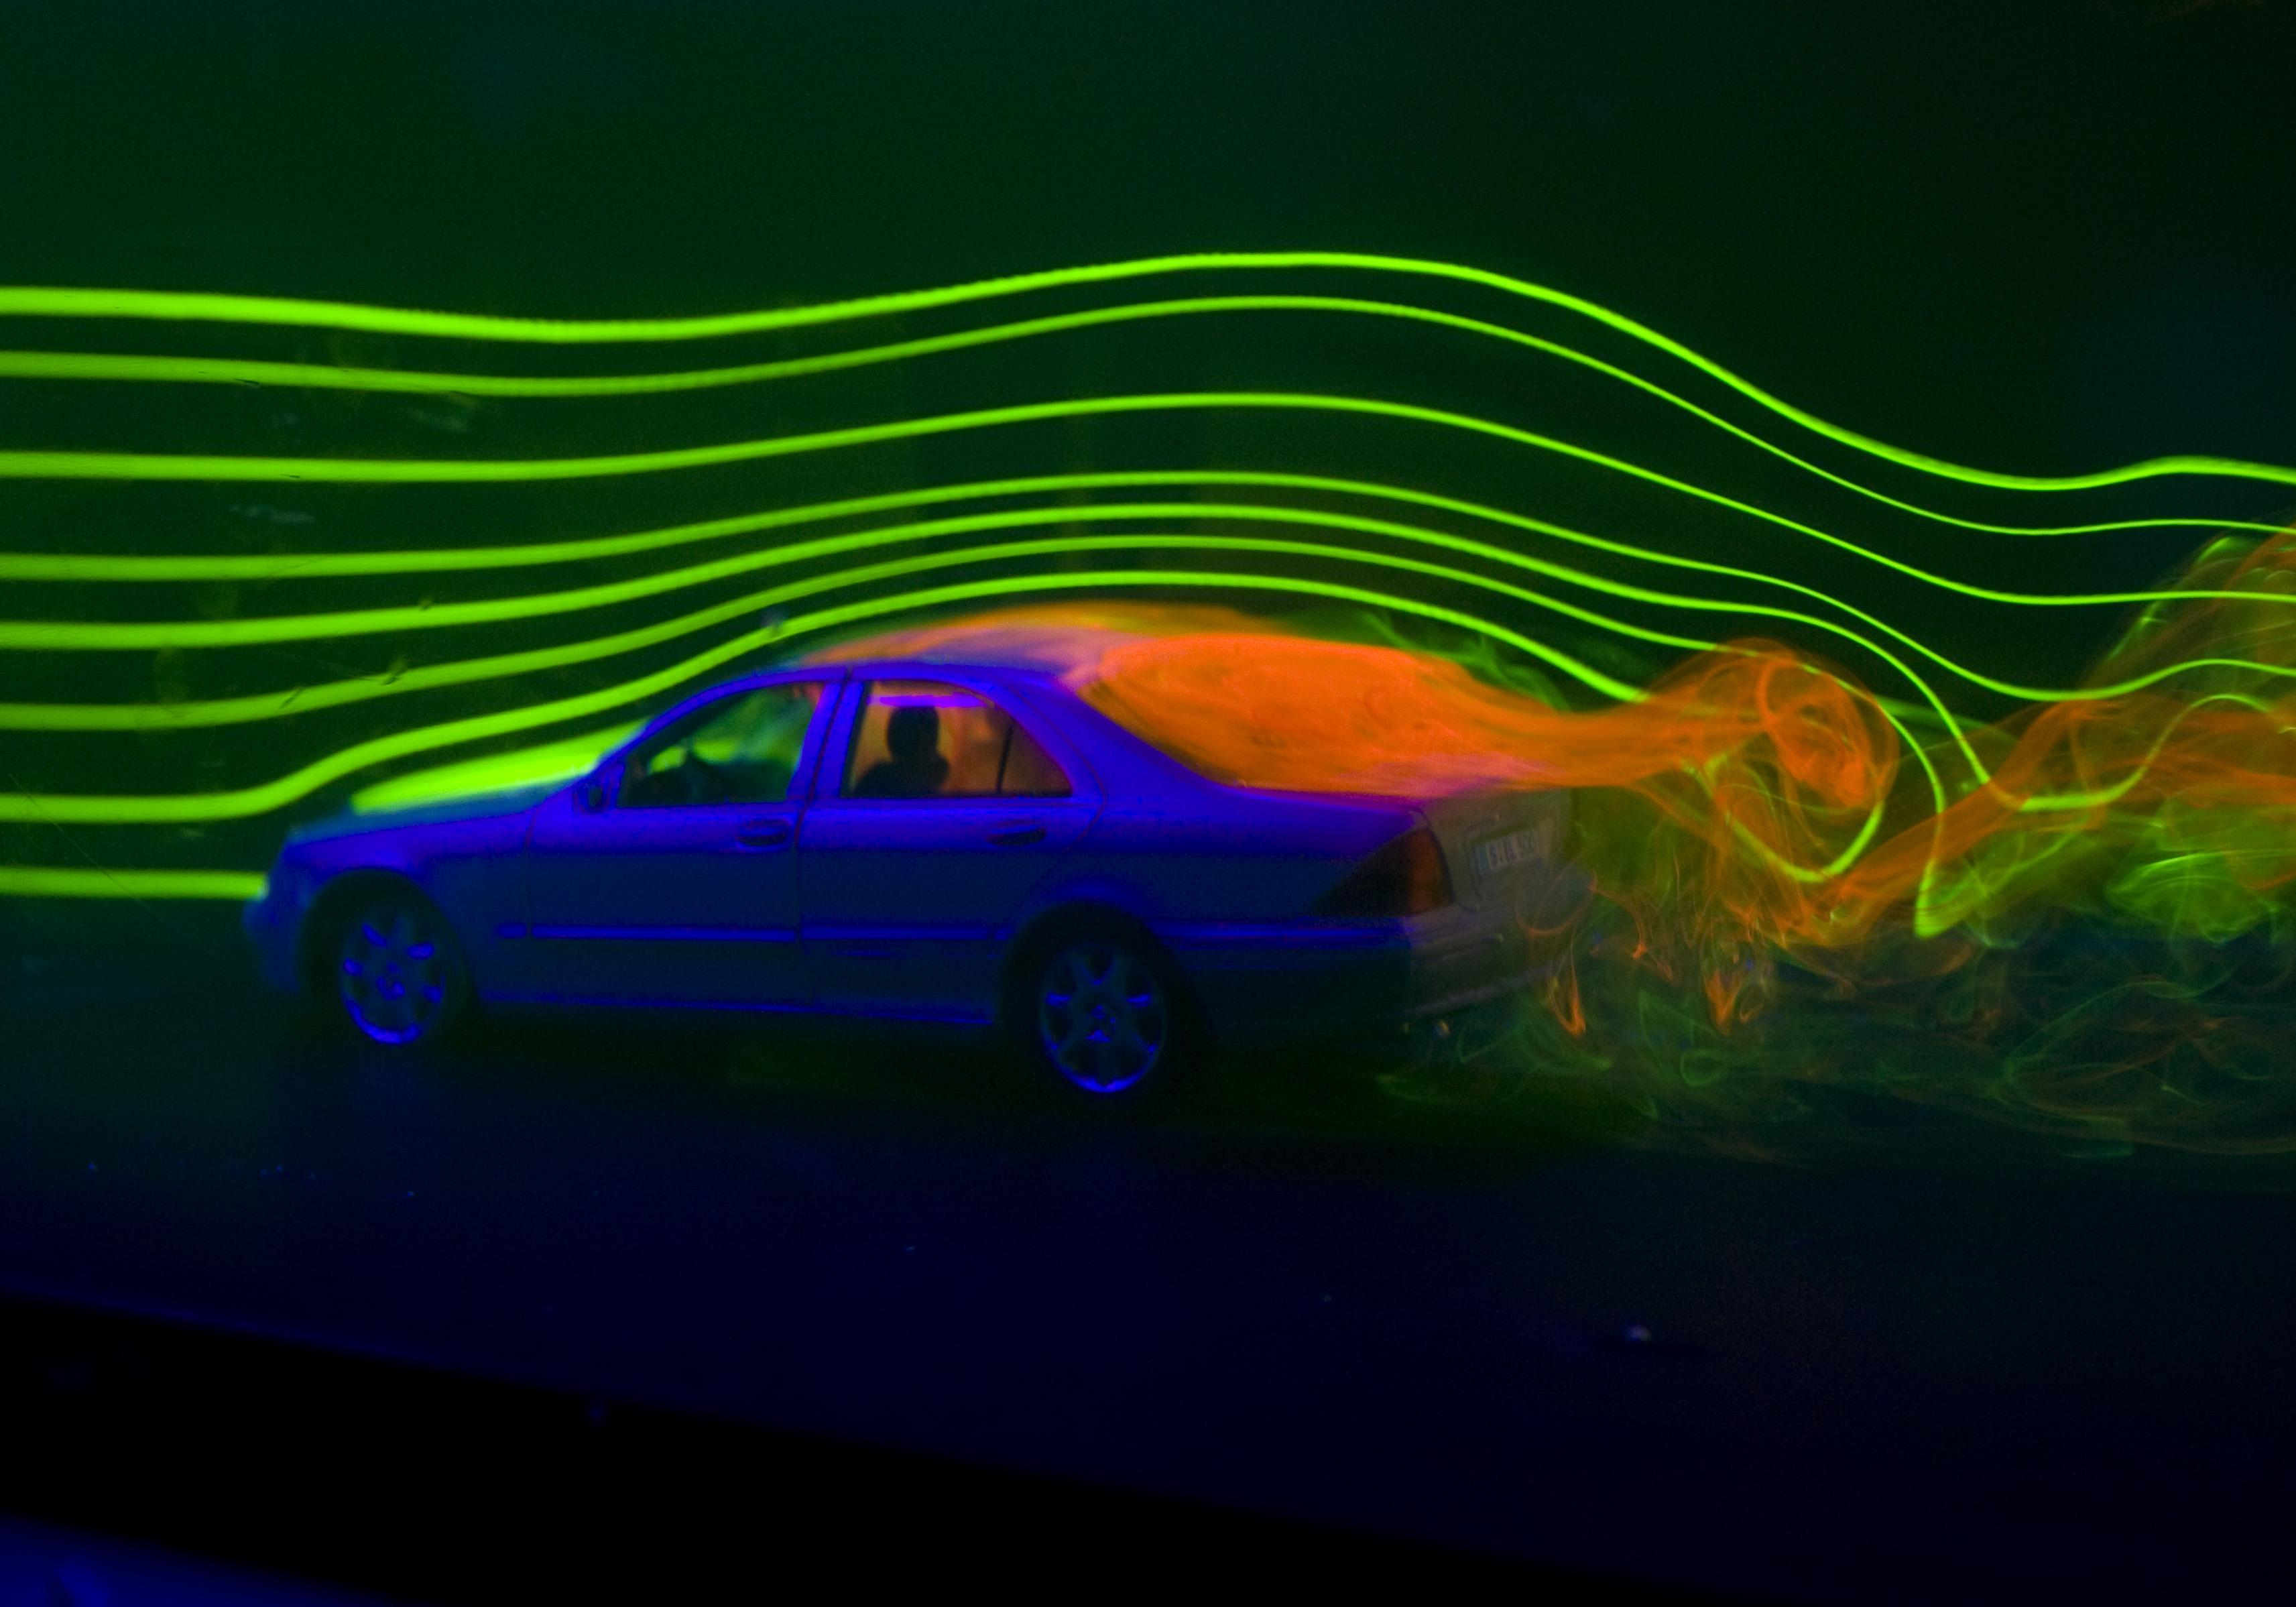
\includegraphics[width=0.5\textwidth]{Images/logan/james_CarWakePIV.jpg}
\caption{ Streamlines and separated flow over a car in a wind tunnel (NASA/Eric James) }
\label{fig:carwake}
\end{center}
\end{figure}
%%\vspace{-2em}

There are even applications for bluff-bodies outside the concepts of loading and acoustics. In industrial applications where a high-speed mixture must be ignited, it is necessary to both reduce the speed and mix the flow around an ignition source to allow a flame to stabilize. This effect can be created by placing a triangular bluff-body directly upstream of an ignitor such that its recirculation region entrains slower-moving mixture at the ignitor's location (Fig~\ref{fig:flameholder}) \cite{li2011large}.

%%% BLUFF BODY FLAME HOLDER
%%\vspace{-2em}
\begin{figure}[htb]
% \begin{figure}[H]
\begin{center}
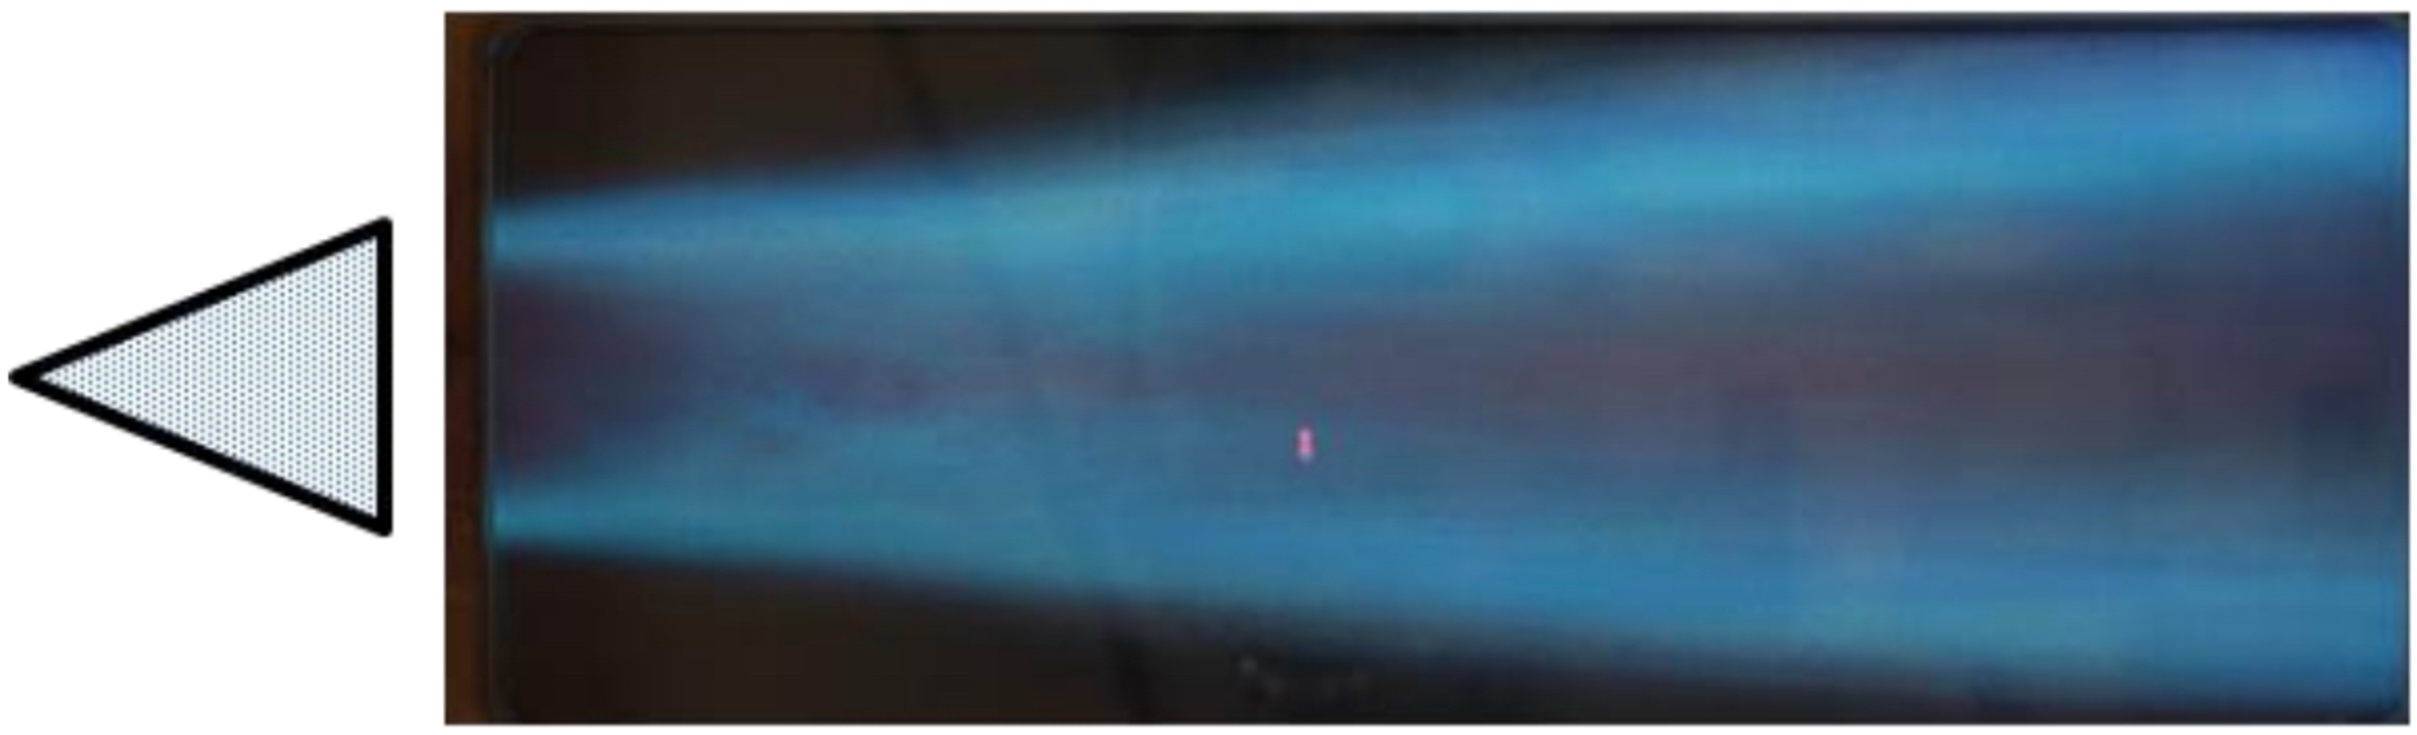
\includegraphics[width=0.7\textwidth]{Images/logan/tanaka2013bluff_FlameHolder.pdf}
\caption{ Image of a stabilized flame held in the wake of a bluff-body flame holder \cite{tanaka2013bluff} }
\label{fig:flameholder}
\end{center}
\end{figure}
%%\vspace{-2em}



The wakes of bluff-bodies are extremely complex, containing many scales of turbulent structures and can be highly unstable. These facts simultaneously impress upon the importance of understanding the effects of bluff-body flows for engineering applications and gives rise to long-term difficulties in modeling and observing bluff-body flow. The study presented in this article will attempt to connect the entire field of bluff-body fluid dynamics, archiving the fundamental concepts and historical approaches, assessing modern techniques of experimental and computational analysis, and discussing the challenges that remain.



% \emph{Big whorls have little whorls, which feed on their velocity, and little whorls have lesser whorls, and so on to viscosity (in the molecular sense).}
% Richardson (1922) \cite{richardson1922weather}







































%%%%%%%%%%%%%%%%%%%%%%%%%%%%%%%%%%%%%%%%%%%%%%%%%%%%%%%%%%%%%%%%%%%%%%%%
\section{Flow around a bluff body and transition}
%%%%%%%%%%%%%%%%%%%%%%%%%%%%%%%%%%%%%%%%%%%%%%%%%%%%%%%%%%%%%%%%%%%%%%%%

\begin{figure}[H]
\begin{center}
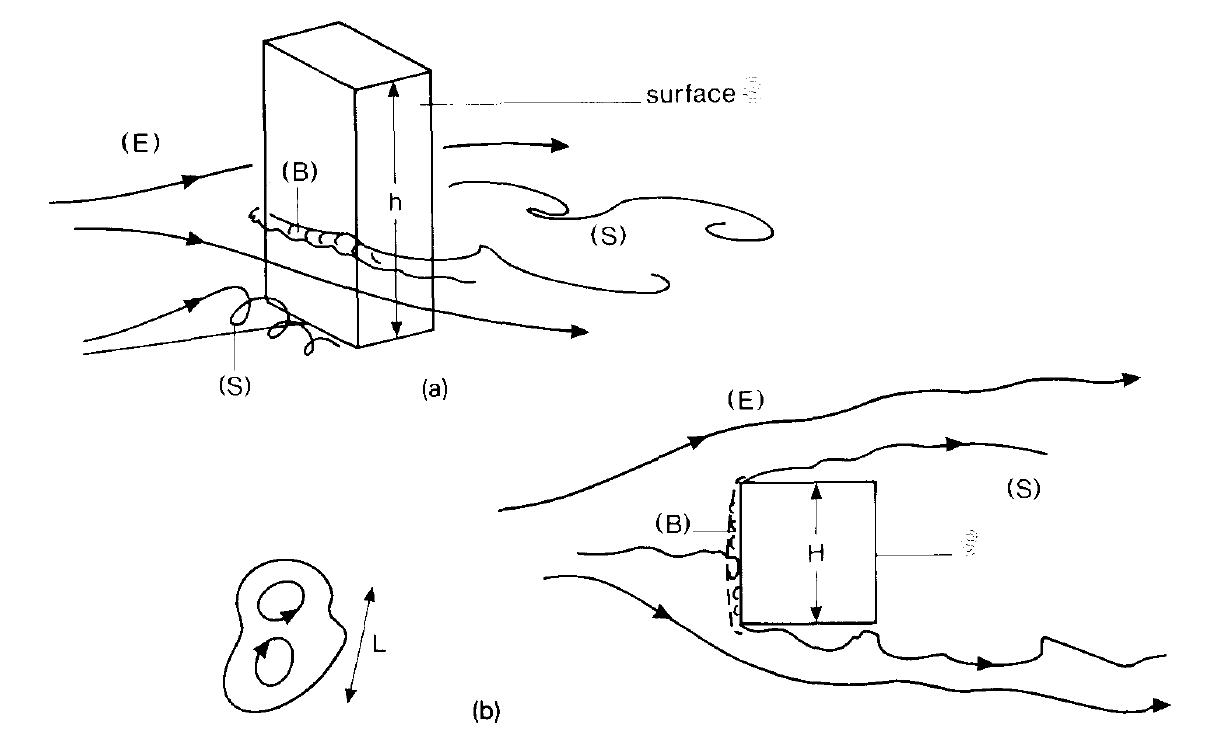
\includegraphics[width=0.7\textwidth]{Images/federico/Figure01}
\caption{ Regions of disturbed flow. Extracted from \cite{hunt1990} }
\label{fig:RegionsFlow}
\end{center}
\end{figure}

%%%%%%%%%%%%%%%%%%%%%%%%%%%%%%%%%%%%%%%%%%%%%%%%%%%%%%%%%%%%%%%%%%%%%%%%
\subsection{Steady laminar wake}

%%%%%%%%%%%%%%%%%%%%%%%%%%%%%%%%%%%%%%%%%%%%%%%%%%%%%%%%%%%%%%%%%%%%%%%%
\subsection{Periodic Laminar Regime}


\begin{figure}[H]
\begin{center}
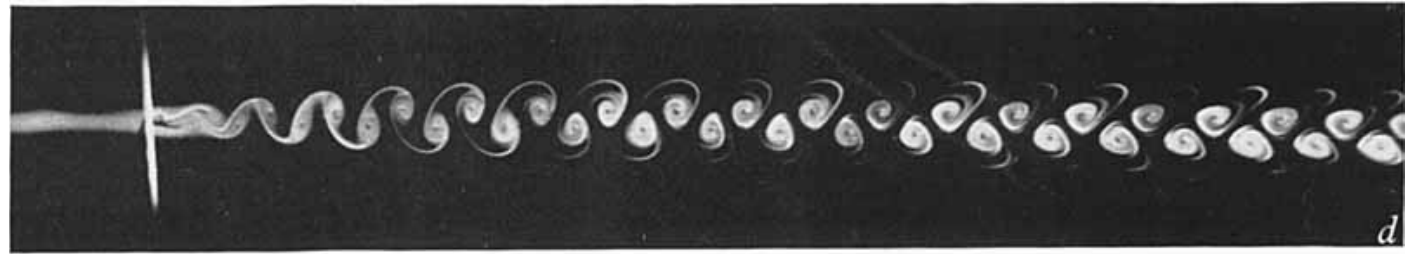
\includegraphics[width=1\textwidth]{Images/federico/Figure02}
\caption{Kárman-Bénard eddy street at \textbf{\textit{Re = 100}}. Extracted from \cite{Zdravkovich1968} }
\label{fig:Laminar}
\end{center}
\end{figure}

%%%%%%%%%%%%%%%%%%%%%%%%%%%%%%%%%%%%%%%%%%%%%%%%%%%%%%%%%%%%%%%%%%%%%%%%
\subsection{Transition in wake state}

\begin{figure}[H]
\begin{center}
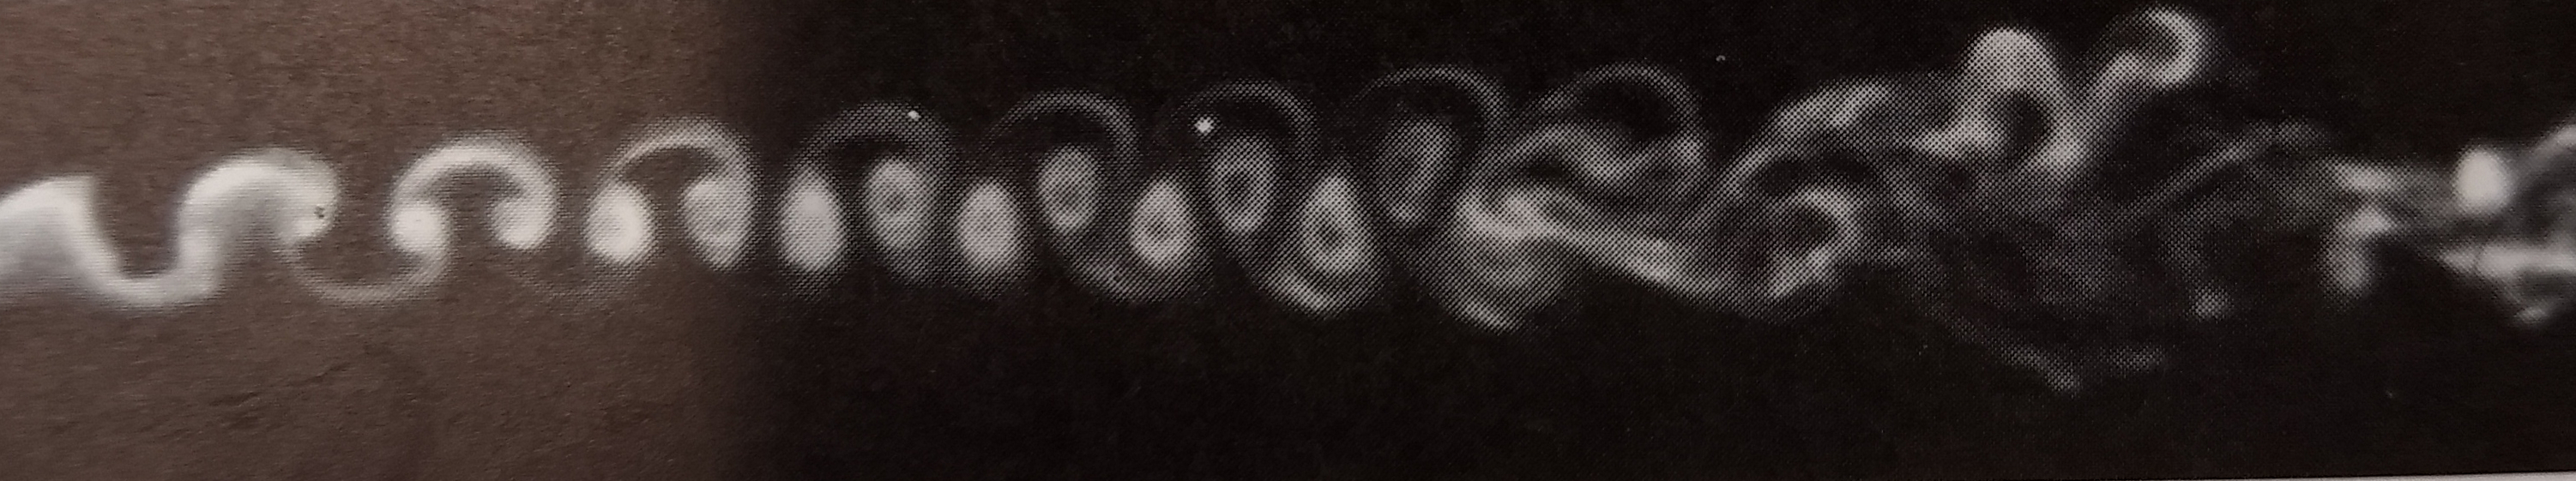
\includegraphics[width=1\textwidth]{Images/federico/Figure03}
\caption{Transition in wake at \textbf{\textit{Re = 190}}. Extracted from \cite{Zdravkovich1968} }
\label{fig:TrW1}
\end{center}
\end{figure}

\begin{figure}[H]
\begin{center}
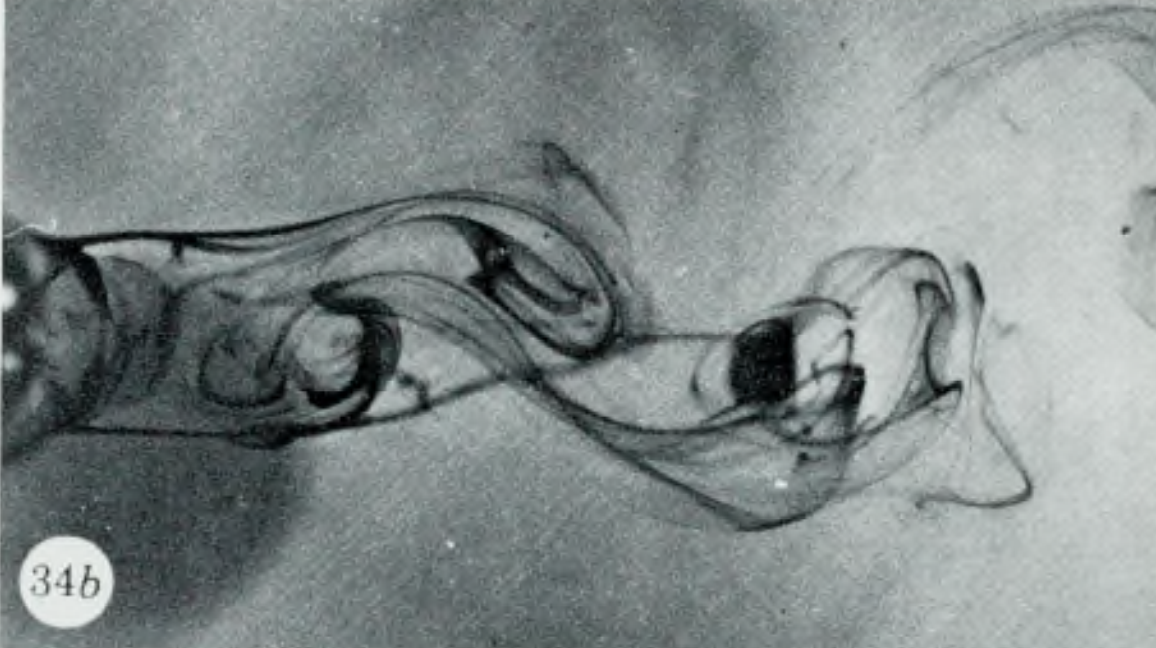
\includegraphics[width=0.5\textwidth]{Images/federico/Figure04}
\caption{Transition in wake at \textbf{\textit{Re = 344}}. Extracted from \cite{Gerrard1978} }
\label{fig:TrW2}
\end{center}
\end{figure}

%%%%%%%%%%%%%%%%%%%%%%%%%%%%%%%%%%%%%%%%%%%%%%%%%%%%%%%%%%%%%%%%%%%%%%%%
\subsection{Transition in shear layers state}

\begin{figure}[H]
\begin{center}
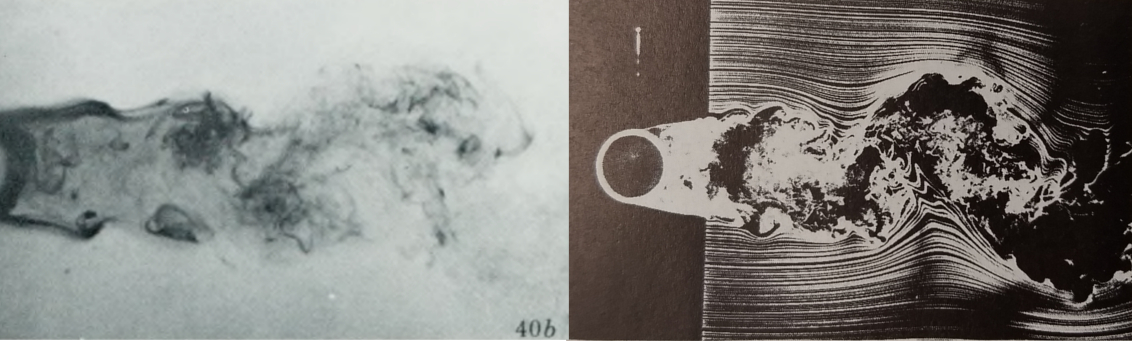
\includegraphics[width=1\textwidth]{Images/federico/Figure05}
\caption{Transition in free shear layer. Left: \textbf{\textit{Re = 1083}}. Extracted from \cite{Gerrard1978}. Right: \textbf{\textit{Re = 8000}}. Extracted from \cite{Zdravkovich1997}}
\label{fig:TrSL}
\end{center}
\end{figure}

%%%%%%%%%%%%%%%%%%%%%%%%%%%%%%%%%%%%%%%%%%%%%%%%%%%%%%%%%%%%%%%%%%%%%%%%
\subsection{Transition in boundary layer}


%%%%%%%%%%%%%%%%%%%%%%%%%%%%%%%%%%%%%%%%%%%%%%%%%%%%%%%%%%%%%%%%%%%%%%%%
\subsection{Fully turbulent state}








%%%%%%%%%%%%%%%%%%%%%%%%%%%%%%%%%%%%%%%%%%%%%%%%%%%%%%%%%%%%%%%%%%%%%%%%
\section{Free stream turbulence and non-uniform free stream}
%%%%%%%%%%%%%%%%%%%%%%%%%%%%%%%%%%%%%%%%%%%%%%%%%%%%%%%%%%%%%%%%%%%%%%%%










%%%%%%%%%%%%%%%%%%%%%%%%%%%%%%%%%%%%%%%%%%%%%%%%%%%%%%%%%%%%%%%%%%%%%%%%
\section{Experimental Methods And Results} \label{sec:experimentalmethods}
%%%%%%%%%%%%%%%%%%%%%%%%%%%%%%%%%%%%%%%%%%%%%%%%%%%%%%%%%%%%%%%%%%%%%%%%

\textcolor{red}{\emph{FZ}}

\begin{itemize}
    \item Historical Study
    \item Experimental techniques
    \begin{itemize}
        \item ballistic range?
    \end{itemize}
    \item Applications
    \begin{itemize}
        \item Simple cases: cylinder/sphere
        \begin{itemize}
            \item Drag vs Re?
            \item Wake velocity profiles?
            \item Wake structure?
        \end{itemize}
        \item Sharp vs bluff: sphere vs cube
        \item Complex cases: capsule/building
    \end{itemize}
\end{itemize}






















%%%%%%%%%%%%%%%%%%%%%%%%%%%%%%%%%%%%%%%%%%%%%%%%%%%%%%%%%%%%%%%%%%%%%%%%
\section{Computational Methods and Results} \label{sec:computationalmethods}
%%%%%%%%%%%%%%%%%%%%%%%%%%%%%%%%%%%%%%%%%%%%%%%%%%%%%%%%%%%%%%%%%%%%%%%%

Due to the highly complex nature of bluff-body wake separation and behavior, the primary realistic method of simulation for these flows is discrete solution of the Navier-Stokes equations (Eqn~\ref{eqn:navierstokes}) or Computational Fluid Dynamics (CFD). Analytic, inviscid formulations such as potential flow methods yield the non-physical results depicted in the top image of Fig~\ref{fig:bluffvsstreamlined}, where there is separation or corresponding base pressure, making this fictional flow a non-bluff-body. The same deficiencies apply to numeric, inviscid formulations, such as panel method or Euler's equation. Within the field of CFD, there is a diverse set of techniques for handling the simulation of turbulence, and the detailed description of each of these is beyond the scope of this study. Instead, the key concept of each method relevant to bluff-body flow will be listed here to provide the basis for the comparisons to follow.


%%%%%%%%%%%%%%%%%%%%%%%%%%%%%%%%%%%%%%%%%%%%%%%%%%%%%%%%%%%%%%%%%%%%%%%%
\subsection{Turbulence Modeling Overview} \label{subsec:turbulencemodeling}

 Discrete solution of the full Navier-Stokes equations is referred to as Direct Numeric Simulation (DNS). The incompressible form of the continuity and momentum equations for this formulation are provided in Eqn~\ref{eqn:navierstokes}. No turbulence modeling is required for this simulation, so results will be as realistic as the domain discretization and continuum, Newtonian fluid constraints allow. The disadvantage of DNS lies in the requirement that all scales of turbulence must be resolved within the domain to achieve realistic results, which makes simulation of the majority of flows infeasible with the current state of computational technology.

\begin{equation}
\label{eqn:navierstokes}
\begin{split}
\vec{\nabla}\vec{V} &= 0 \\
\rho \dfrac{D \vec{V}}{D t}
    &= \rho\vec{g} - \vec{\nabla} P + \mu \vec{\nabla}^2 \vec{V}
\end{split}
\end{equation}

The Navier-Stokes equations can be reduced to a form that is solvable by todays standards by separating them in to mean and fluctuation components via the process of Reynolds decomposition. This results in the Reynolds-Average Navier-Stokes (RANS) equations of which the incompressible momentum equation is provided for example in Eqn~\ref{eqn:rans}.



\begin{equation}
\label{eqn:rans}
\rho \dfrac{D \overline{\vec{V}}}{D t}
    = \rho\vec{g} - \vec{\nabla} \overline{P}
    + \mu \vec{\nabla}^2 \overline{\vec{V}}
    - \rho \dfrac{\partial}{\partial x_j} \left( \overline{u'_i u'_j} \right)
\end{equation}

\noindent where the overbar represents the time average and the vertical tick represents a perturbation quantity. Unfortunately, the infamous turbulence closure problem requires that some relation must be derived for the additional unknown ``Reynolds stress'' term $\rho \overline{u'_i u'_j}$. Turbulence models allow the estimation of this term and the closure of the RANS equations to notable success, but inherent inaccuracy is introduced by the nature of modeling.

A slight variation of RANS is Unsteady RANS (URANS), which is a time-accurate method that requires all grid cells to be fixed to the same global time step.  This allows URANS to capture unsteady behavior of the mean flow.

In recent years, the advantages of DNS in resolving fine turbulent behavior have been brought into use through the compromising strategy of Large Eddy Simulation (LES), where turbulent structures that are large enough to be resolved on the chosen computational grid are solved with DNS, and smaller turbulent scales are solved with a turbulence model called a Subgrid-Scale (SGS) model. This methodology results in much higher fidelity turbulence spectra and unsteady behavior but comes at the cost of more computational time required.

This method was enhanced by Spalart to operate with RANS as the Subgrid Scale Model, effectively combing the two methods into a hybrid RANS/LES method coined Detached Eddy Simulation (DES) \cite{spalart2009detachededdy}.

Finally, Scale Adaptive Simulation (SAS) is a RANS-like method developed by Menter \cite{menter2005scaleadaptive} that uses a dynamic von Karman length-scale in its turbulence model, which allows the resolution of the full turbulent spectrum and results in LES-like results.











%%%%%%%%%%%%%%%%%%%%%%%%%%%%%%%%%%%%%%%%%%%%%%%%%%%%%%%%%%%%%%%%%%%%%%%%
\subsection{Initial Methodology Comparisons for a Circular Cylinder} \label{subsec:initialcompare}

The fundamental differences between the CFD methodologies previously described in Section~\ref{subsec:turbulencemodeling} can result in noticeable variations in simulation results; especially for massively separated wakes. A first look at these differences is offered in Fig~\ref{fig:cylinderturbmodels}, which is a comparison of flow over a circular cylinder calculated using various RANS and DES methods from Spalart and Travin \cite{spalart2009detachededdy} and comparable SAS cases from Menter \cite{menter2005scaleadaptive}. The circular cylinder is arguably the simplest bluff-body shape and therefore offers a relatively unbiased platform upon which to compare these different solvers.

In this instance, we are observing simulations for a diameter-based Reynolds number of $Re_D = 5 \times 10^4$, which corresponds to laminar separation, and we are comparing the time-averaged result for drag coefficient $C_d$ from each simulation to the range of instantaneous $C_d=1.15-1.25$ observed in experiment at a similar Reynolds number \cite{travin2000detachededdy}.

The simplest of all of these models is the steady RANS case (a), where the wake vorticity isocontours demonstrate that only the two-dimensional separated shear layer is predicted. This very low-fidelity wake results in a correspondingly inaccurate $C_d$ compared to the wind tunnel range. RANS simulations can be significantly improved, however, by modeling time-accurate changes in the mean and allowing three-dimensional flow effects to develop, as is the case for 3D URANS.  In this simulation, the flow is significantly more realistic than steady RANS, though much of the three-dimensionality is still suppressed \cite{spalart2009detachededdy}.  Averaging and integration of this wake behavior results in a $C_d$ that is just within the upper range of the wind tunnel values, which is a significant improvement upon steady RANS.

Even higher-fidelity results may be obtained from LES-based methods such as DES, for which three cases are shown in Fig~\ref{fig:cylinderturbmodels}. For all three cases, it is obvious that the application of DNS to the larger turbulence scales results in a more three-dimensional and life-like simulation of turbulent wake effects. This improvement in modeling can be useful for engineering design cases that require unsteady loading or acoustic profile data. The time-averaged $C_d$ values for each DES case, however, remain on the fringes of the experimental range, suggesting that the increased computational cost of DES may not always be compensated for by higher accuracy in time-averaged results. Still, it is important to note that these comparisons are highly dependent on the method and window of averaging and a single metric such as $C_d$ is insufficient on its own to determine the superiority of a CFD method \cite{travin2000detachededdy}. Further comparison of the capabilities of RANS and LES-like methods will be made in Section~\ref{subsec:desvsrans}.

The three DES results can also be used to illustrate uncertainties in the method due to discretization and turbulence modeling. The DES-SA (Spalart-Allmaras) cases demonstrate that grid refinement in the LES-regions allows resolution of fine turbulent scales and can significantly alter the time-averaged results. The comparison of the SA and Shear-Stress Transport (SST) RANS models demonstrates that the choice of RANS model has little effect on the LES-regions of the DES solution, but can noticeably influence the separation prediction in the RANS-regions.

Lastly, SAS simulations for a similar circular cylinder with $Re_D=3.6 \times 10^6$ are shown in the bottom of Fig~\ref{fig:cylinderturbmodels}, with the pure URANS case on the left and the dynamic length-scale turbulence model functionality on the right \cite{menter2005scaleadaptive}. Qualitative comparison shows that SAS can produce bluff-body flow features that are quite comparable to DES without any direct simulation. A more detailed comparison of accuracy and computational cost of these two methods can be found in Section~\ref{subsec:desvssas}.


%%% CYLINDER WITH VARIOUS TYPES OF NUMERICAL MODELING
%%\vspace{-2em}
% \begin{figure}[htb]
\begin{figure}[H]
\begin{center}
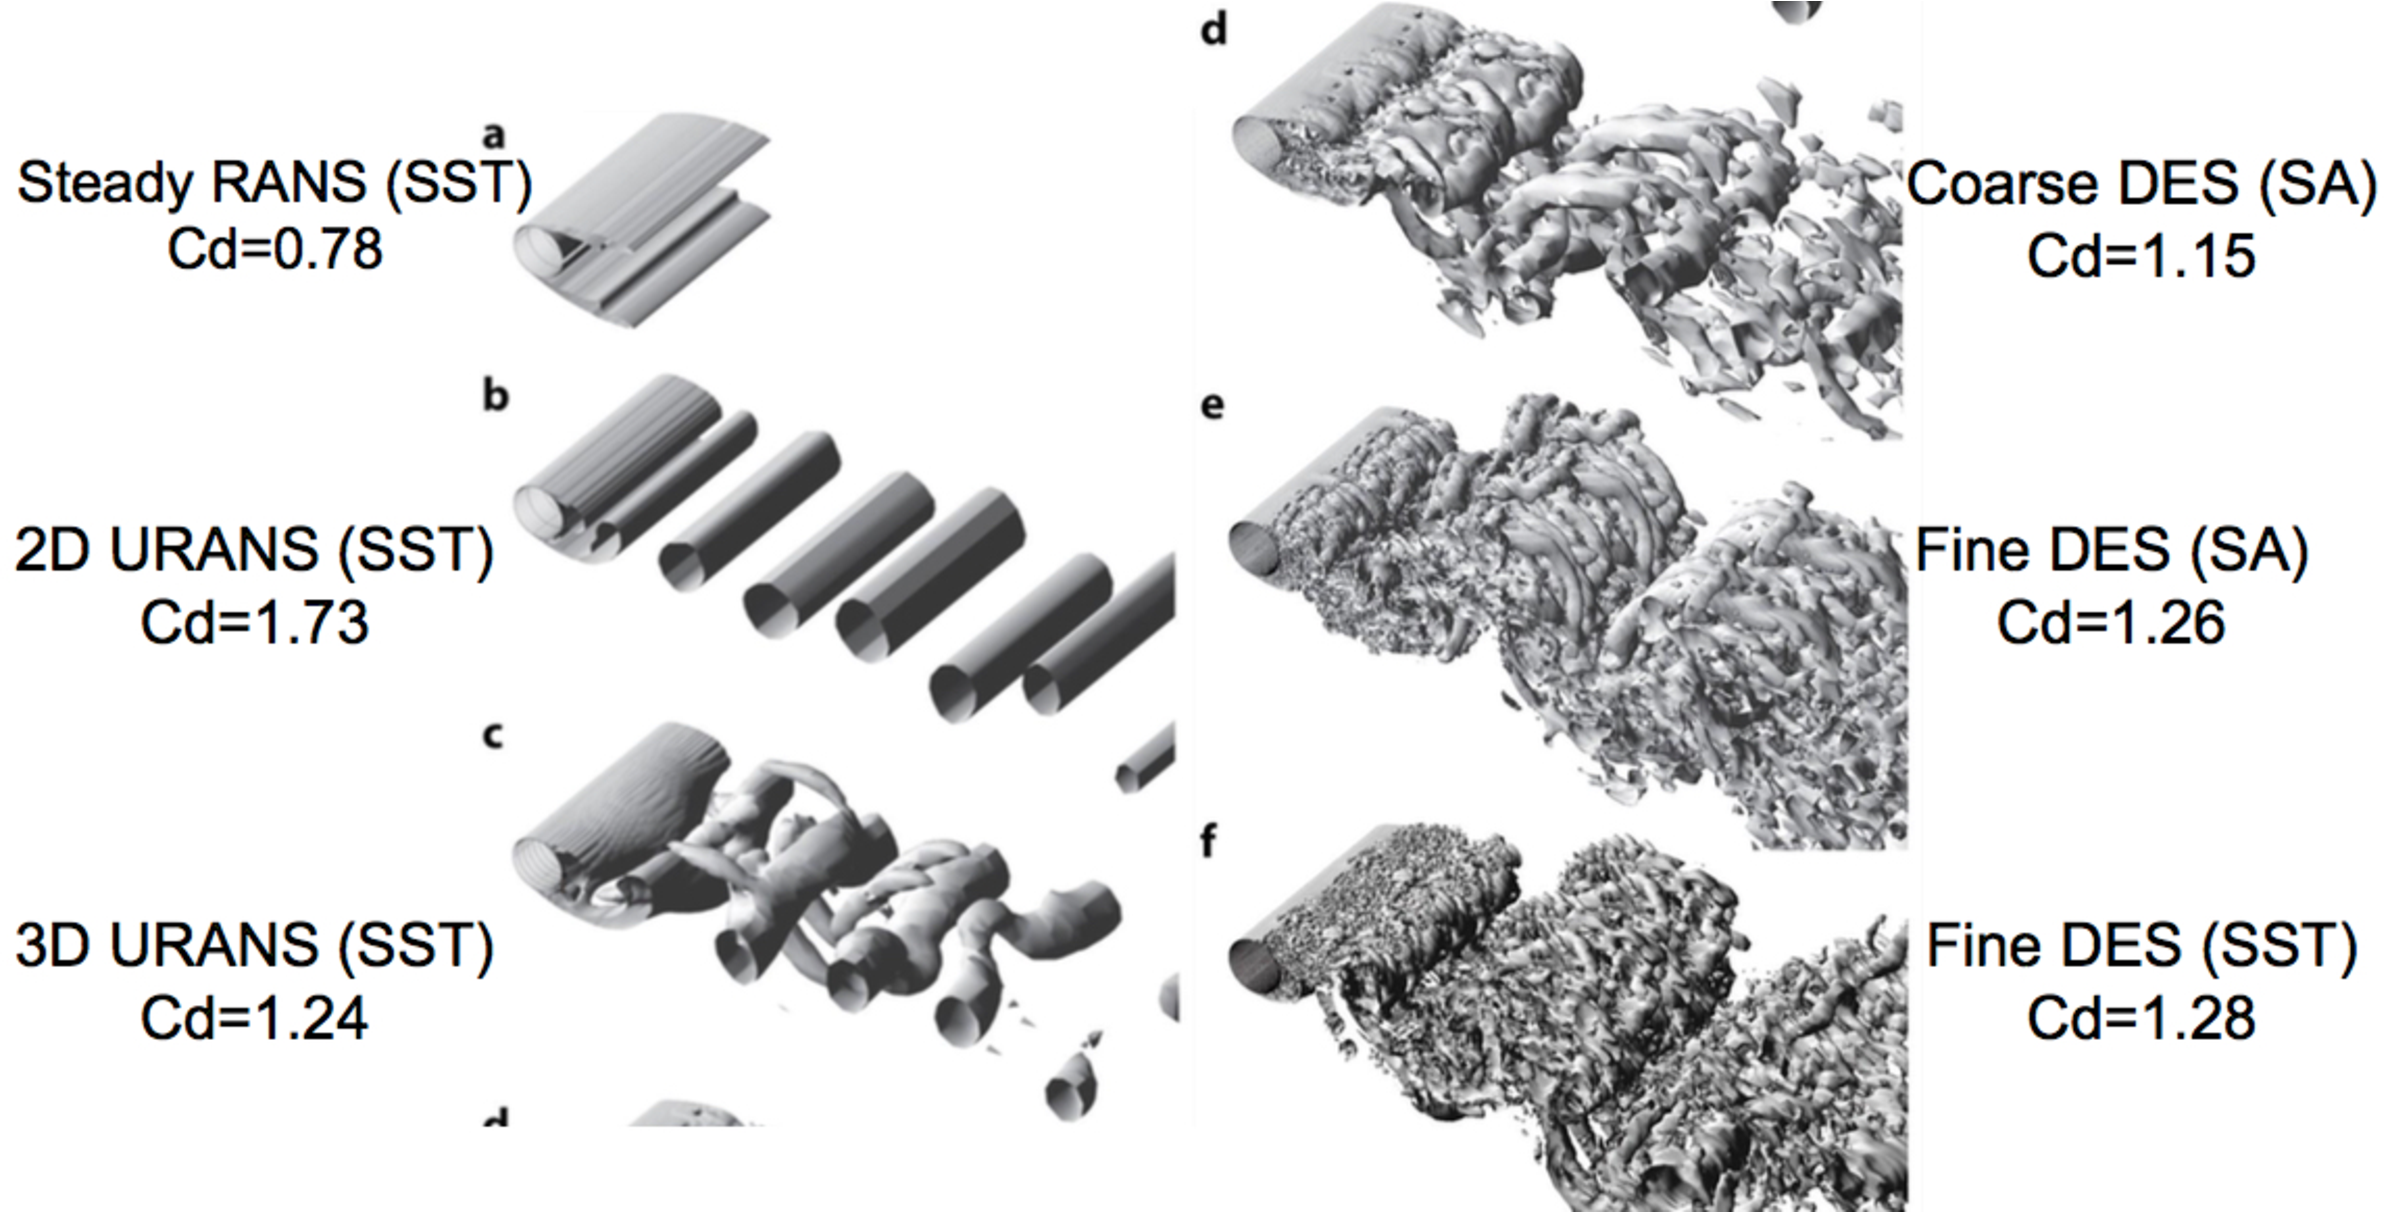
\includegraphics[width=1.0\textwidth]{Images/logan/spalart2009detachededdy_cylindersCD.pdf}
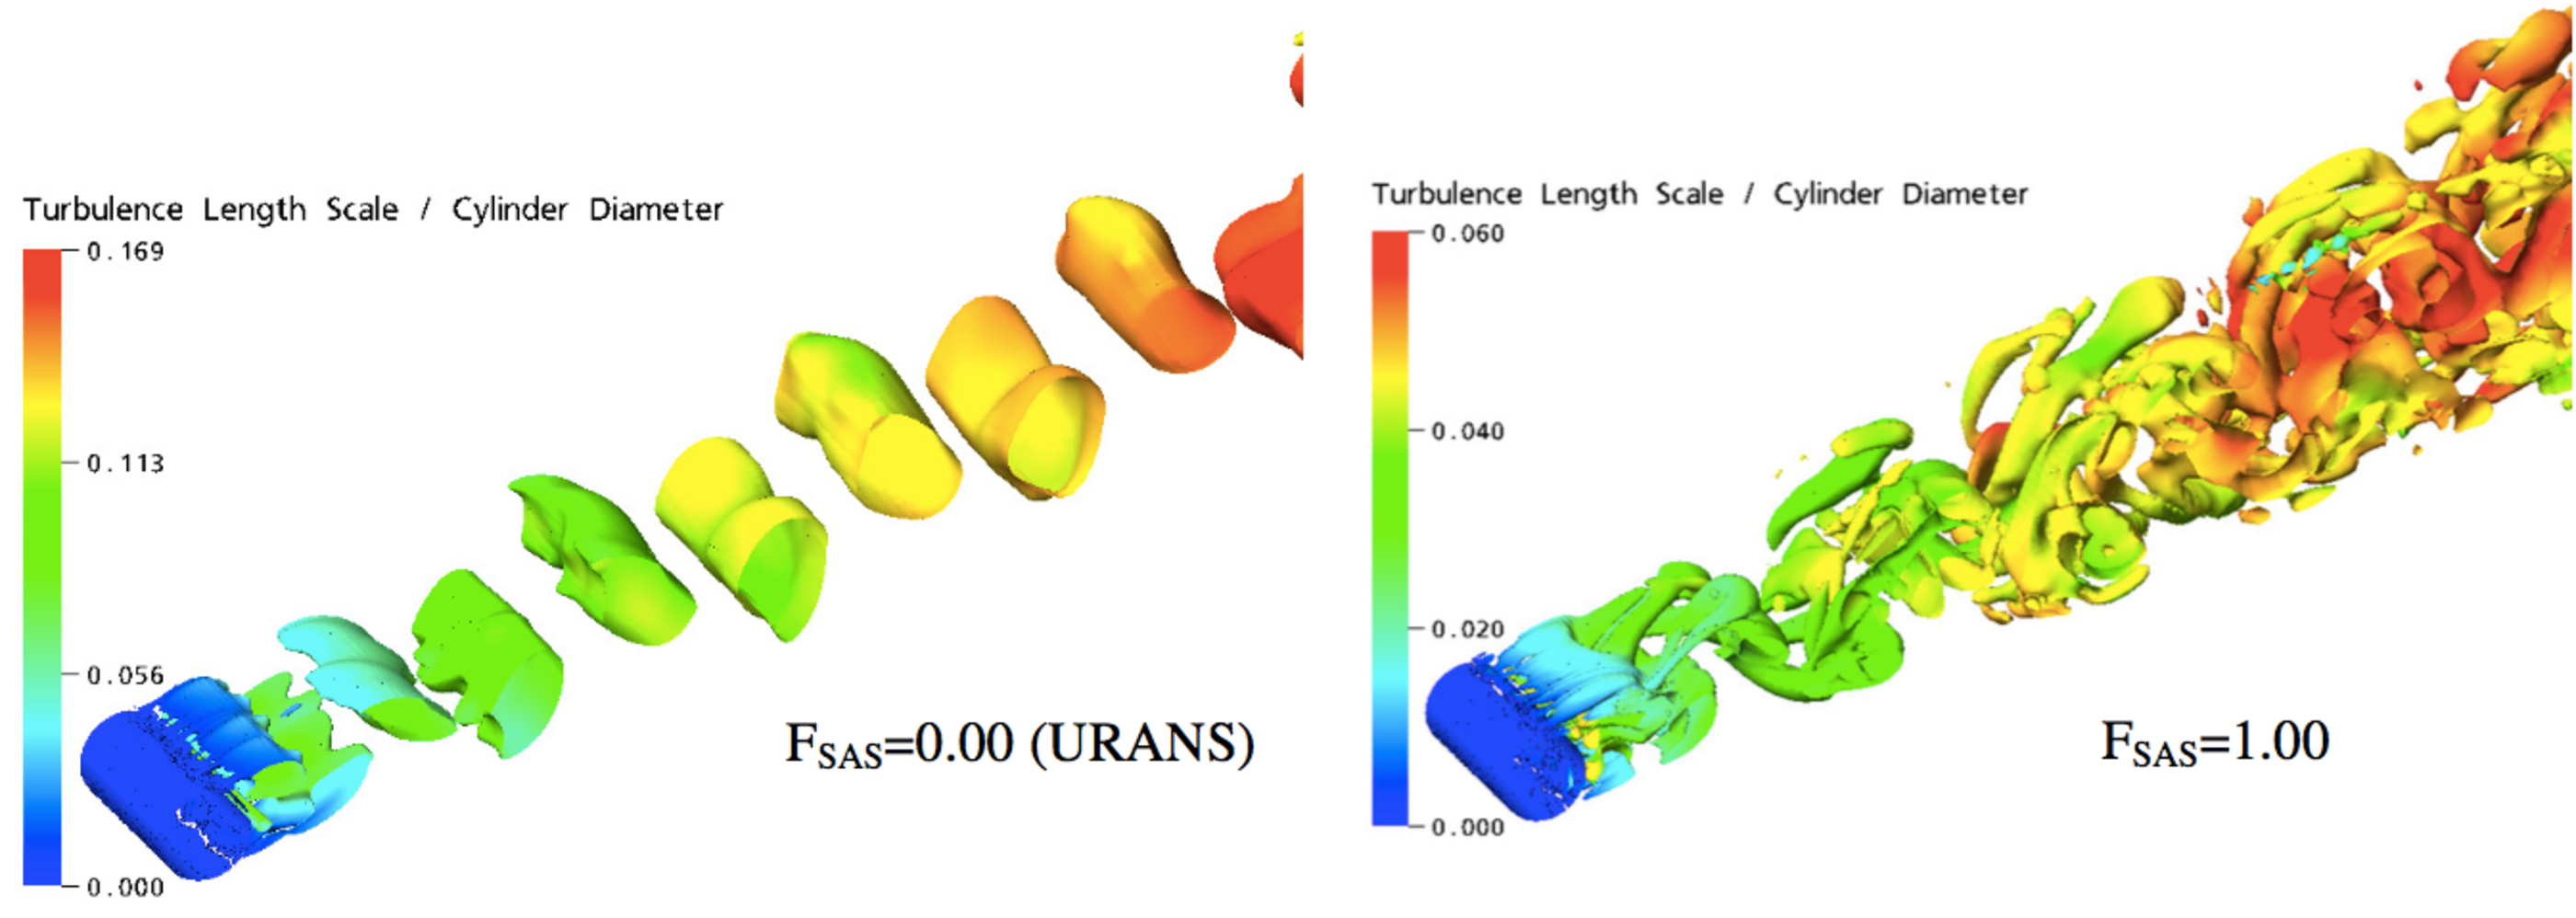
\includegraphics[width=0.65\textwidth]{Images/logan/menter2005scaleadaptive_cylinderwake.pdf}
\caption{ Comparison of wind tunnel test of a circular cylinder with drag fluctuating coefficient ranging from $C_d=1.15-1.25$ compared with time-averaged $C_d$ values from simulations using RANS (a), 2D URANS (b), 3D URANS (c), DES-SA on a coarse grid (d), DES-SA on a fine grid (f), and DES-SST on a fine grid (e) \cite{spalart2009detachededdy} in black and white and SAS simulations with null (left) and finite (right) adjustable length-scales in color \cite{menter2005scaleadaptive}. Visualizations are isocontours of vorticity }
\label{fig:cylinderturbmodels}
\end{center}
\end{figure}
%%\vspace{-2em}










%%%%%%%%%%%%%%%%%%%%%%%%%%%%%%%%%%%%%%%%%%%%%%%%%%%%%%%%%%%%%%%%%%%%%%%%
\subsection{Comparison of RANS and LES/DES Methodologies for Bluff-Bodies} \label{subsec:desvsrans}

Though Section~\ref{subsec:initialcompare} demonstrates that higher-fidelity CFD methodologies like LES are undoubtedly capable of more realistic unsteady bluff-body simulation than RANS methods, the ambiguity of the accuracy time-averaged results of each method calls for further comparison of the strengths and weaknesses of URANS and LES/DES in predicting time-averaged quantities for bluff-body flows.

First, URANS will be compared directly to LES in the study by Catalano et al. (2003) \cite{catalano2003numerical} of a circular cylinder at a relatively high Reynolds number of $Re_D = 1.0 \times 10^6$. A qualitative flow comparison of the two solutions in Fig~\ref{fig:cylinderransvslesflow} demonstrates that there is a obvious difference in both the instantaneous and time-averaged flow behavior between the two methods, which is consistent with the discussion in Section~\ref{subsec:initialcompare}.



%%% LES VS RANS CYLINDER FLOW
%%\vspace{-2em}
% \begin{figure}[htb]
\begin{figure}[H]
\begin{center}
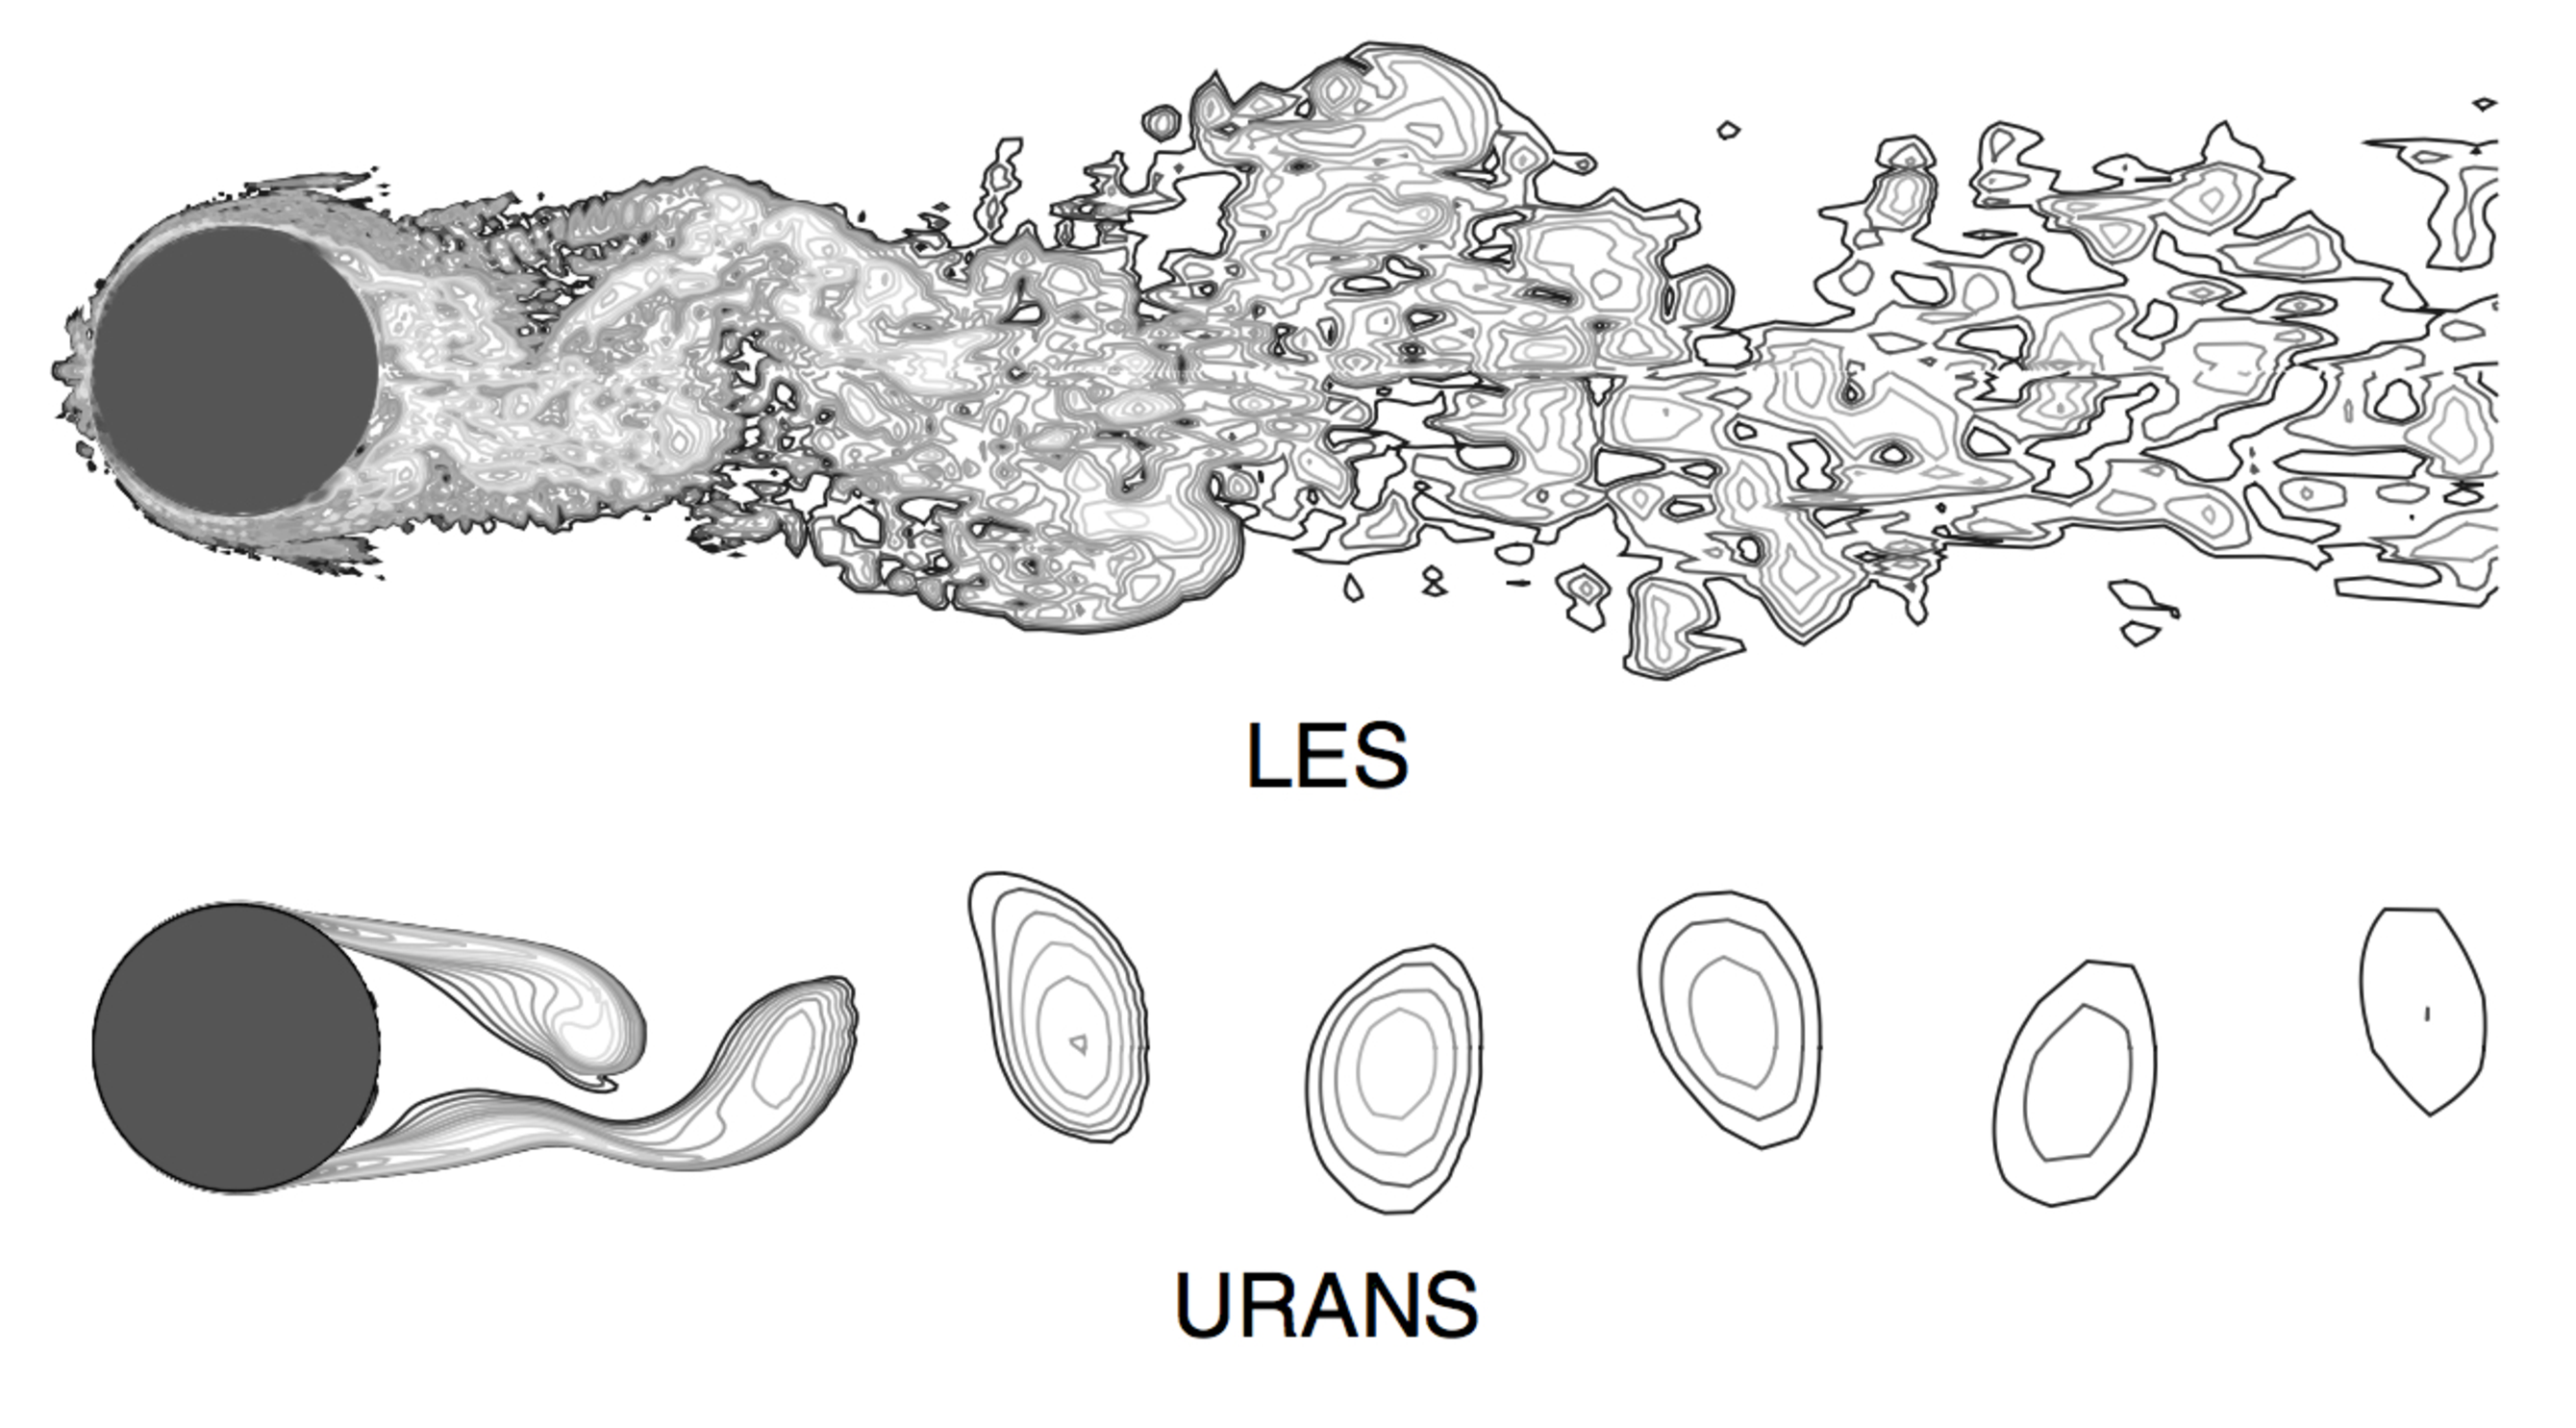
\includegraphics[width=0.45\textwidth]{Images/logan/catalano_2003numerical_UnsteadyURANSvsLES.pdf}
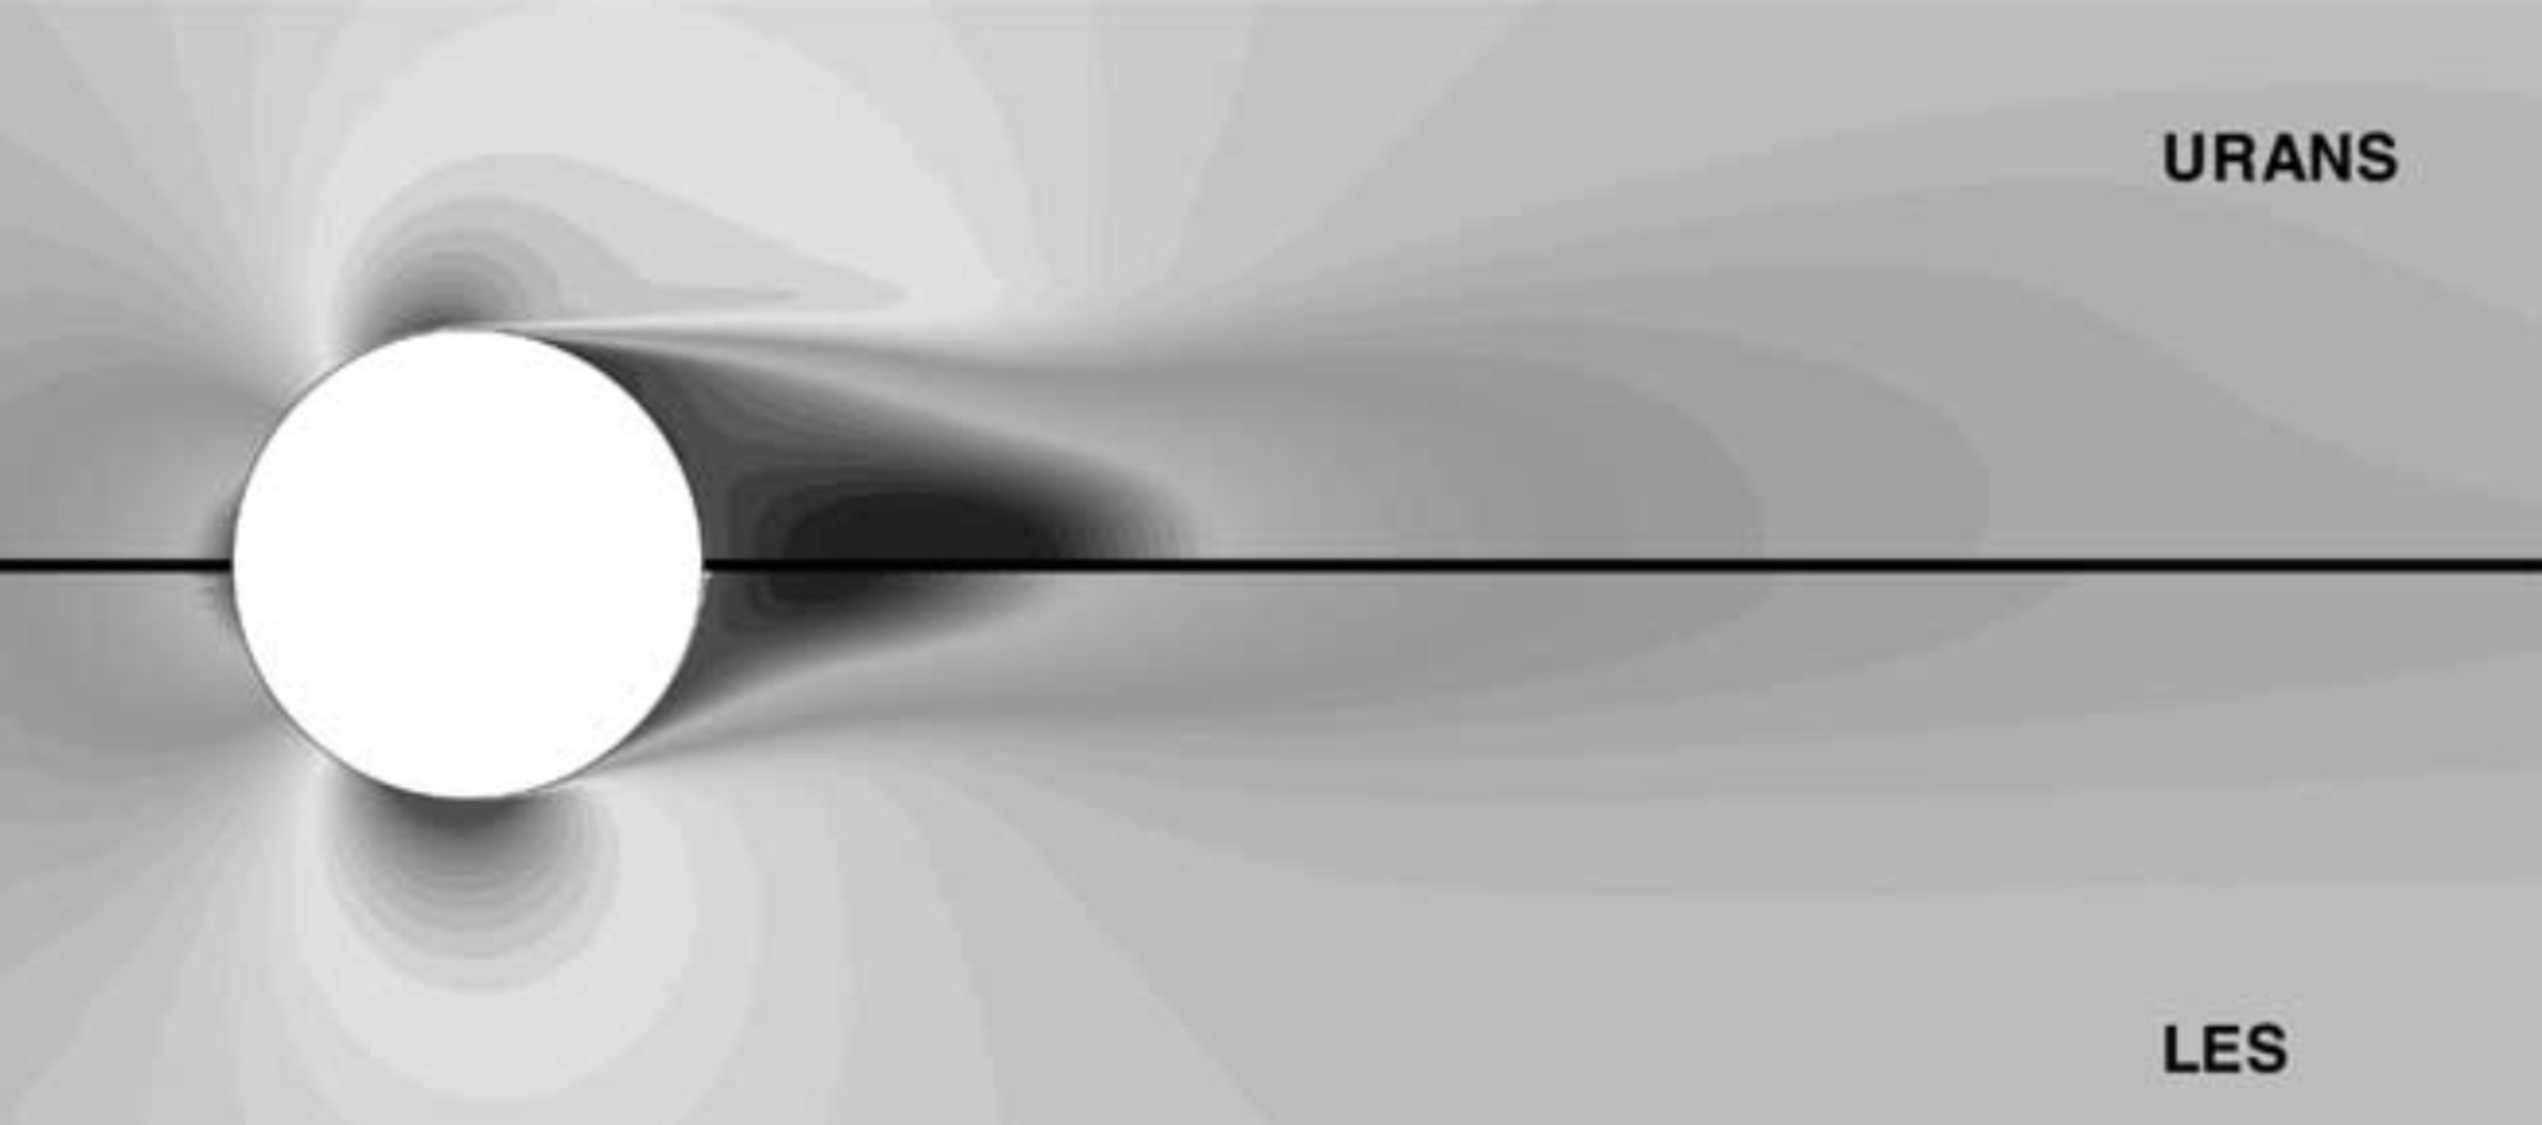
\includegraphics[width=0.54\textwidth]{Images/logan/catalano_2003numerical_SteadyURANSvsLES.pdf}
\caption{ Instantaneous vorticity magnitude (left) and time-averaged streamwise velocity distribution of numeric solutions for circular cylinder at $Re_D = 1.0 \times 10^6$ \cite{catalano2003numerical} }
\label{fig:cylinderransvslesflow}
\end{center}
\end{figure}
%%\vspace{-2em}


Quantitative comparison of the two methodologies against experiment can be found in Fig~\ref{fig:cylinderransvslesvalidation}. To the left, it can be seen that LES matches both the suction peak before separation (near $\theta=90^o$) and the constant base pressure in the separated wake ($\theta=130-180^o$) of the $Re_D = 1.2 \times 10^6$ experiment more closely than URANS.

However, the advantage of LES over URANS in this application diminishes with increasing Reynolds number since more grid refinement is required by LES to resolve finer turbulence scales. Thus, as can be seen in the right of Fig~\ref{fig:cylinderransvslesvalidation}, URANS begins to predict drag coefficient more correctly at higher Reynolds numbers using the same computational resources as the $Re_D = 1.2 \times 10^6$ case.





%%% CYLINDER RANS VS LES VALIDATION
%%\vspace{-2em}
% \begin{figure}[htb]
\begin{figure}[H]
\begin{center}
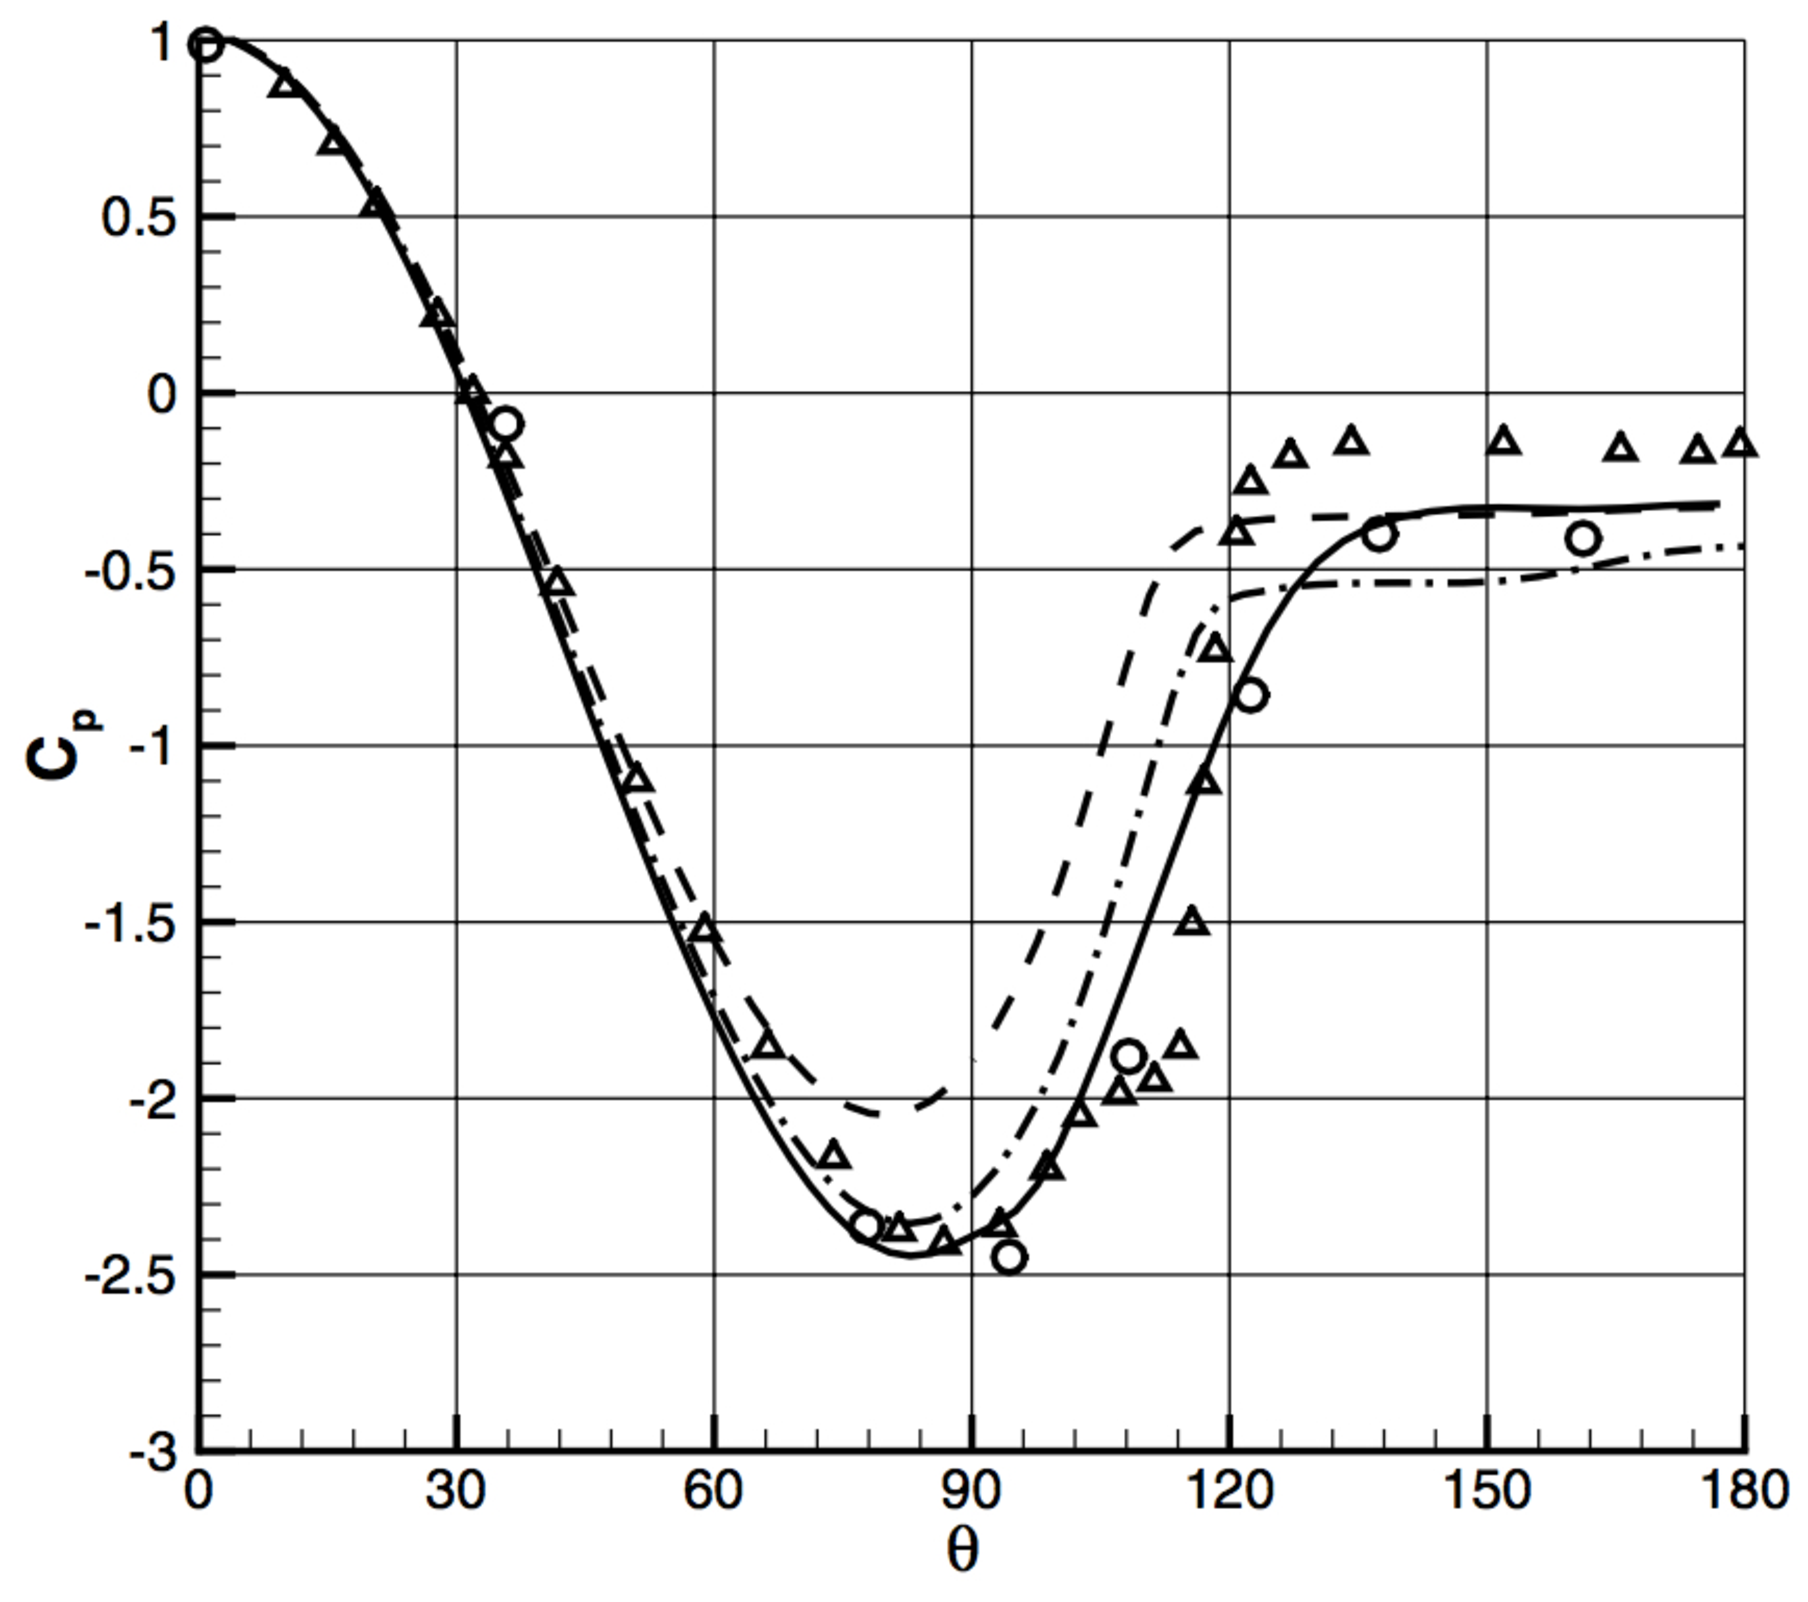
\includegraphics[width=0.49\textwidth]{Images/logan/catalano2003numerical_CylinderCp.pdf}
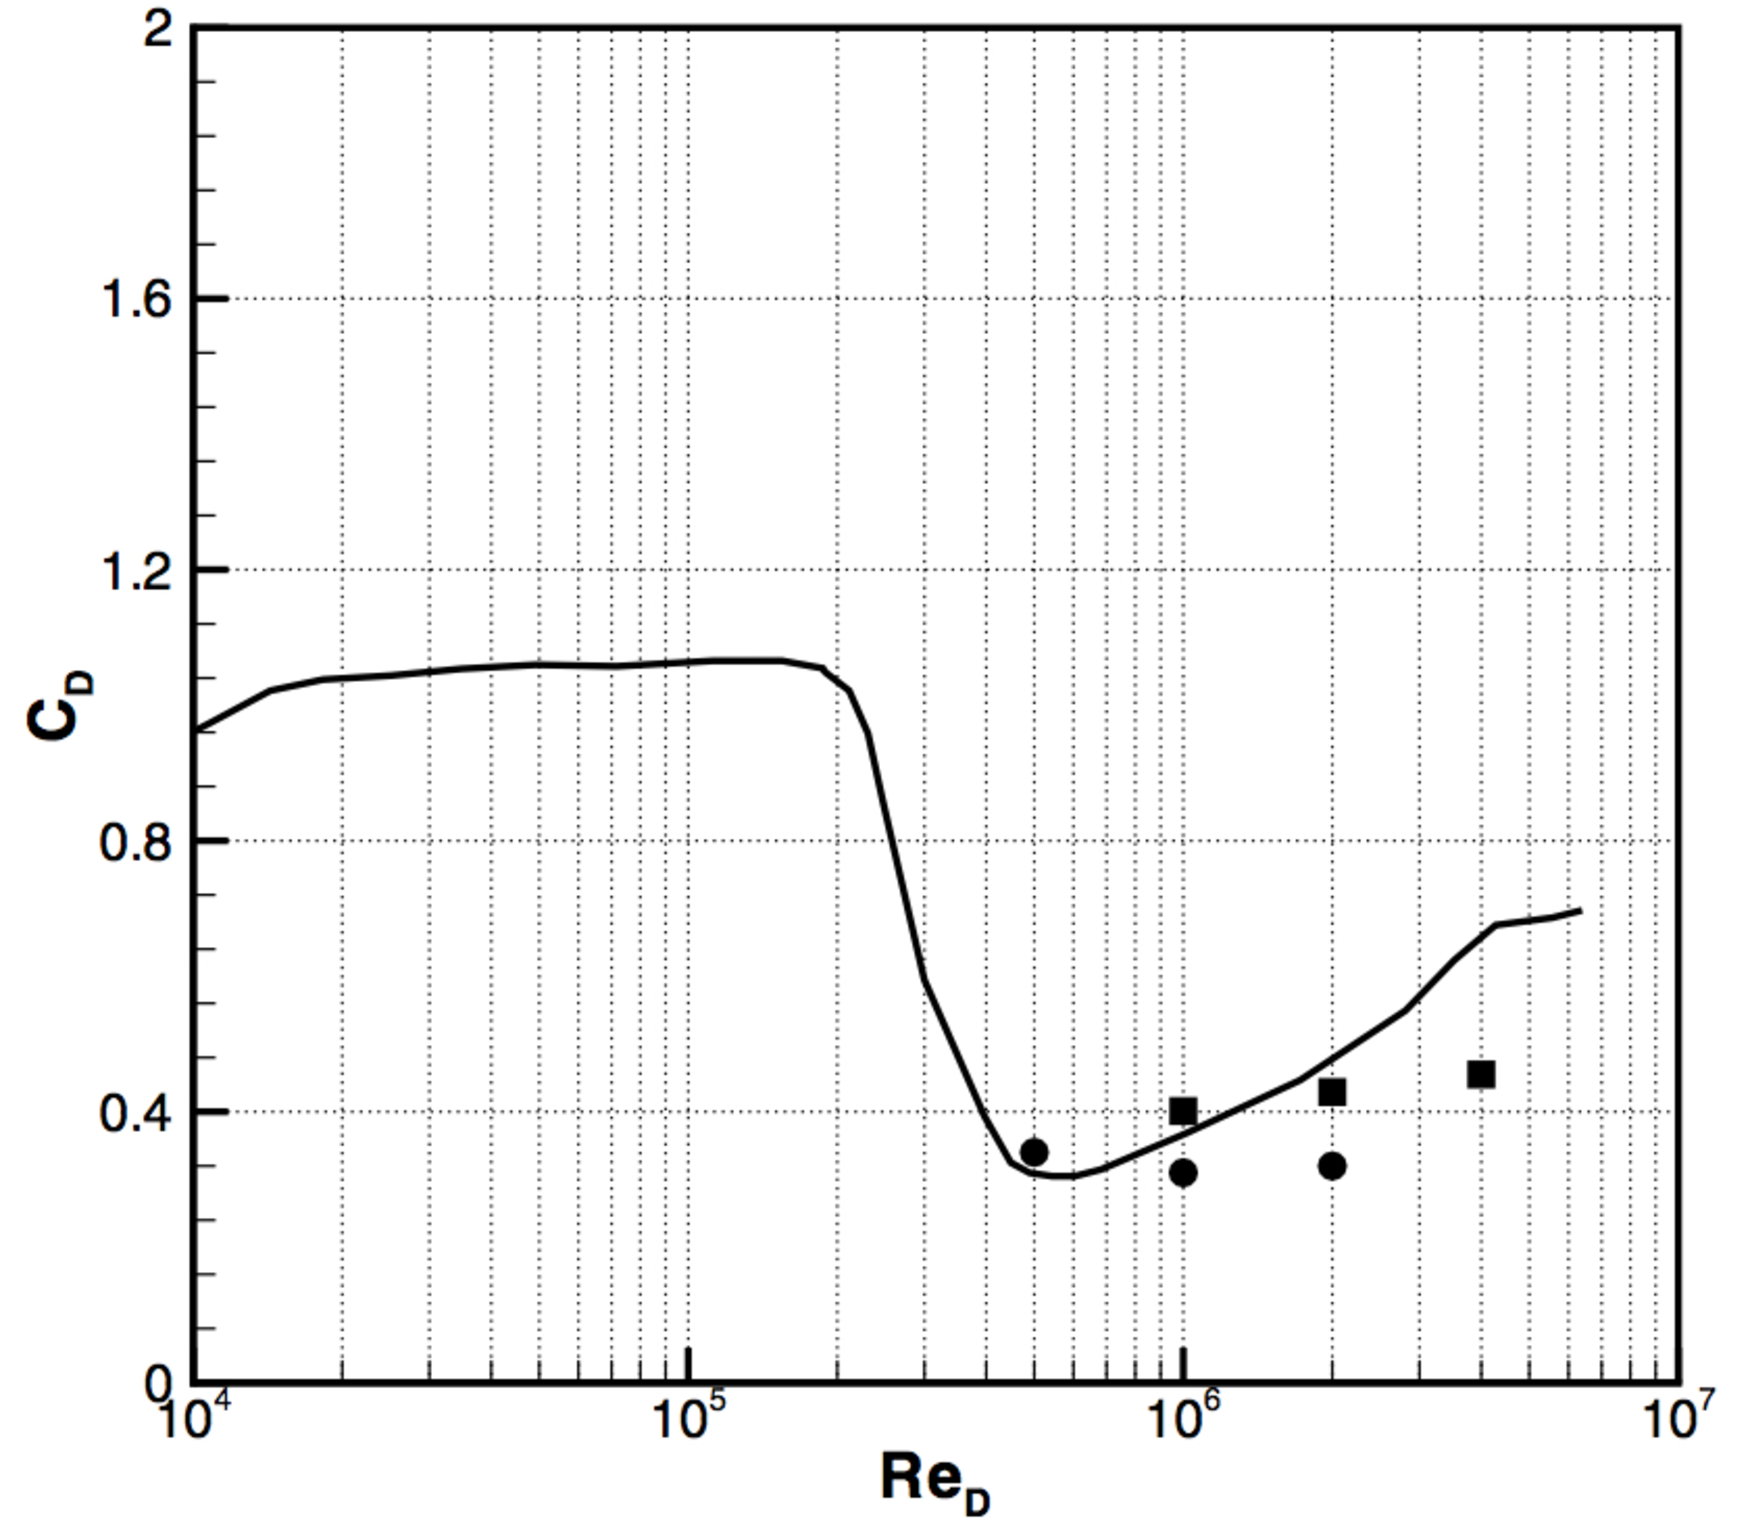
\includegraphics[width=0.49\textwidth]{Images/logan/catalano2003numerical_CylinderDrag.pdf}
\caption{ Mean surface pressure distribution on a cylinder (left) for computational methods: (---) LES, (- -) RANS, (-.-) URANS at $Re_D = 1.0 \times 10^6$ and experiments at (o) $Re_D = 1.2 \times 10^6$ and ($\triangle$) $Re_D = 6.7 \times 10^5$ and computed cylinder drag coefficient as a function of Reynolds number (right) for (--) experiment, (o) LES, and ($\Box$) URANS \cite{catalano2003numerical} }
\label{fig:cylinderransvslesvalidation}
\end{center}
\end{figure}
%%\vspace{-2em}


The results of this study suggest that the undisputed superiority of LES over URANS in resolving instantaneous turbulence of bluff-bodies can remain an advantage in accuracy even when time-averaging is applied. However, this conclusion is case-specific, as URANS can prevail in mean flow prediction accuracy when the flow exceeds the resolution of the LES grid due to the greater computational cost of LES.




















%%% CAPSULE DES VS RANS VS WIND TUNNEL
%%\vspace{-2em}
% \begin{figure}[htb]
\begin{figure}[H]
\begin{center}
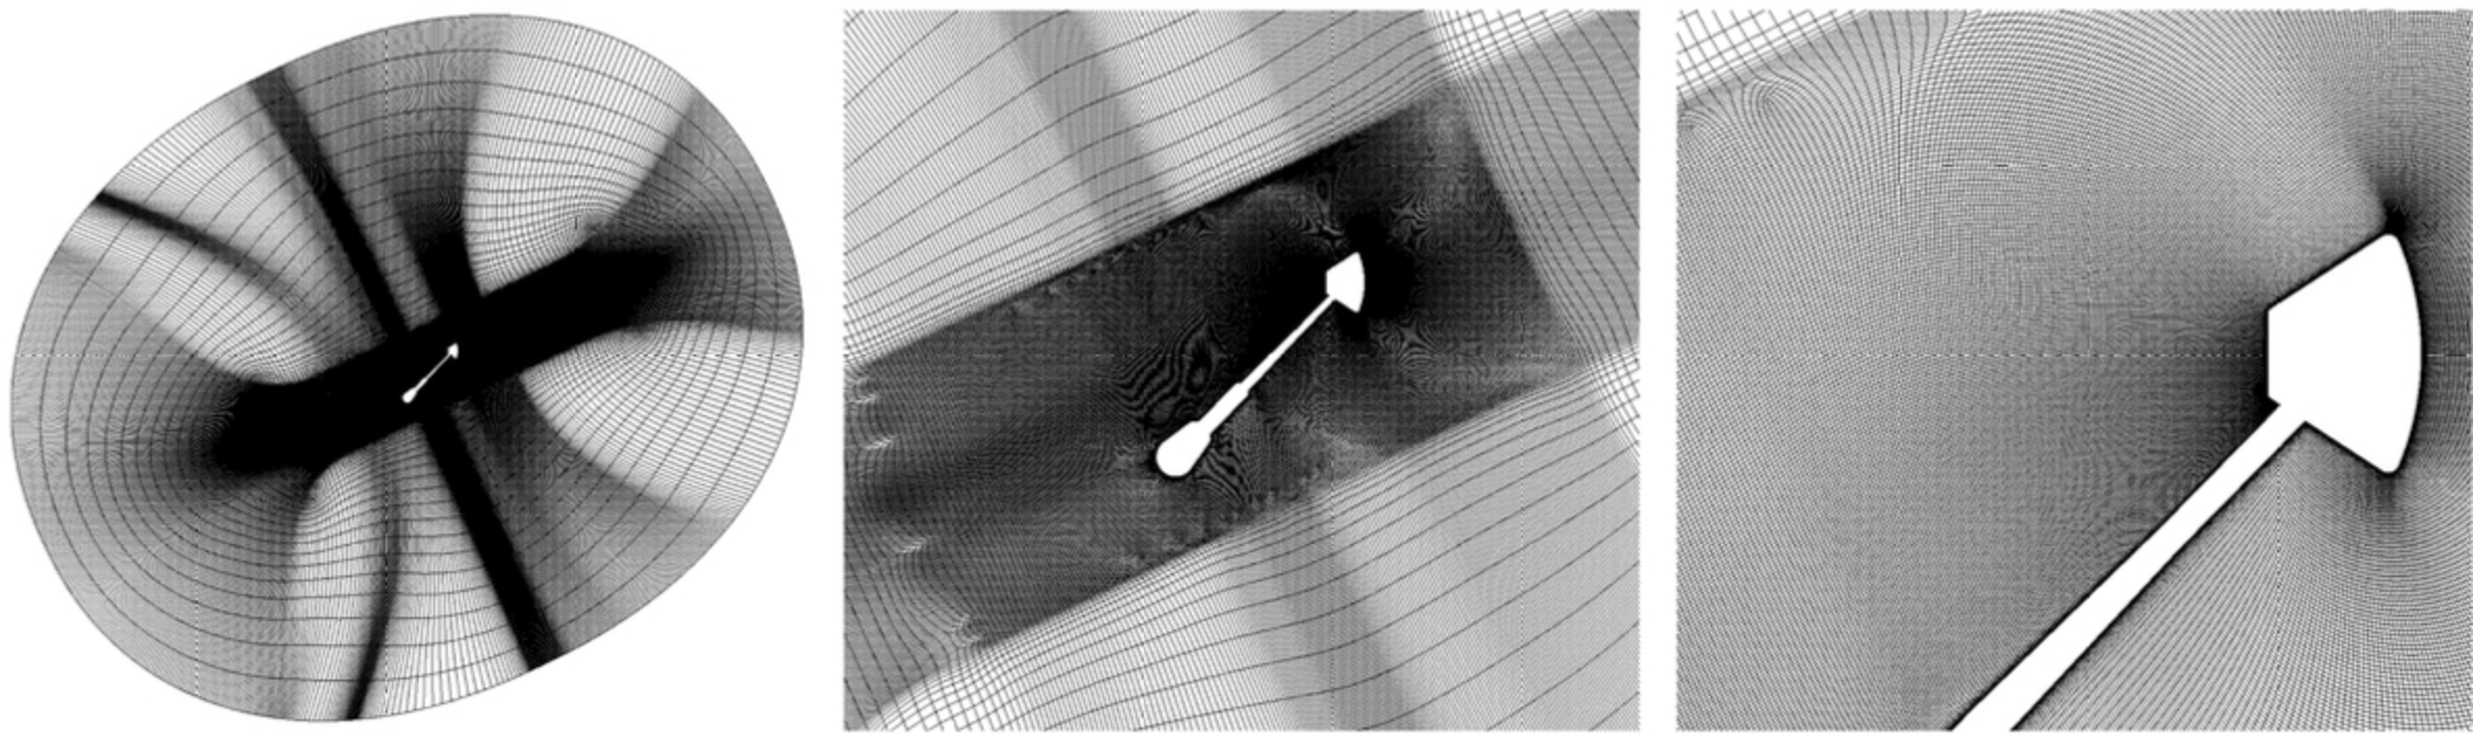
\includegraphics[width=0.95\textwidth]{Images/logan/schwing2015detachededdy_grid.pdf}
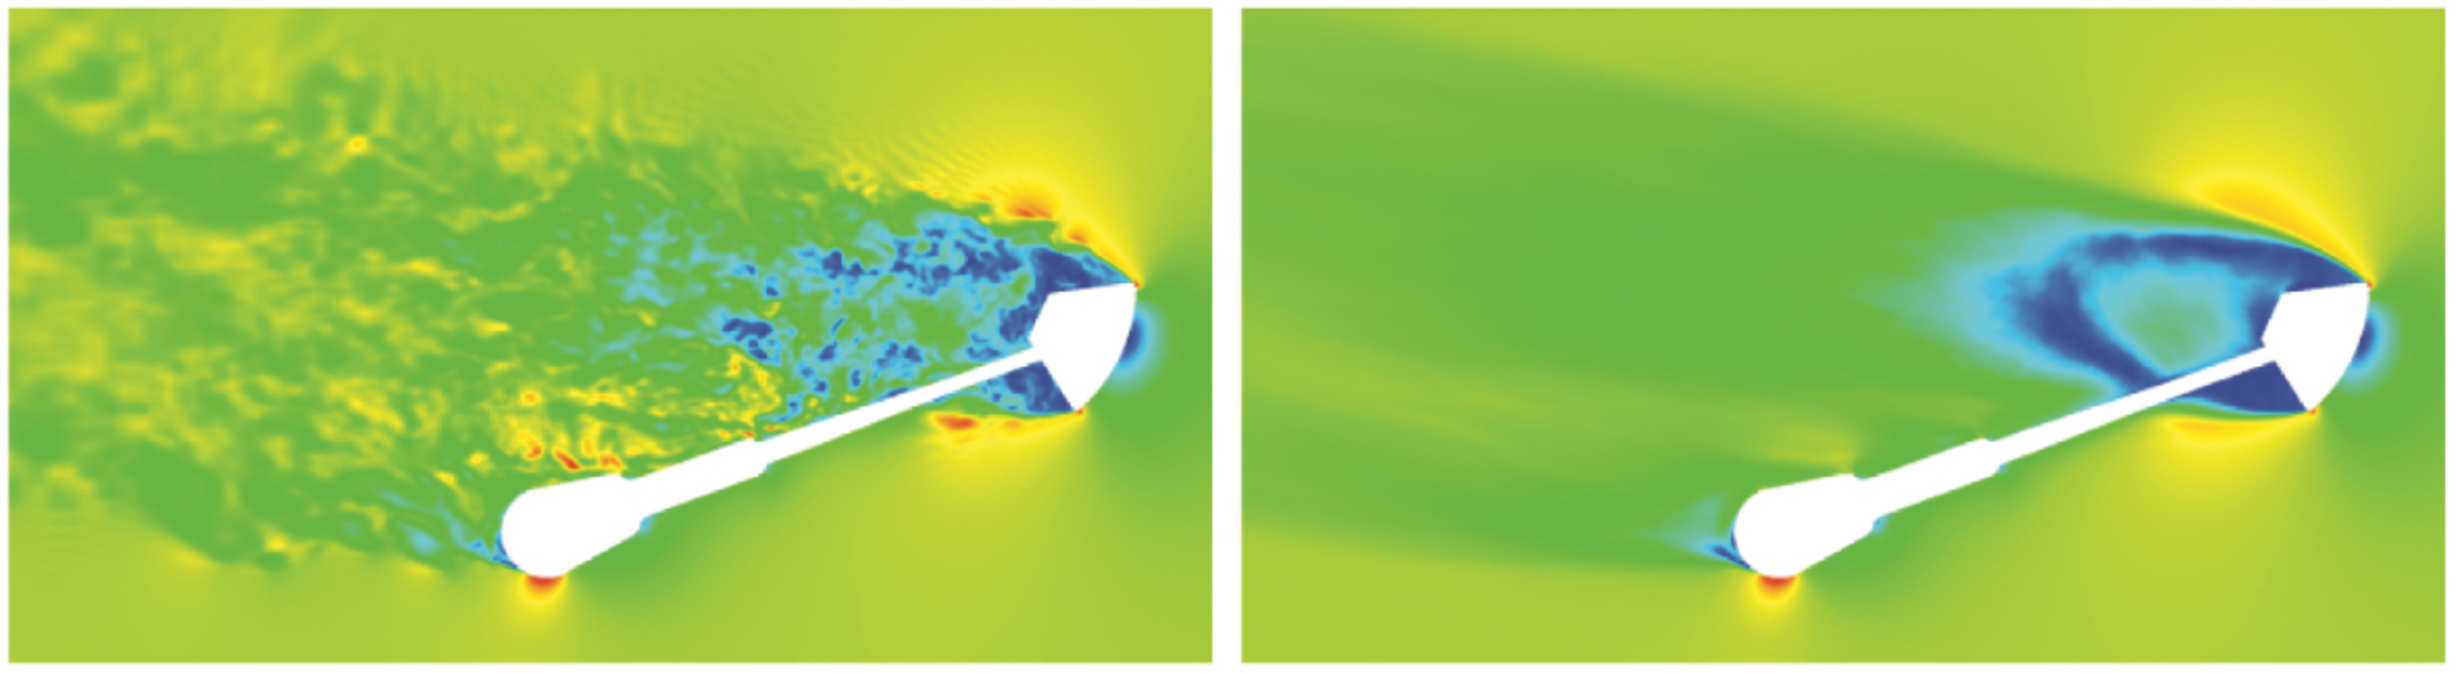
\includegraphics[width=0.95\textwidth]{Images/logan/schwing2015detachededdy_flow.pdf}
\caption{ Orion capsule and wind tunnel sting unstructured grid and instantaneous (left) time-averaged (right) Mach number (DES, $M_{\infty
}=0.5$) \cite{schwing2015detachededdy} }
\label{fig:oriongridflow}
\end{center}
\end{figure}
%%\vspace{-2em}

Next, the functionality of DES (a close sibling to LES with less computational demand) will be compared to URANS for the applied bluff-body case of an atmospheric reentry capsule during the subsonic portion of its trajectory at notably high $Re=5.0 \times 10^6$.  The study by Schwing et al. (2009) \cite{schwing2015detachededdy} compared DES and URANS simulations of the Orion capsule at subsonic and transonic Mach numbers to wind tunnel pressure data. Analysis of the prediction both the instantaneous and mean turbulence features was performed in the study, but this analysis will focus on the accuracy of the simulations with regards to the time-averaged results during subsonic flight.

The mean surface pressure results for each CFD method are presented in the top image of Fig~\ref{fig:orionpressure} for $\alpha=155^o$ and are compared to the mean pressures measured by the taps in the wind tunnel test. In this example, it is obvious that the DES-KES method (which will be referred to as DES for the remainder of this section) predicts the backshell pressure distribution with vastly superior accuracy to its URANS equivalent. This advantage does not occur in all tested conditions, however, as there are many cases where the less-expensive URANS formulation produces compatible pressure distributions to DES.

A more quantitative analysis capsule wake prediction accuracy of each model is supplied in the lower image of Fig~\ref{fig:orionpressure}, which is a line plot of the surface pressure in taps along the centerline of the capsule's cross-section. Here, two suction peaks can be seen near X/D=0.75, which correspond to the flow separation at the capsule shoulder that can be seen in Fig~\ref{fig:oriongridflow}. The magnitude of each of these peaks is most closely predicted by DES. In addition, the nearly constant base pressure on the backshell of the capsule in the separated wake is very accurately predicted by DES, while the URANS equivalent is incorrect in both magnitude and in its varying nature.  These differences in wake behavior prediction result in a much more accurate drag prediction by DES in comparison to wind tunnel results. However, DES was not the overall victor in mean load prediction since the integration of lift of for the URANS pressure distribution proved to be more accurate. The author attributes this discrepancy to separation prediction, which highlights the potential ambiguity of hybrid RANS/LES behavior in response to grid and geometry.






%CAPSULE SURFACE PRESSURE
%%\vspace{-2em}
% \begin{figure}[htb]
\begin{figure}[H]
\begin{center}
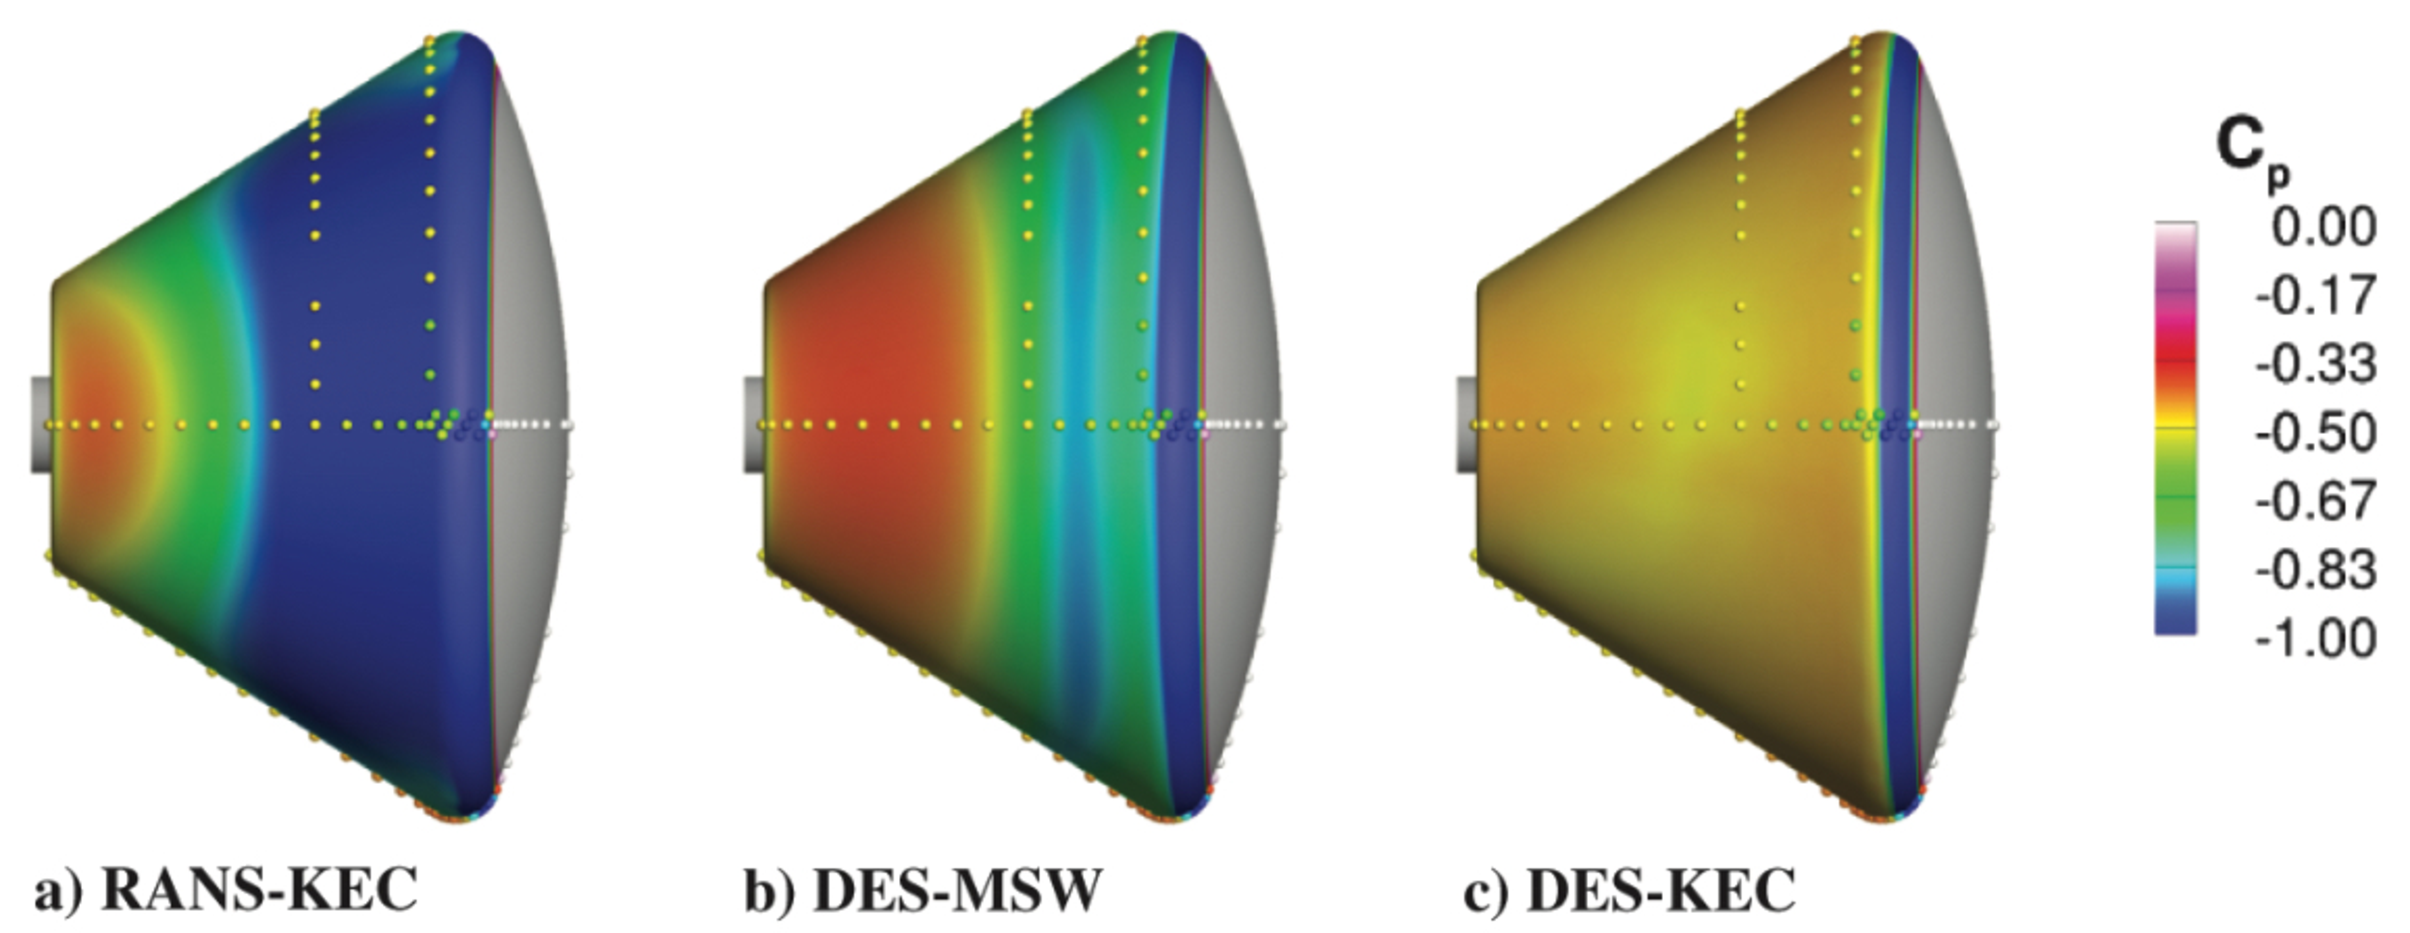
\includegraphics[width=0.95\textwidth]{Images/logan/schwing2015detachededdy_surfacepressure.pdf}
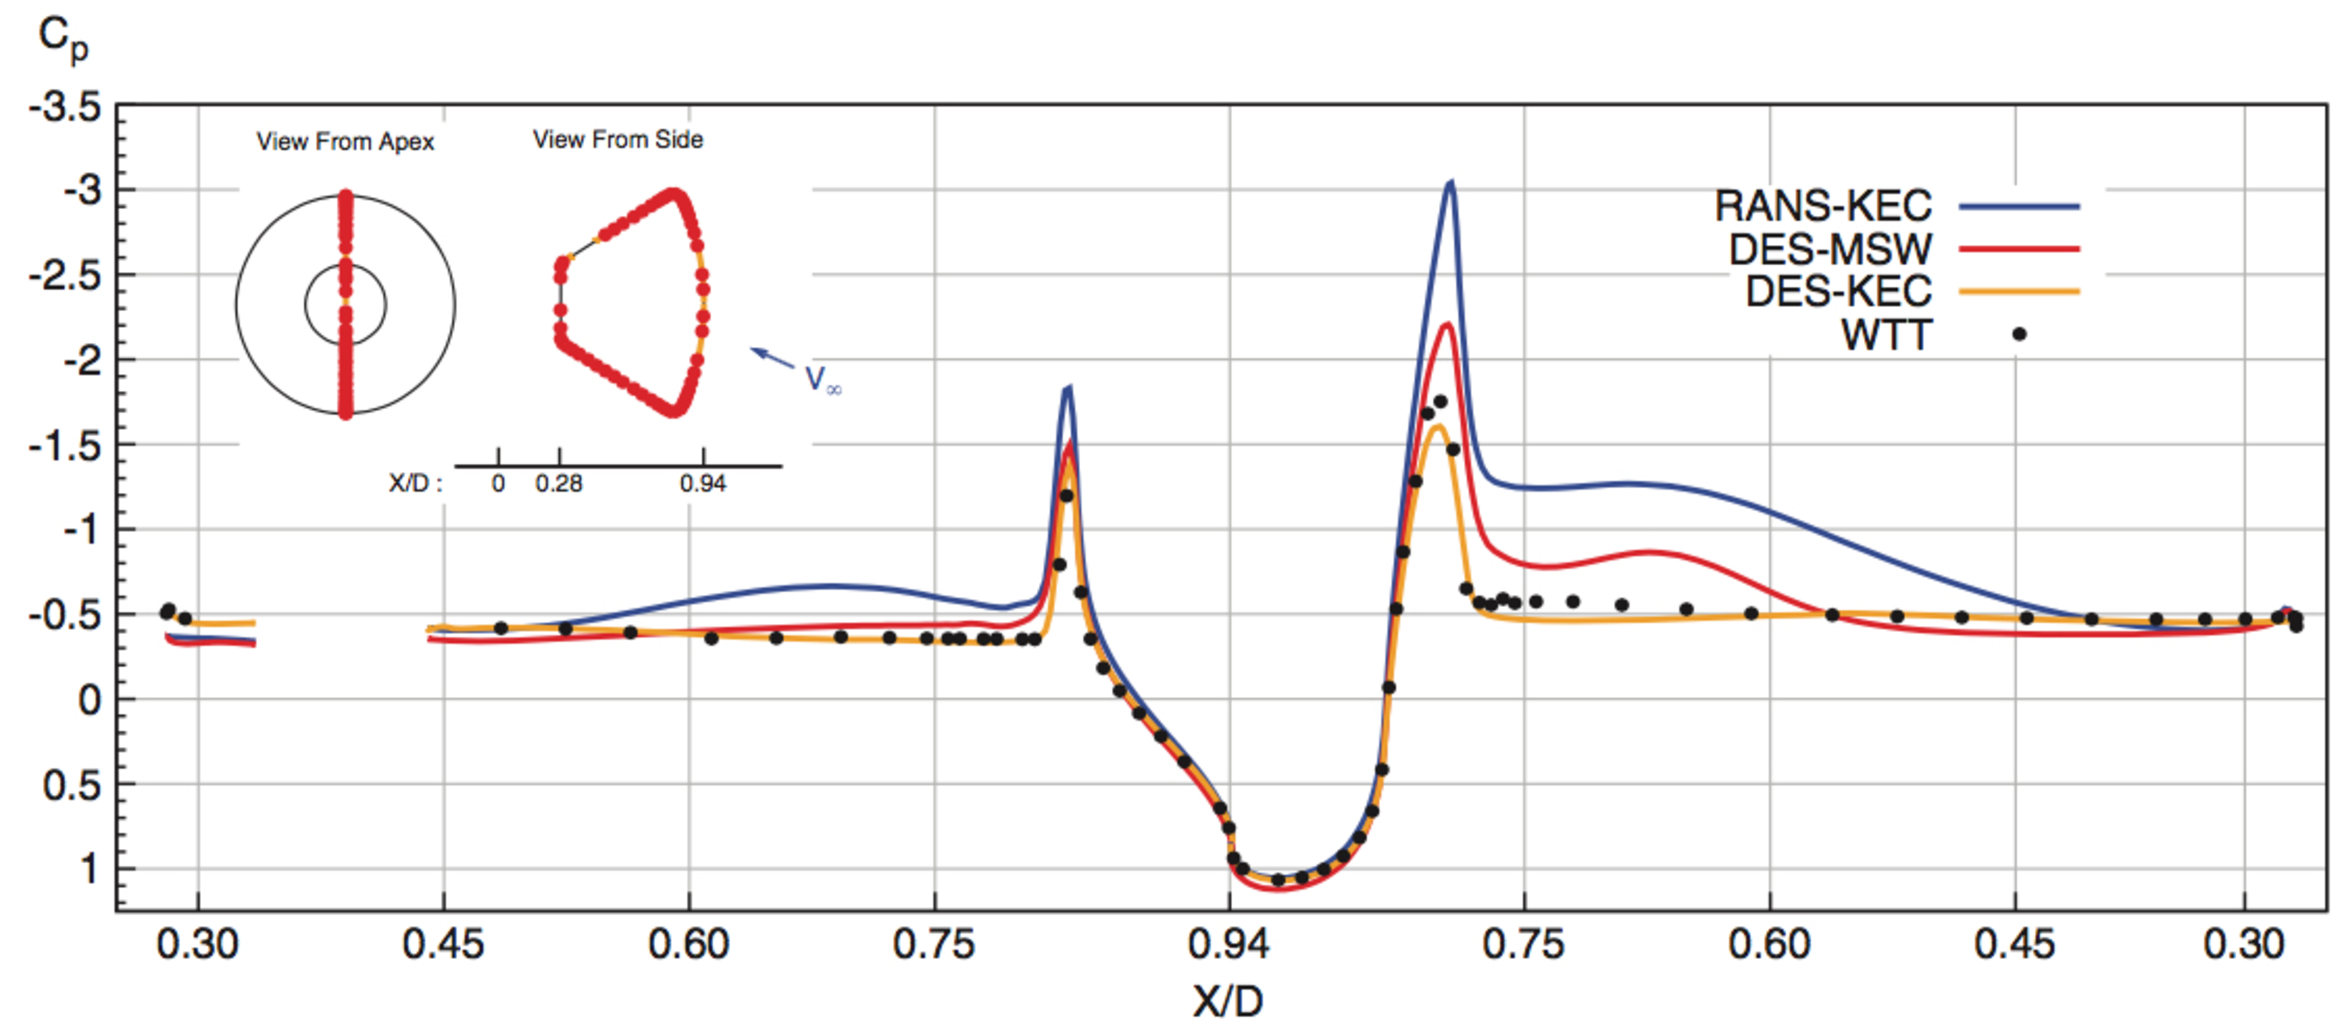
\includegraphics[width=0.95\textwidth]{Images/logan/schwing2015detachededdy_surfacetaps.pdf}
\caption{ Top: Mean simulation surface pressure contours compared to wind tunnel test (WTT) freckle plot. Bottom: Line plots of pressure tap data along a surface cross-section ($M_{\infty}=0.5,\;\alpha=155^o$) \cite{schwing2015detachededdy} }
\label{fig:orionpressure}
\end{center}
\end{figure}
%%\vspace{-2em}


The results of this study demonstrate that CFD techniques are mature enough to accurately simulate complex, realistic bluff-body flows like this high-Reynolds number reentry capsule.  Both URANS and DES proved capable in many sets of conditions, but the increased computational cost of DES became more justified at high angle of attack flight conditions where URANS was insufficient for accurate wake modeling.  The ambiguity of mean load prediction accuracy between methods demonstrates that no one method is superior for all conditions and that user intuition toward flow realism is still an essential component of an accurate bluff-body simulation.





%%%%%%%%%%%%%%%%%%%%%%%%%%%%%%%%%%%%%%%%%%%%%%%%%%%%%%%%%%%%%%%%%%%%%%%%
\subsection{Comparison of DES and SAS Methodologies for Bluff-Bodies} \label{subsec:desvssas}






%%% CYLINDER DES VS SAS VALIDATION
%%\vspace{-2em}
% \begin{figure}[htb]
\begin{figure}[H]
\begin{center}
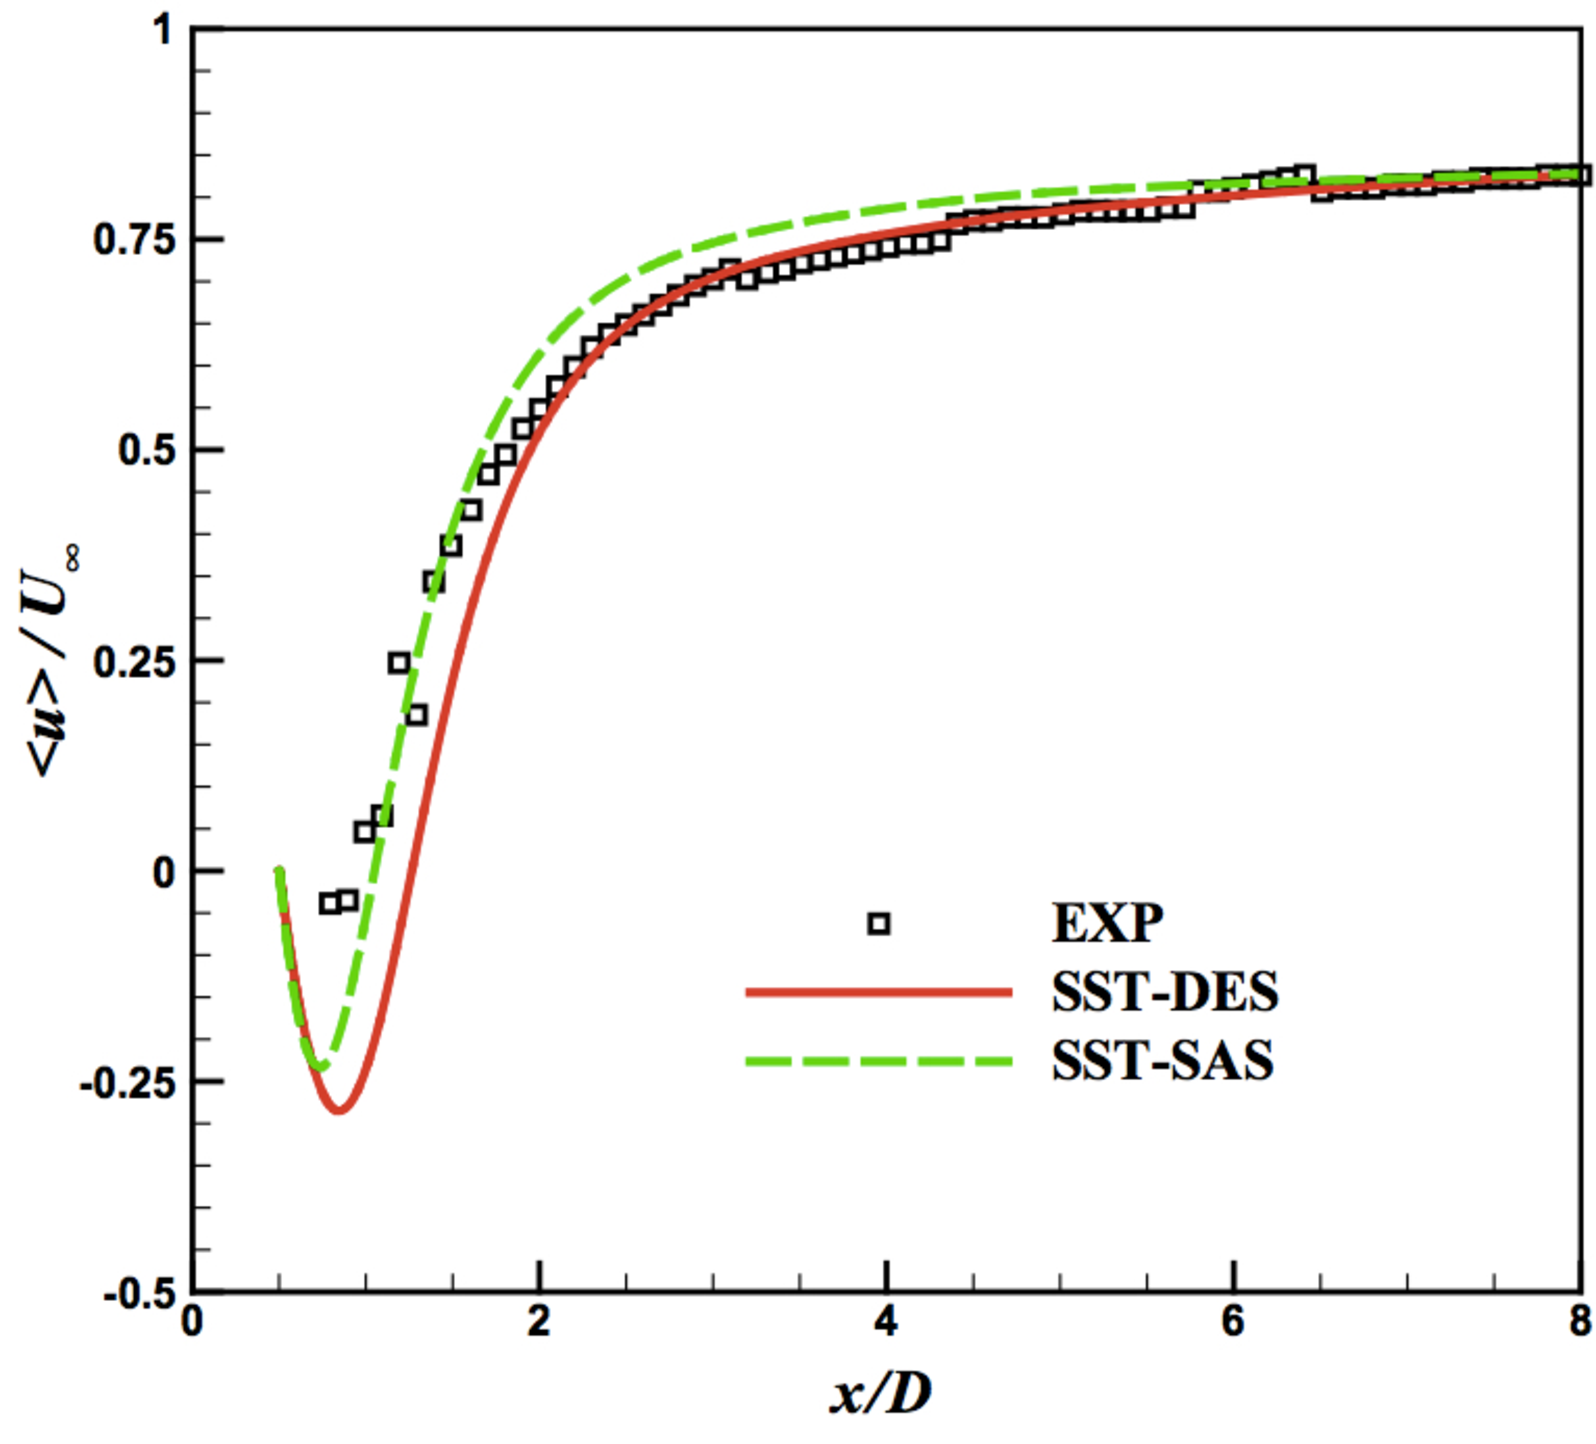
\includegraphics[width=0.49\textwidth]{Images/logan/zheng2016comparative_WakeVelocity.pdf}
% 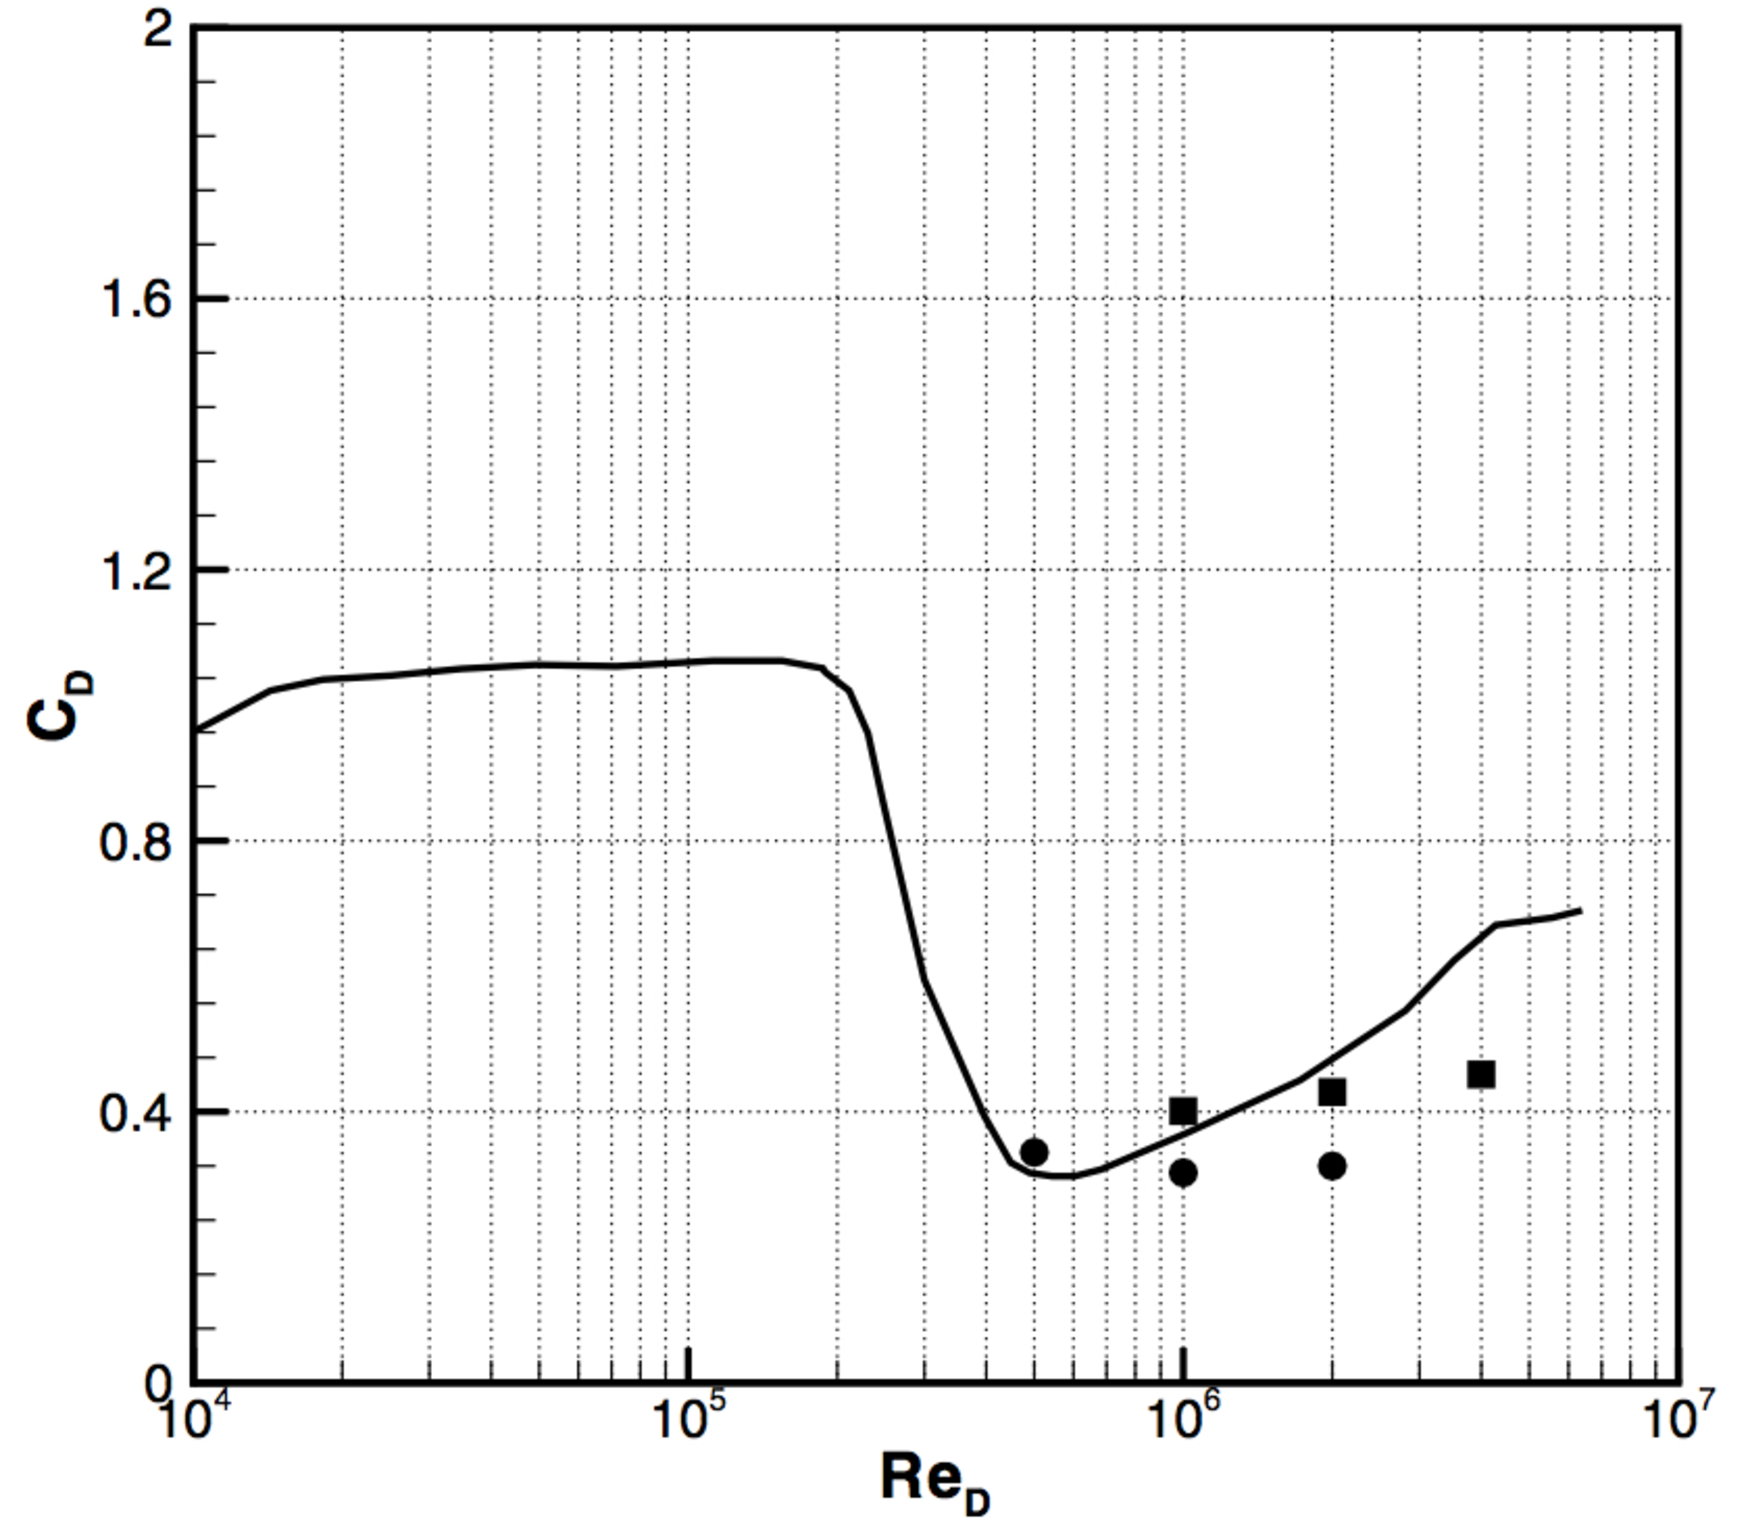
\includegraphics[width=0.49\textwidth]{Images/logan/catalano2003numerical_CylinderDrag.pdf}
\caption{ cylinder des vs sas time-averaged wake velocity \cite{zheng2016comparative} }
\label{fig:cylinderdesvssas}
\end{center}
\end{figure}
%%\vspace{-2em}

$Re_D = 1.4 \times 10^5$, same grid for both solvers, SAS shows good agreement in mean flow properties of near wake, convergence of both solvers in far wake. SAS can have some advantages at same computational cost, SAS is more dissipative,



Preliminary study, Slipstream analysis of high-speed train, DDES was most like experiment but SAS was comparable. Independent grid and time step refinement.

computational cost:
URANS:SAS:DDES = 1:10:20
\cite{wang2017performance}















%%%%%%%%%%%%%%%%%%%%%%%%%%%%%%%%%%%%%%%%%%%%%%%%%%%%%%%%%%%%%%%%%%%%%%%%
\subsection{Complex Bluff-Body Flows with DES} \label{subsec:complexdes}


%%% DES SPHERE DEMONSTRATING COMPARISON TO EXPERIMENT
%%\vspace{-2em}
% \begin{figure}[htb]
\begin{figure}[H]
\begin{center}
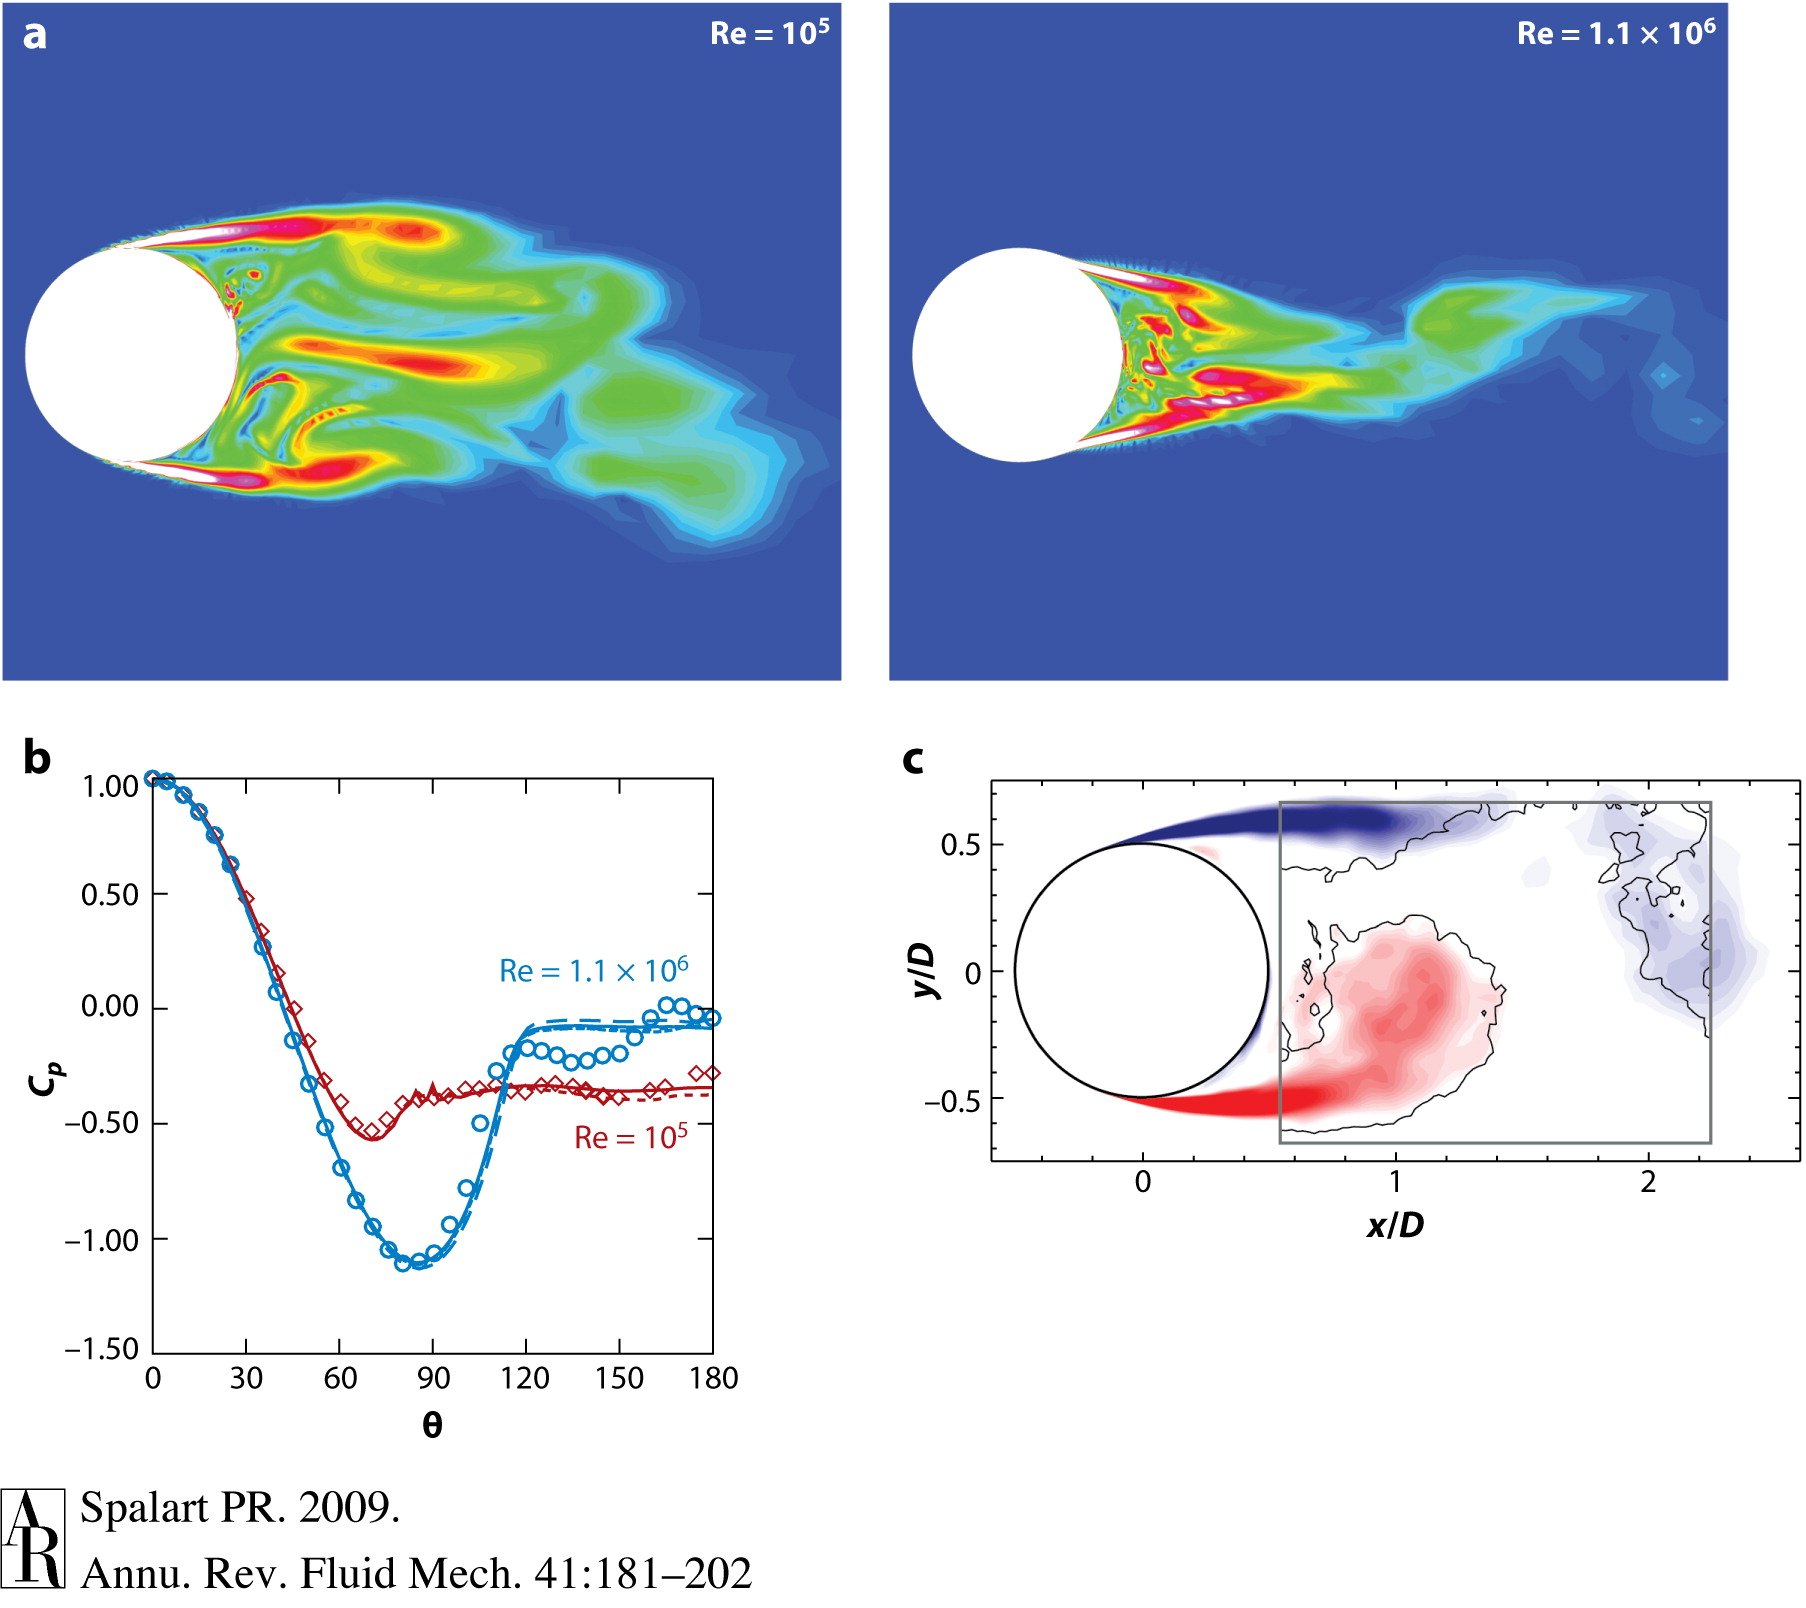
\includegraphics[width=0.8\textwidth]{Images/logan/spalart2009detachededdy_SphereSeparation.jpeg}
\caption{ DES validation from \cite{spalart2009detachededdy}. Sphere transition and drag crisis from \cite{squires2004detachededdy}.  Vorticity validation from \cite{mockett2008demonstration} }
\label{fig:desspherevalidation}
\end{center}
\end{figure}
%%\vspace{-2em}

Simple bluff bodies. (a) Flow visualizations and (b) pressure distributions for a sphere. Re = 105 and 1.1 × 106. Open circles and
diamonds denote experiments, whereas the dotted and dashed lines denote detached-eddy simulation (DES) on two grids. Panels a and
b courtesy of K. Squires. (c) Phase-averaged vorticity contours for a cylinder. Color gradations denote DES conducted by Mockett et al.
(2008), and the solid line denotes experiments by the same authors.

NOTE: DES could be used to emulate the dimples on a golf ball by setting the boundary layer separation point, but true simulation of flow in golf ball dimples requires DNS due to the range of scales










%%% F15 DES
%%\vspace{-2em}
% \begin{figure}[htb]
\begin{figure}[H]
\begin{center}
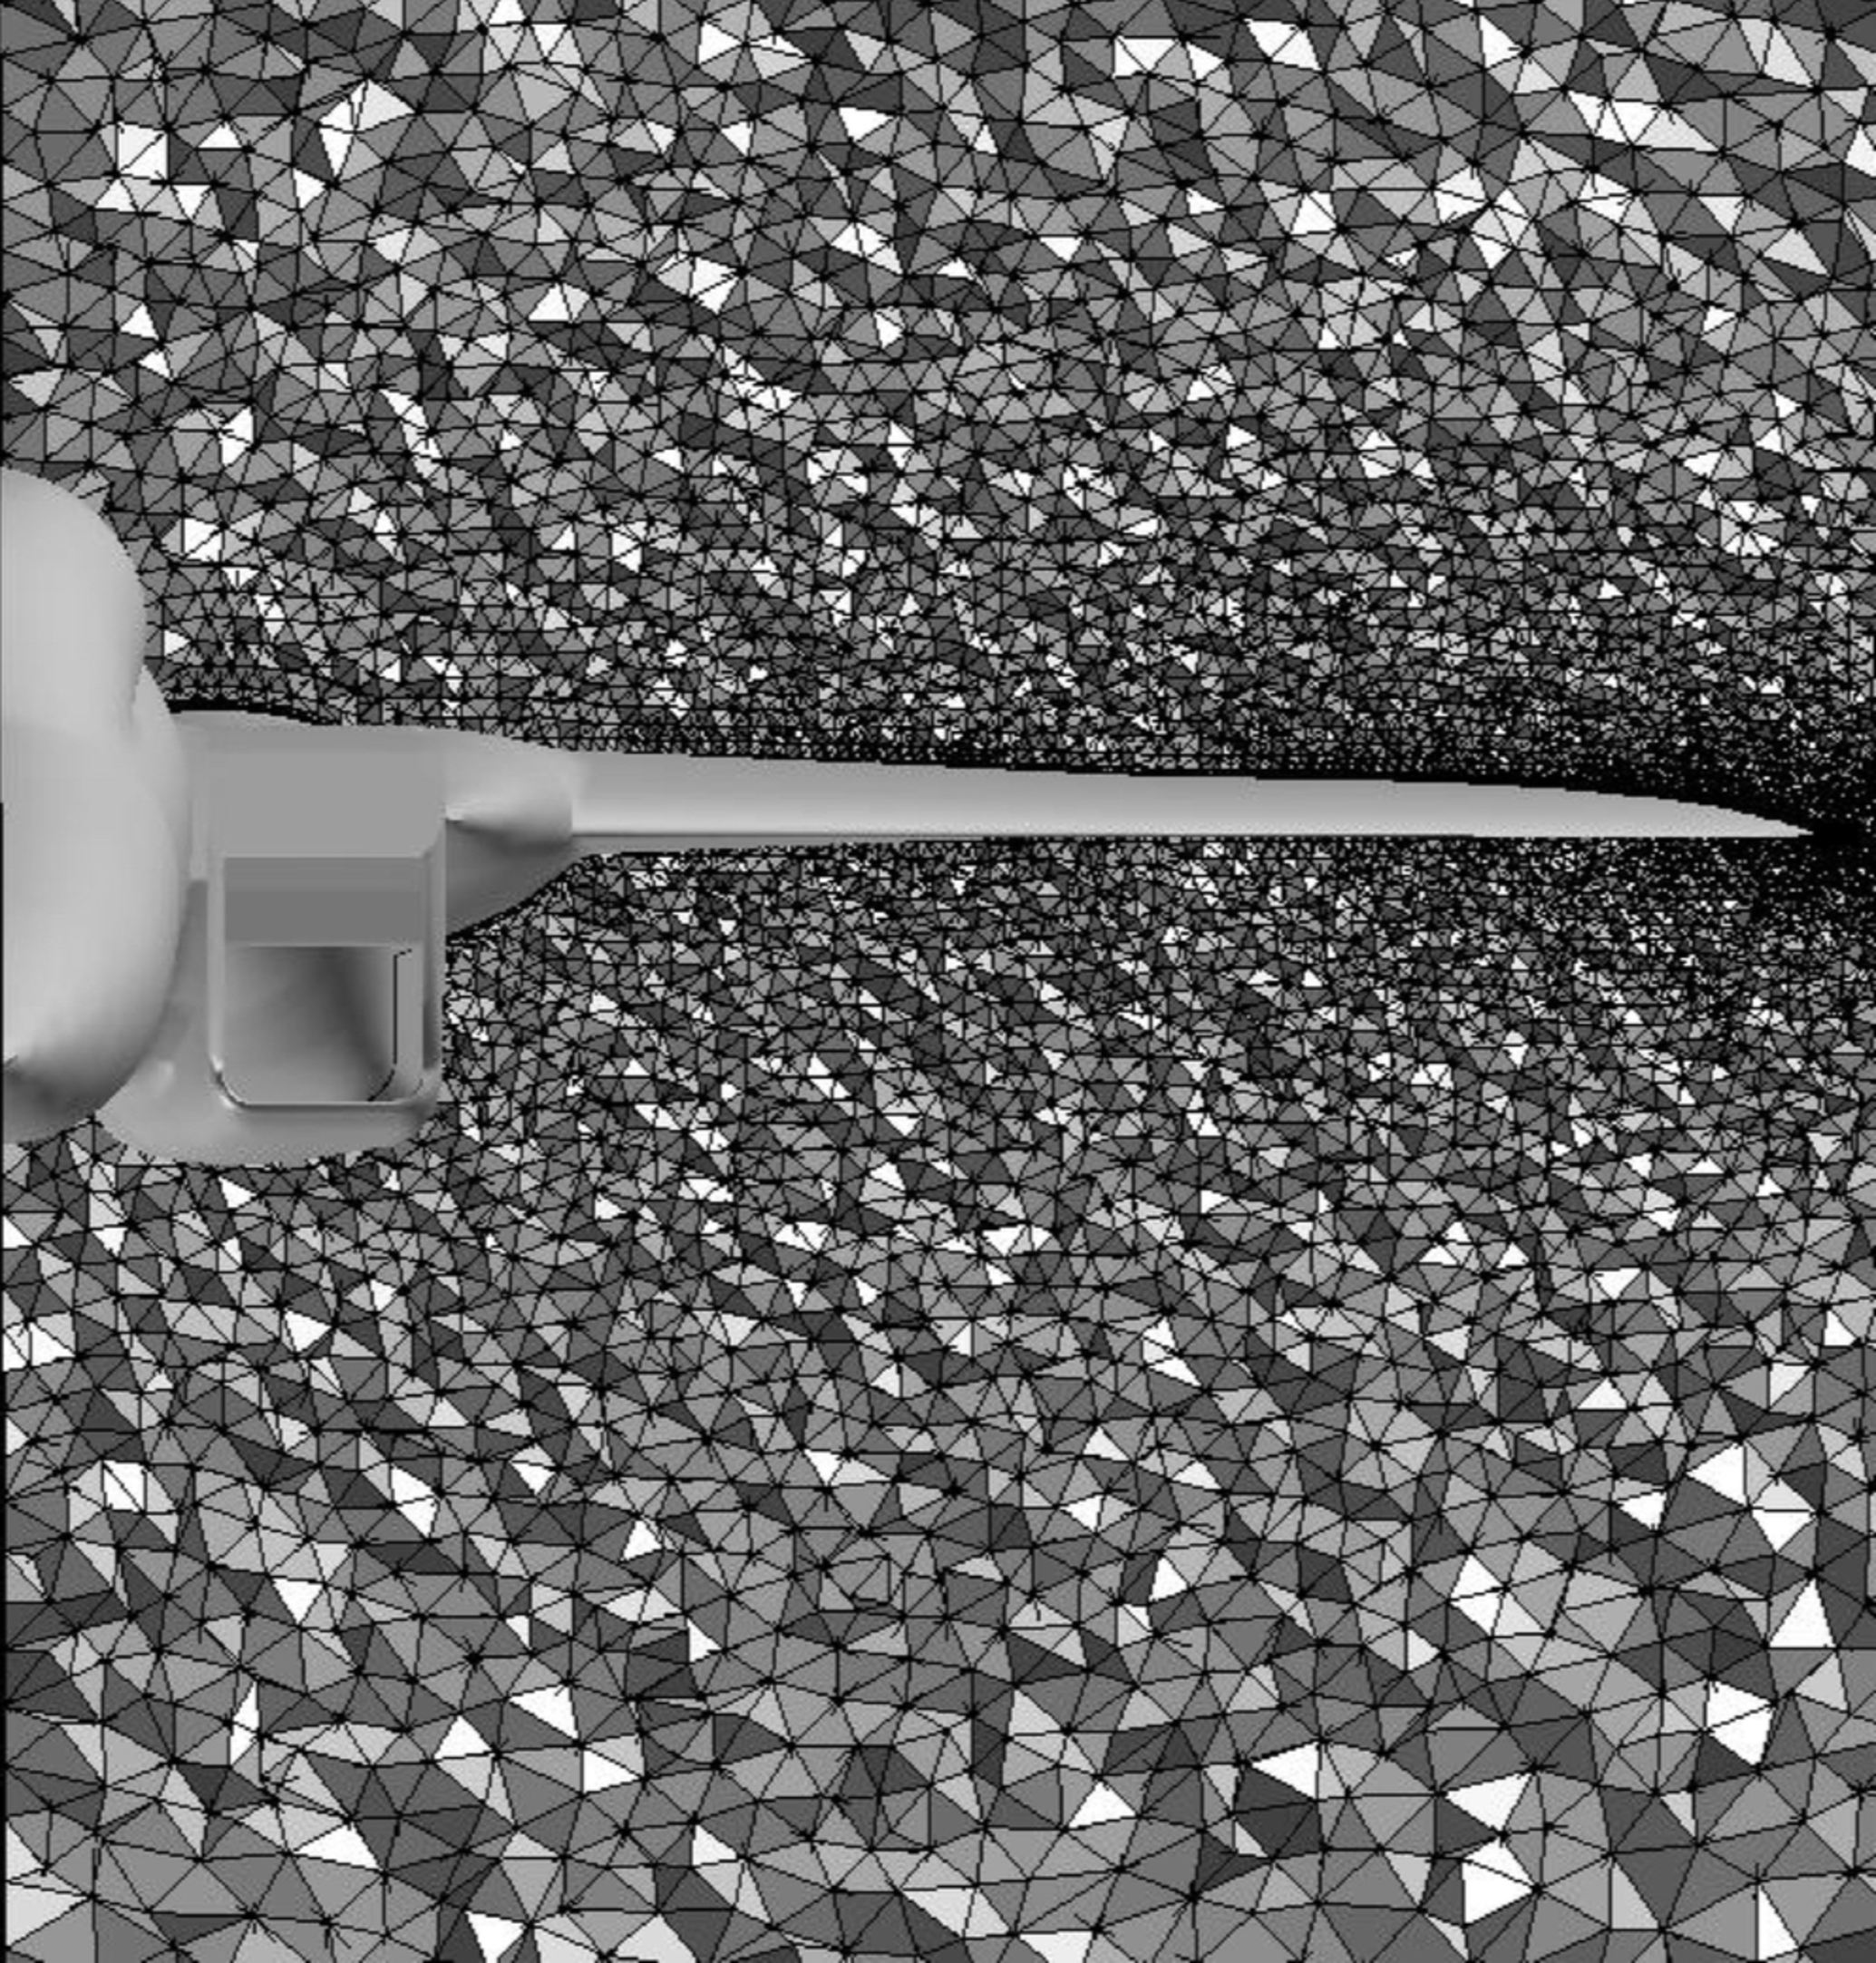
\includegraphics[width=0.45\textwidth]{Images/logan/forsythe2004detachededdy_f15grid.pdf}
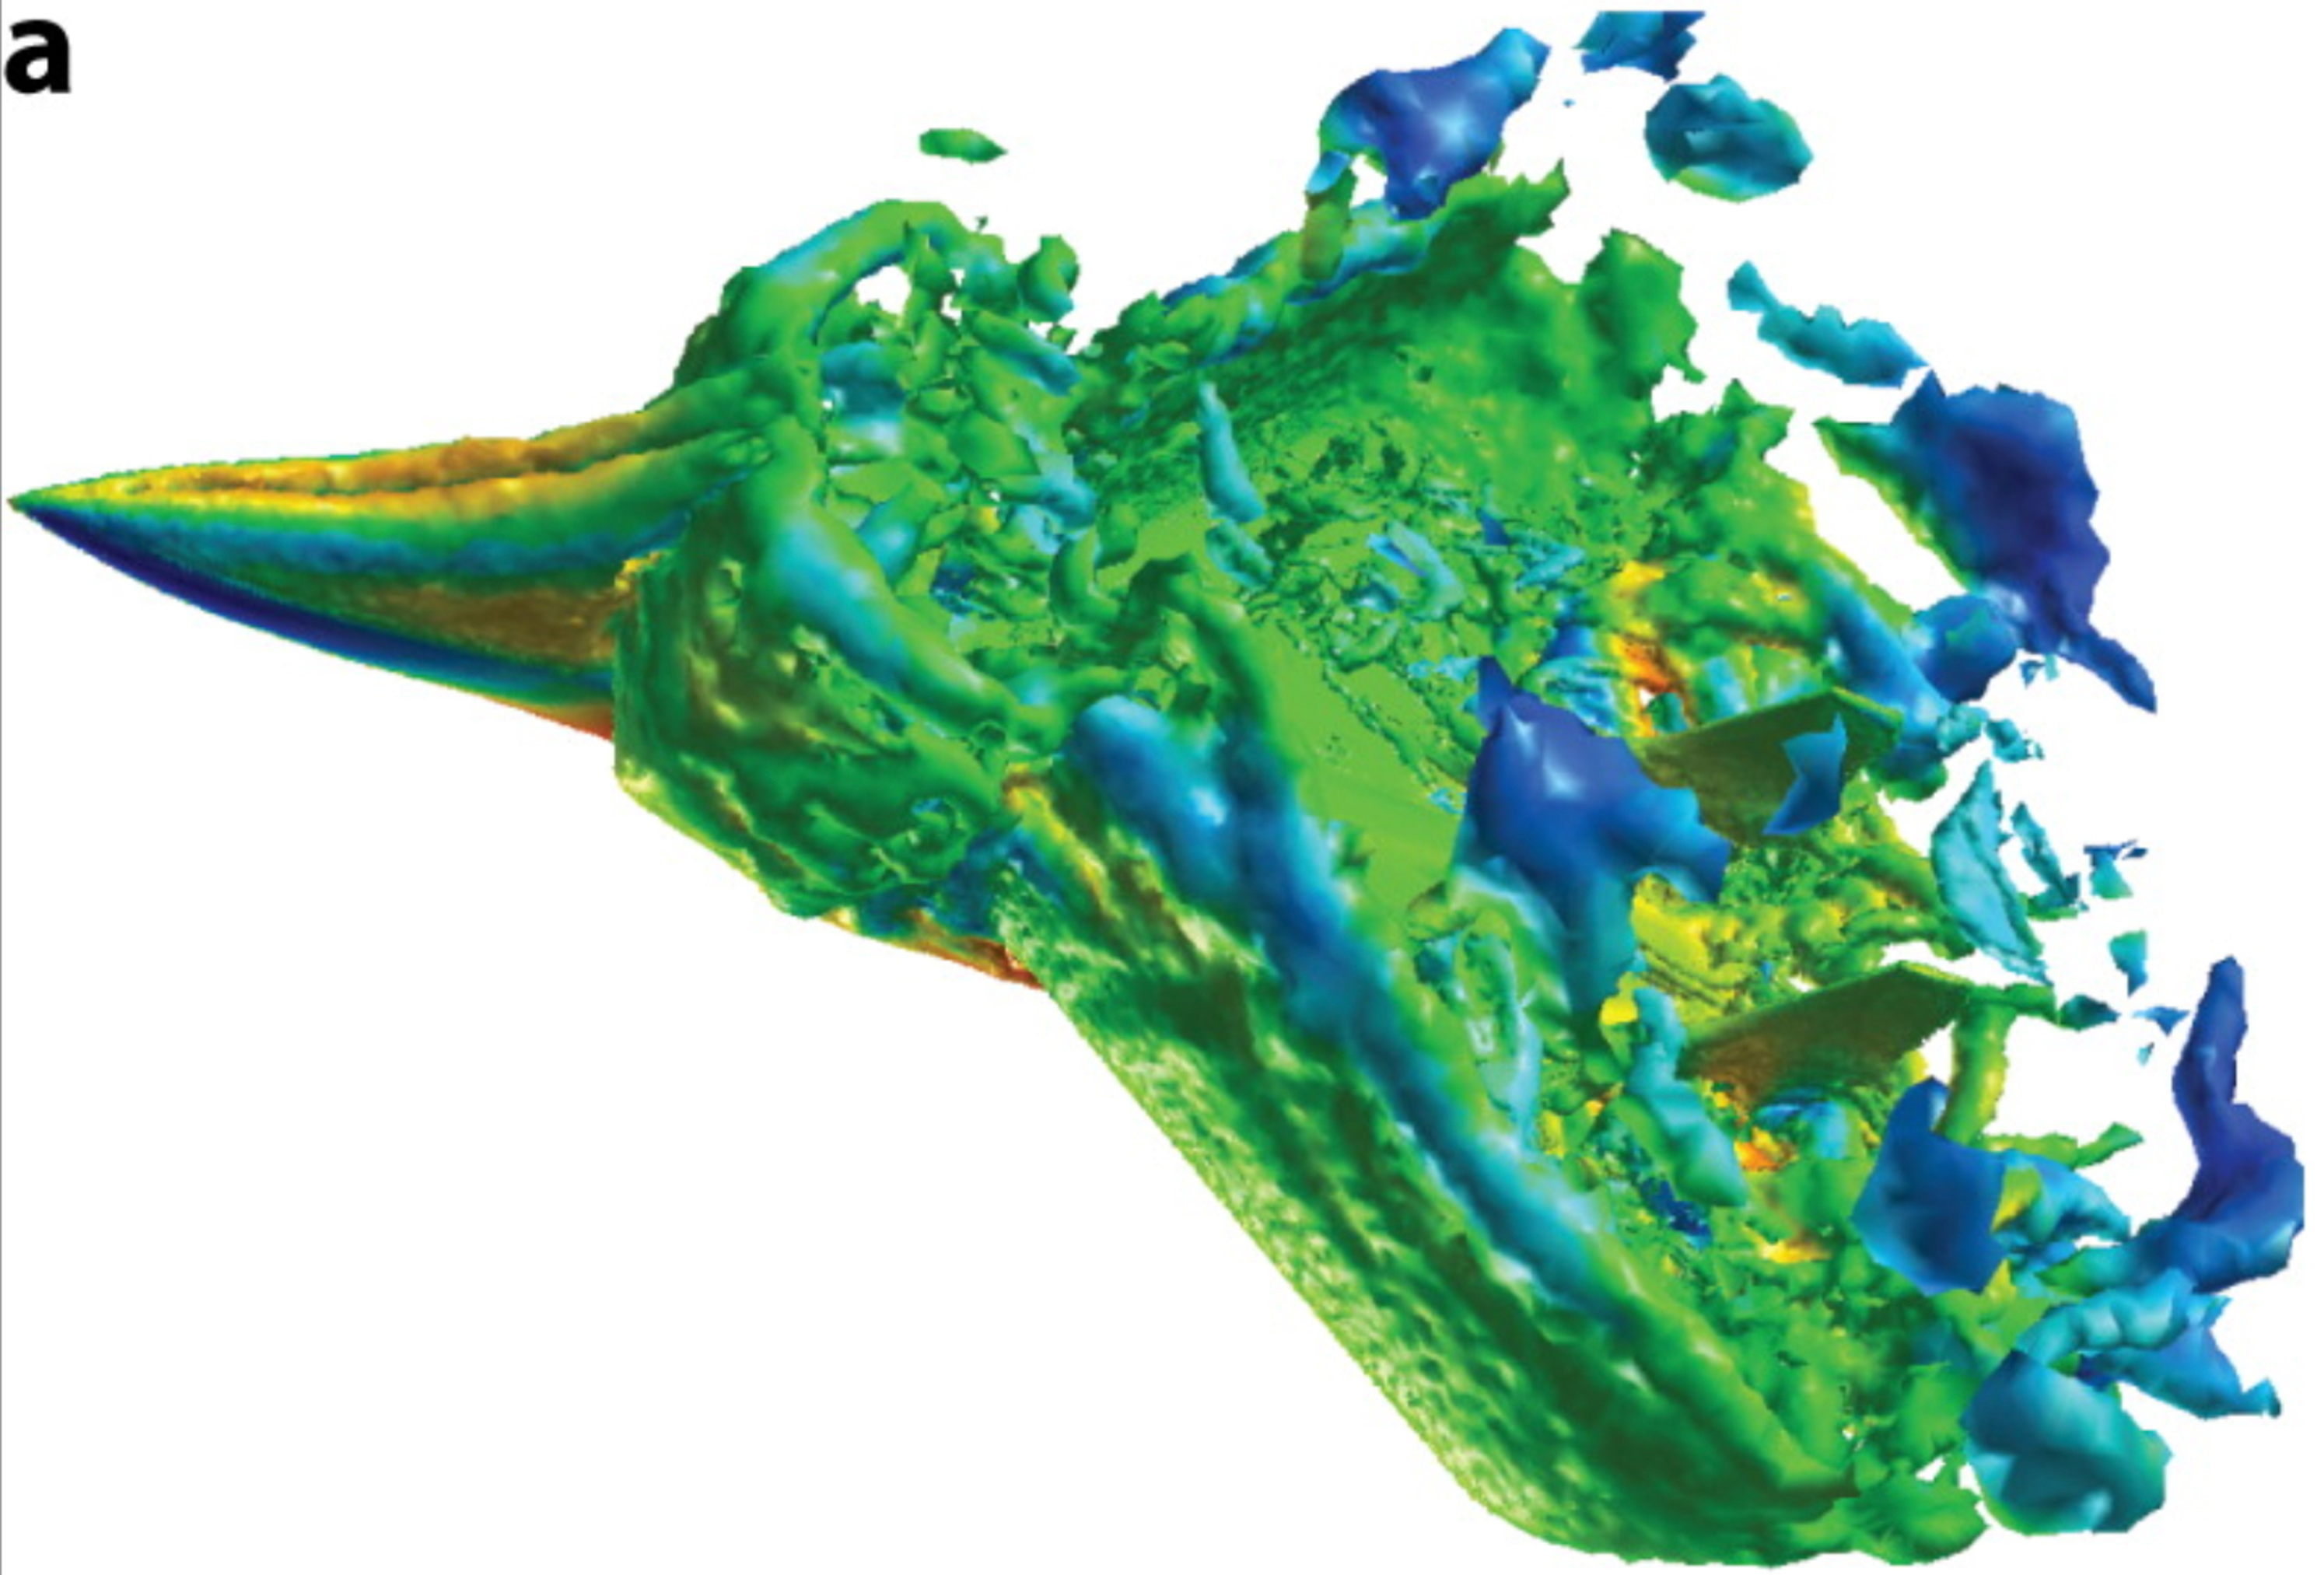
\includegraphics[width=0.45\textwidth]{Images/logan/spalart2009detachededdy_f15des.pdf}
\caption{ F-15 DES grid (left) \cite{forsythe2004detachededdy} vorticity isocontours (right) \cite{spalart2009detachededdy} }
\label{fig:f15des}
\end{center}
\end{figure}
%%\vspace{-2em}



%%% CAR DES
%%\vspace{-2em}
% \begin{figure}[htb]
\begin{figure}[H]
\begin{center}
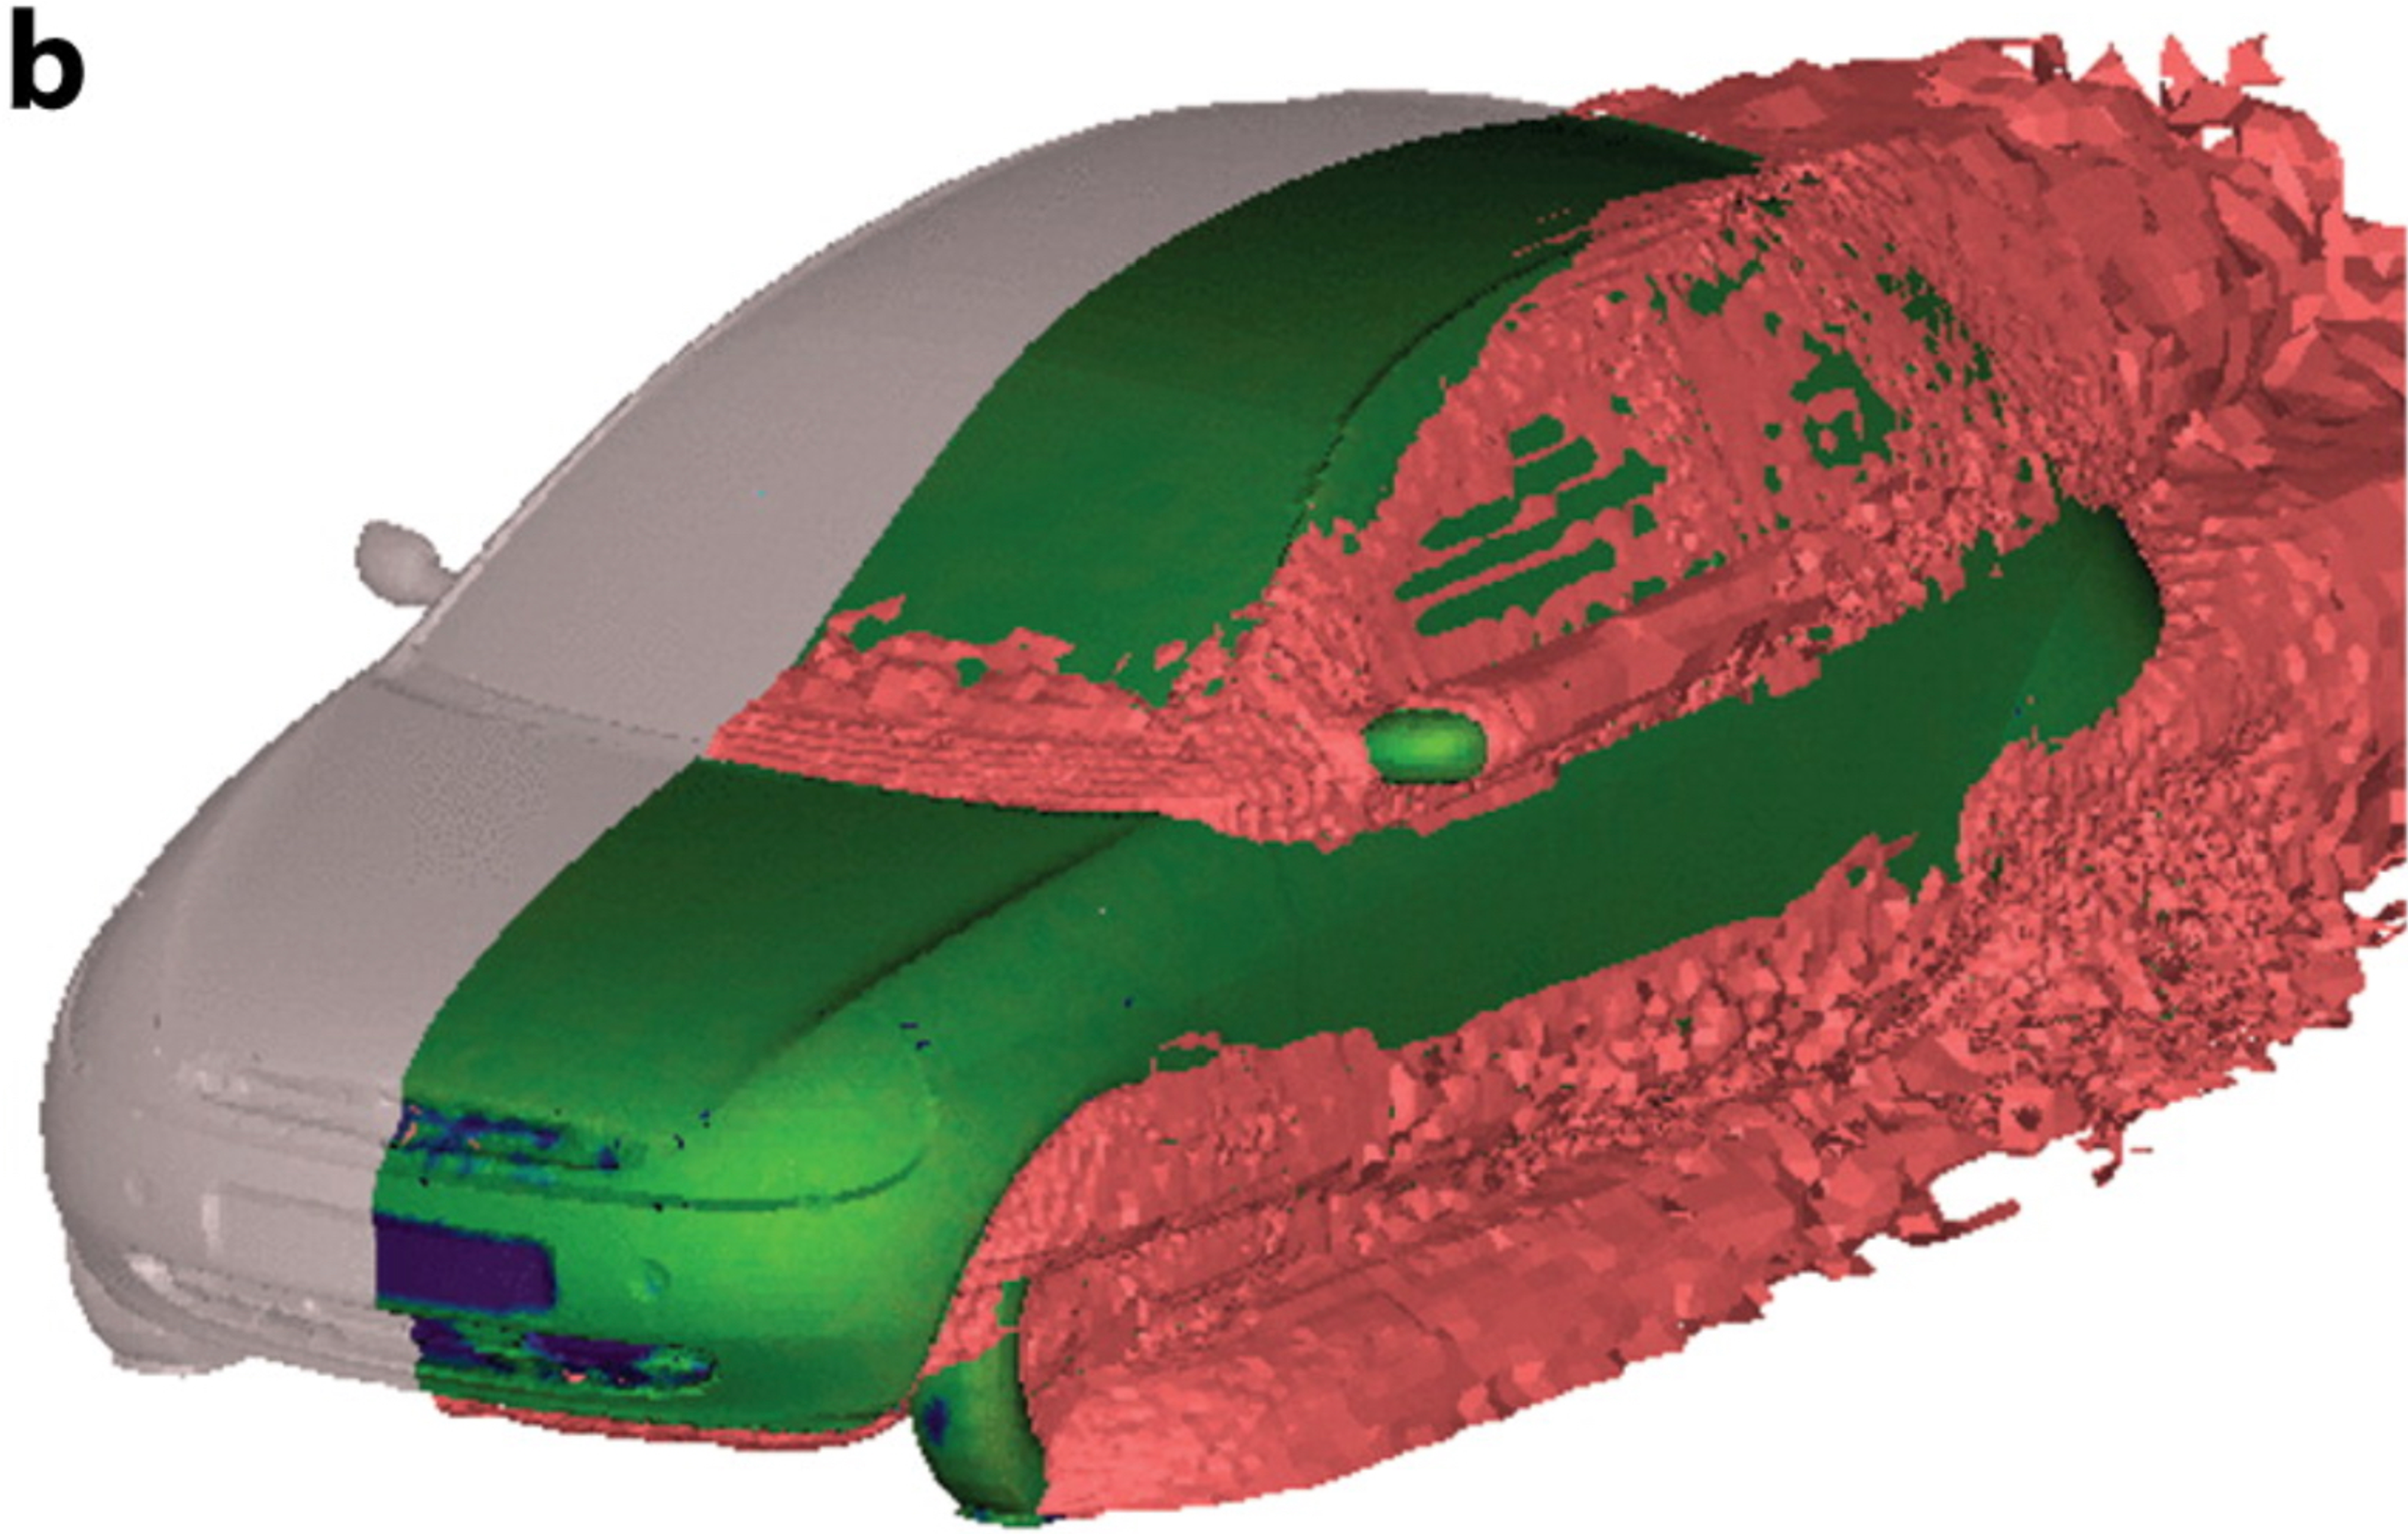
\includegraphics[width=0.5\textwidth]{Images/logan/spalart2009detachededdy_carDES.pdf}
\caption{ car DES isocontours \cite{mendonca2002towards} }
\label{fig:cardes}
\end{center}
\end{figure}
%%\vspace{-2em}














































%%%%%%%%%%%%%%%%%%%%%%%%%%%%%%%%%%%%%%%%%%%%%%%%%%%%%%%%%%%%%%%%%%%%%%%%
\section{Current State of Bluff-Body Turbulence Analysis} \label{sec:currentstate}
%%%%%%%%%%%%%%%%%%%%%%%%%%%%%%%%%%%%%%%%%%%%%%%%%%%%%%%%%%%%%%%%%%%%%%%%

\begin{itemize}
    \item Current State of Knowledge
    \item Remaining Challenges
\end{itemize}









%%%%%%%%%%%%%%%%%%%%%%%%%%%%%%%%%%%%%%%%%%%%%%%%%%%%%%%%%%%%%%%%%%%%%%%%
\subsection{Experimental Methods} \label{subsec:currentstateexperimental}

\textcolor{red}{\emph{FZ}}


%%%%%%%%%%%%%%%%%%%%%%%%%%%%%%%%%%%%%%%%%%%%%%%%%%%%%%%%%%%%%%%%%%%%%%%%
\subsection{Computational Methods} \label{subsec:currentstatecomputational}



\begin{itemize}
    \item Current State of Knowledge
    \item Remaining Challenges
    \item des GIS and order of accuracy
\end{itemize}



spalart table of methodology readiness




%%% GRID INDUCED SEPARATION FROM DES
%%\vspace{-2em}
% \begin{figure}[htb]
\begin{figure}[H]
\begin{center}
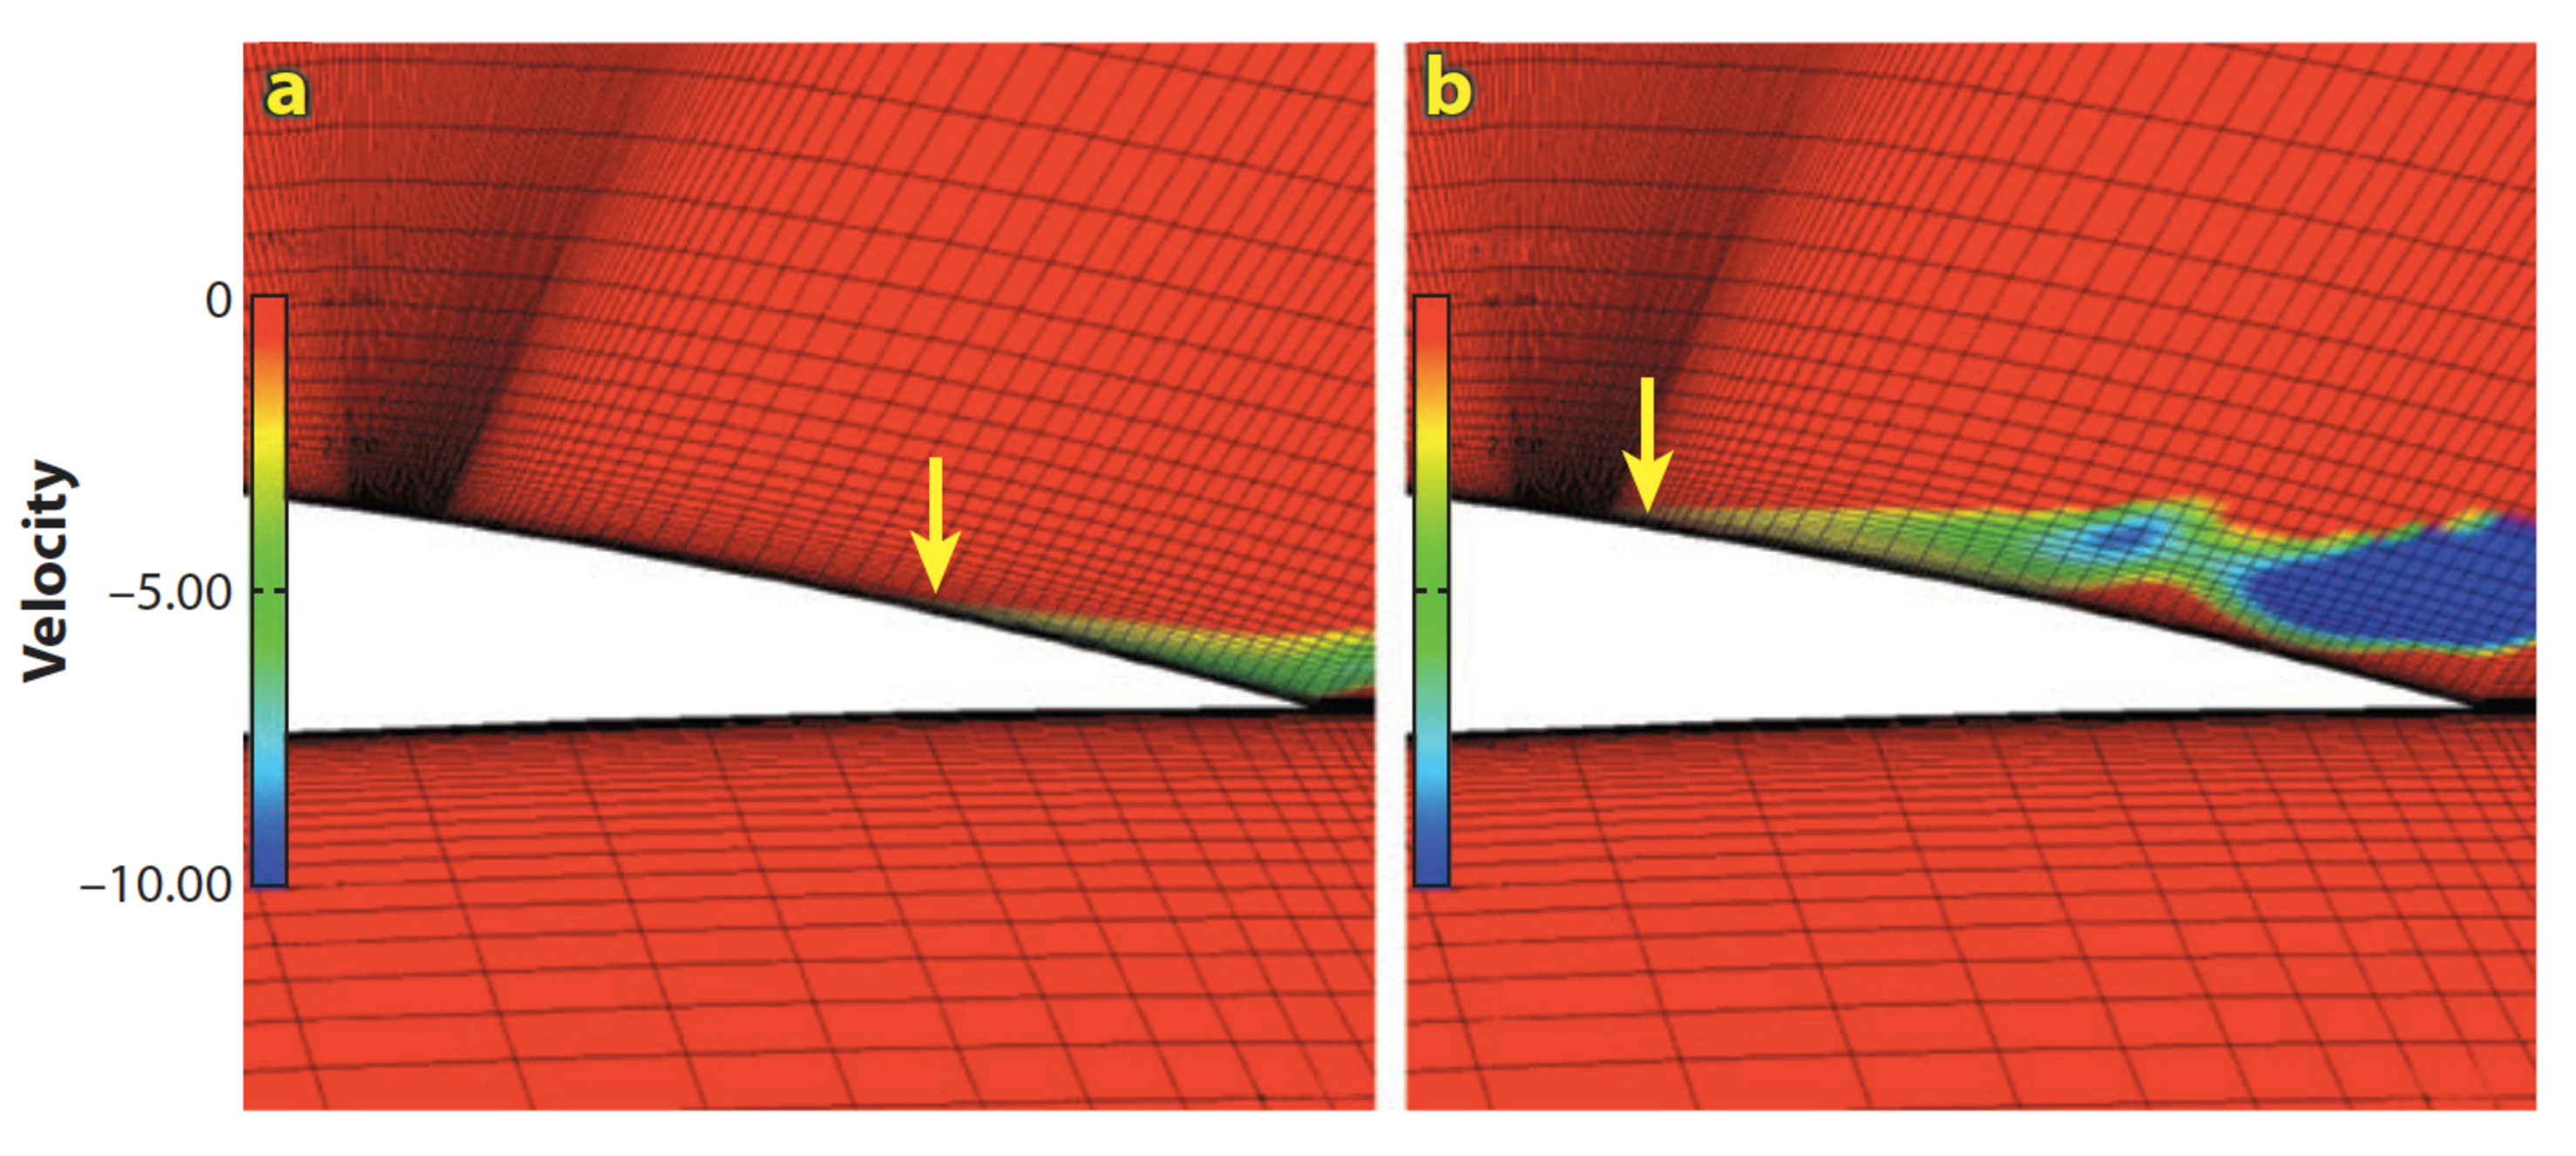
\includegraphics[width=0.6\textwidth]{Images/logan/spalart2009detachededdy_GridInducedSeparation.pdf}
\caption{ Example of DES grid induced separation from \cite{spalart2009detachededdy}, source: \cite{menter2004adaptation} }
\label{fig:desgridinducedseparation}
\end{center}
\end{figure}
%%\vspace{-2em}

Vorticity contours over an airfoil: (a) Reynolds-averaged Navier-Stokes and (b) detached-eddy simulation.
Arrows indicate separation. Figure taken from Menter \& Kuntz 2002.

Potential con of using DES. EXPLAIN HOW GRID INDUCED SEPARATION WORKS.







%%% GOLF BALL DNS
%%\vspace{-2em}
% \begin{figure}[htb]
\begin{figure}[H]
\begin{center}
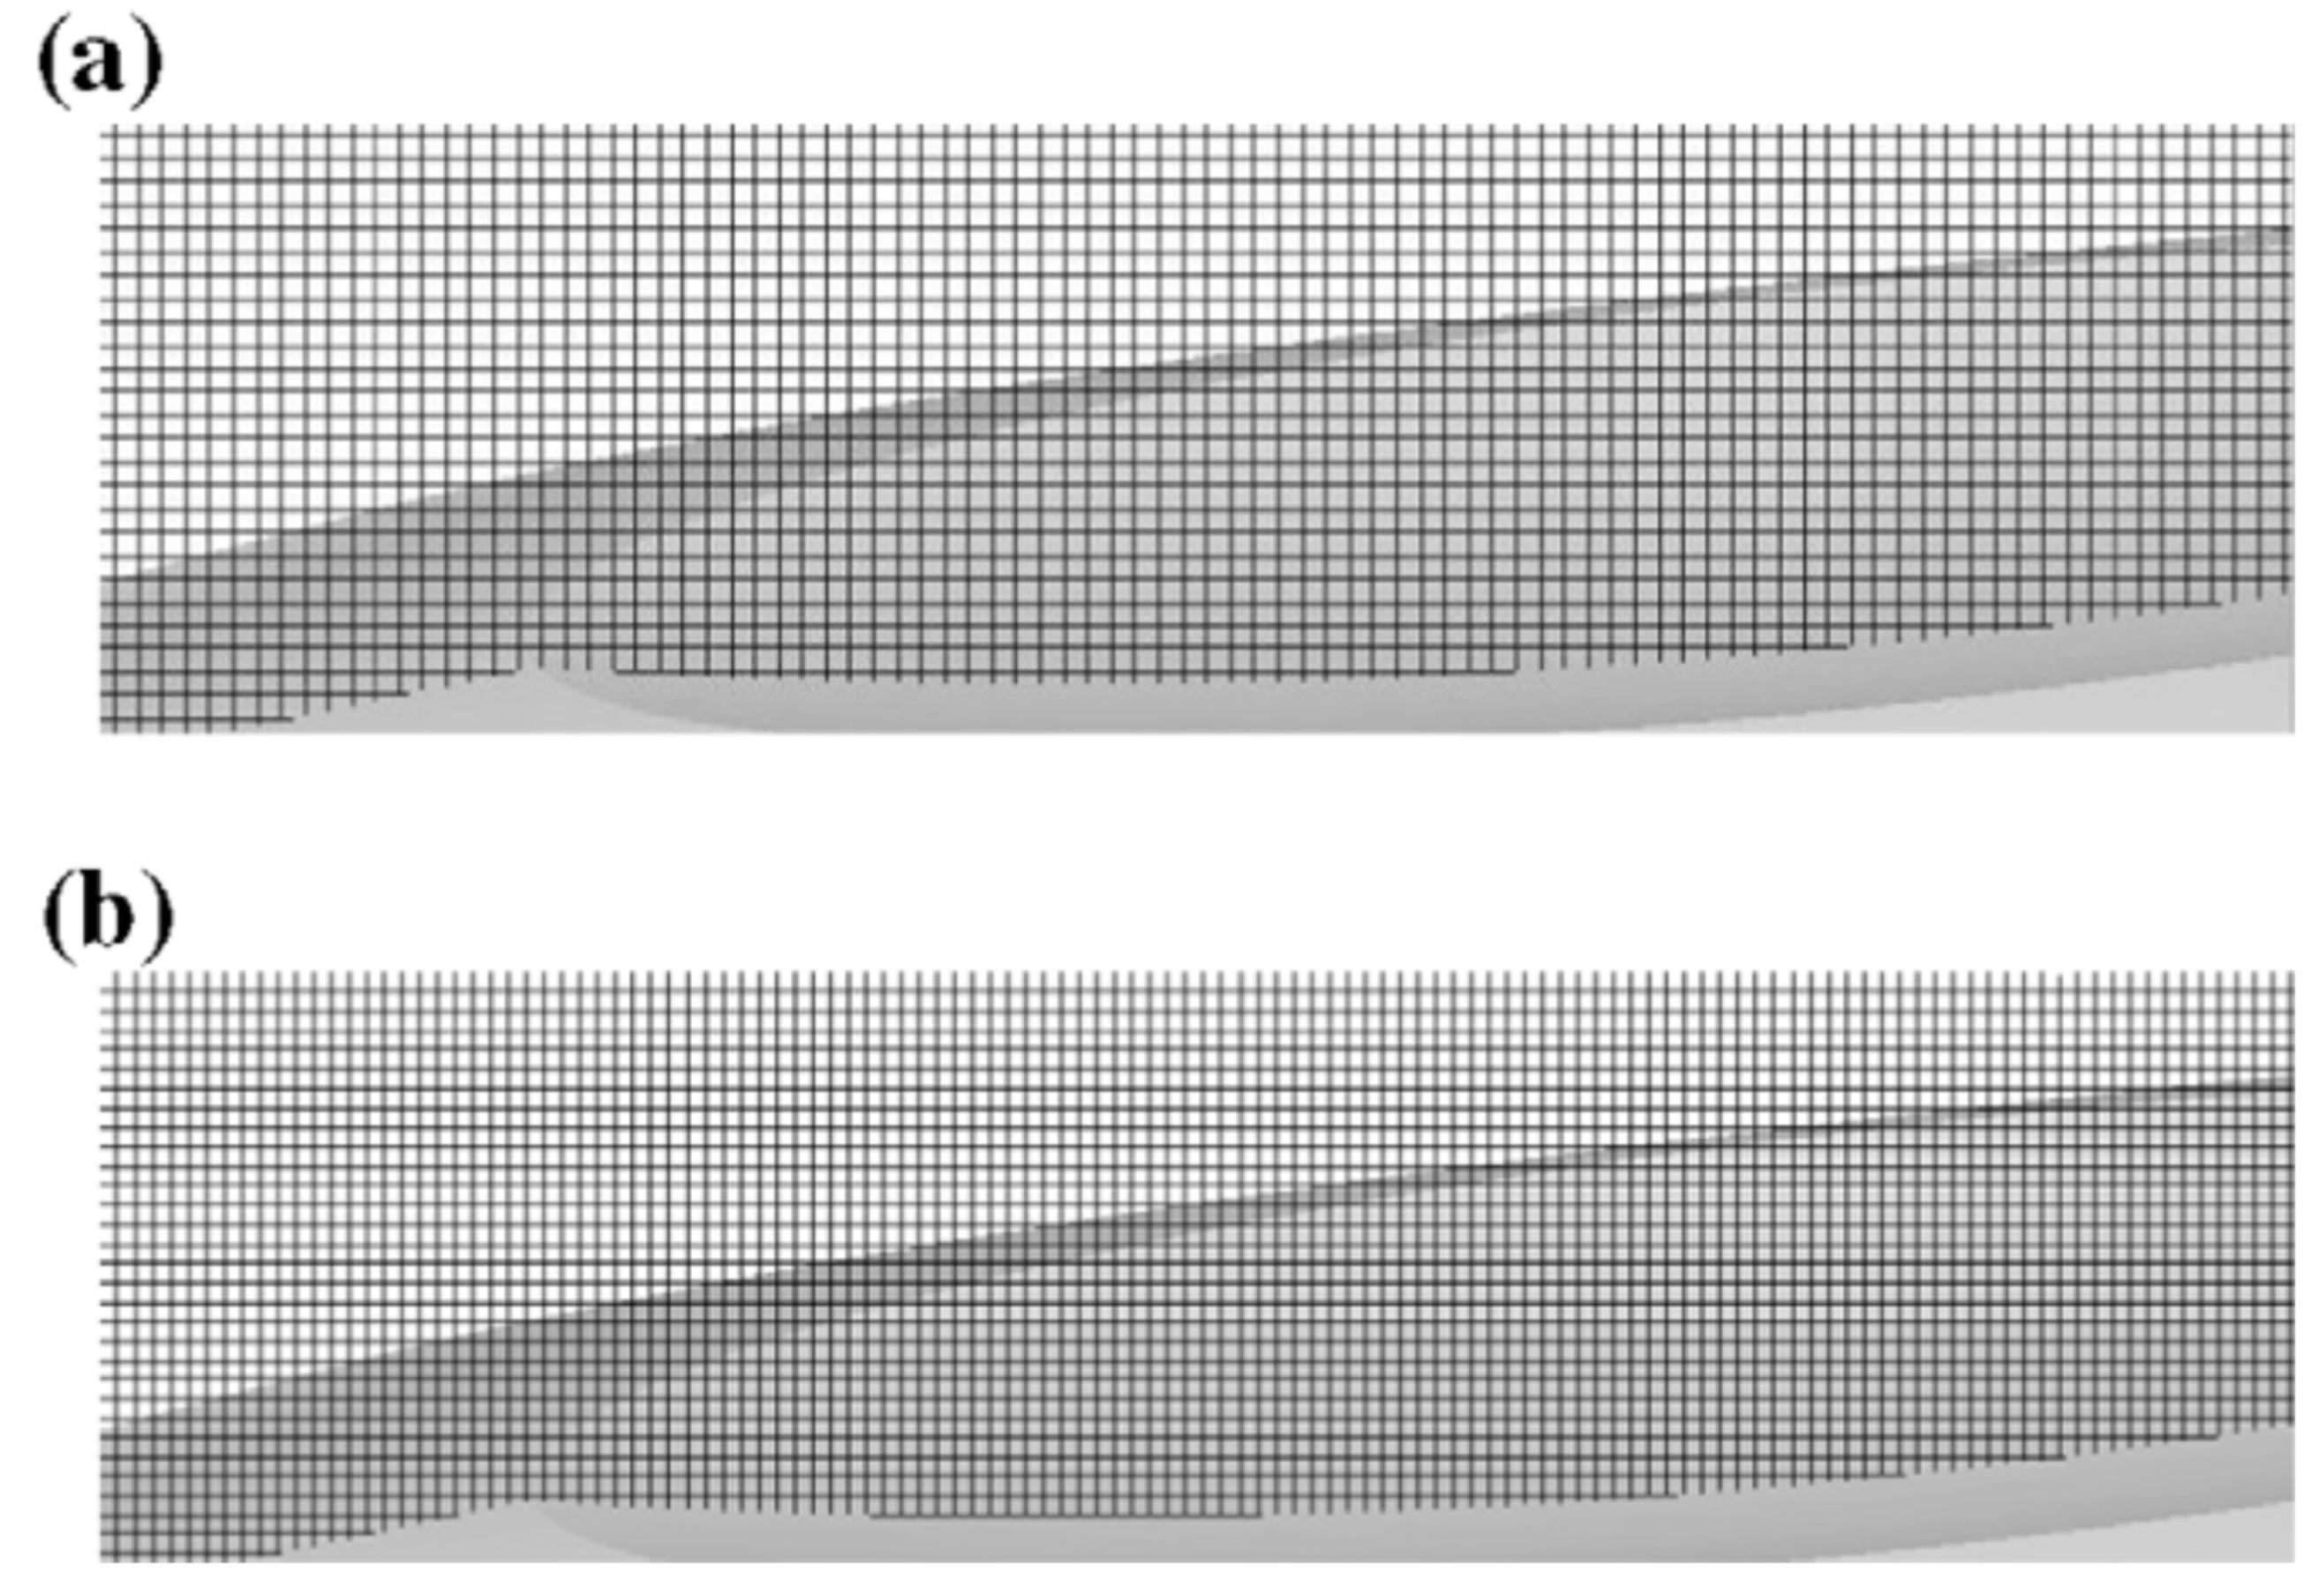
\includegraphics[width=0.45\textwidth]{Images/logan/smith2010numerical_golfballgrid.pdf}
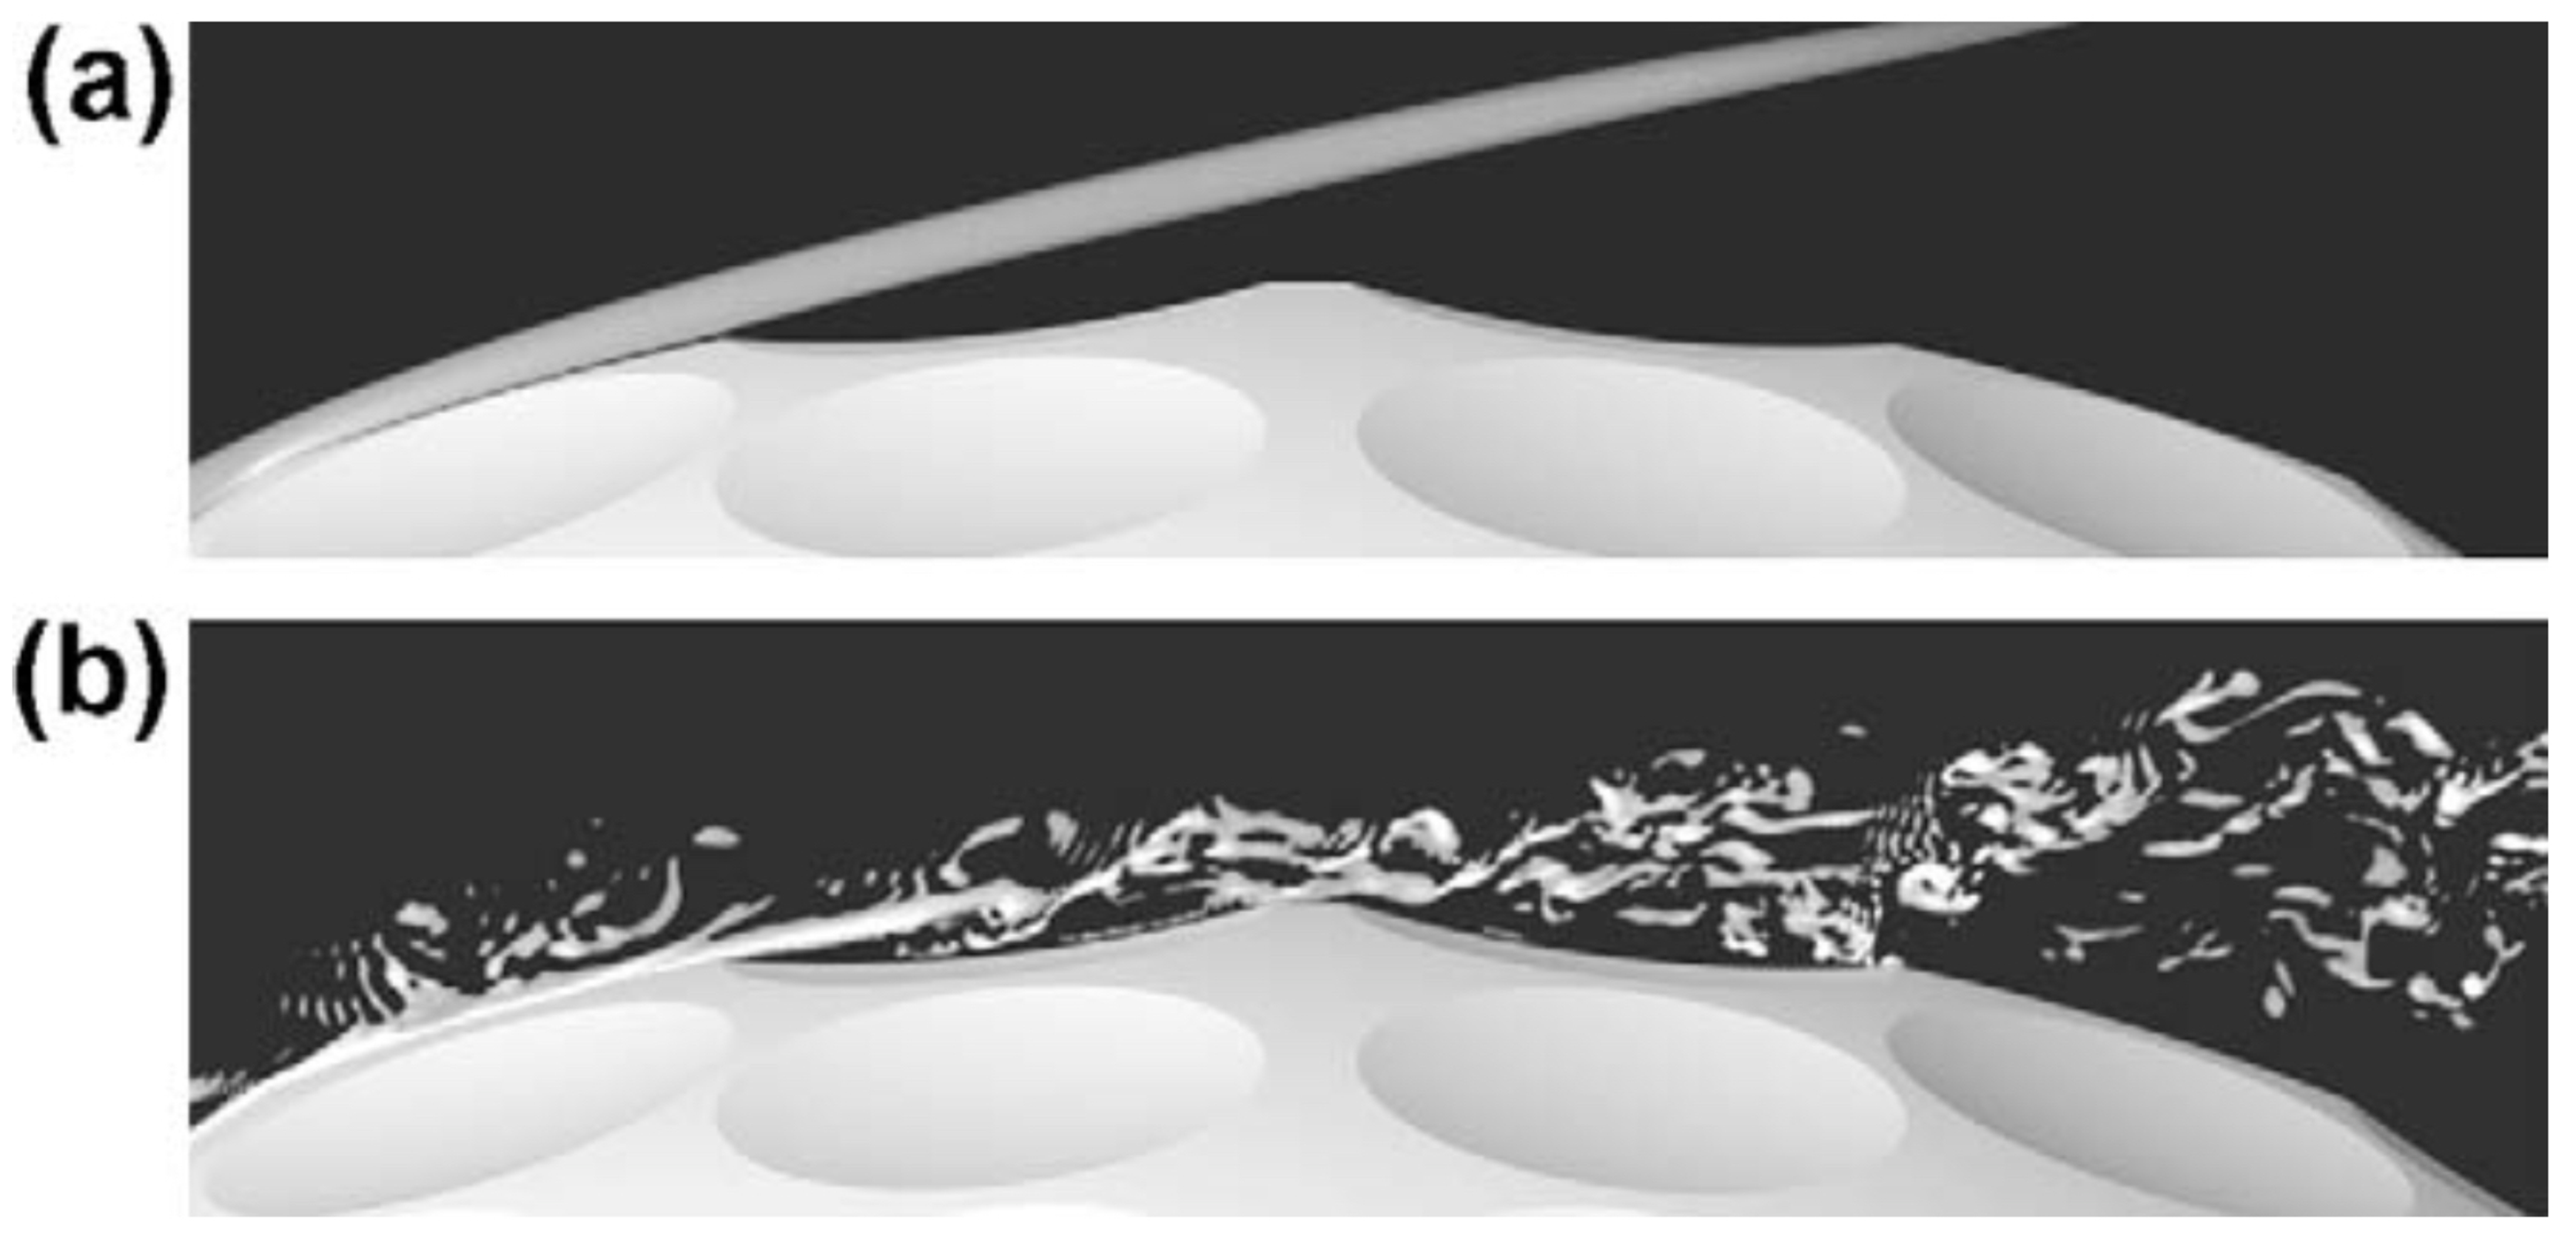
\includegraphics[width=0.45\textwidth]{Images/logan/smith2010numerical_golfballvorticity.pdf}
\caption{ DNS non-rotating golf ball with dimples grid (left) vorticity (right) \cite{smith2010numerical} }
\label{fig:dnsgolfball}
\end{center}
\end{figure}
%%\vspace{-2em}


Example grid resolution in a dimple near 84° (measured from the stagnation point at the front of the golf ball). (a) Re = 2.5   104; (b) Re = 1.1   105.

Contours of azimuthal vorticity. (a) Re = 2.5   104; (b) Re = 1.1   105

NOTE: Recall sphere example from Spalart review and say that this is the analogous DNS experiment to his DES

%%\vspace{-2em}
% \begin{figure}[htb]
\begin{figure}[H]
\begin{center}
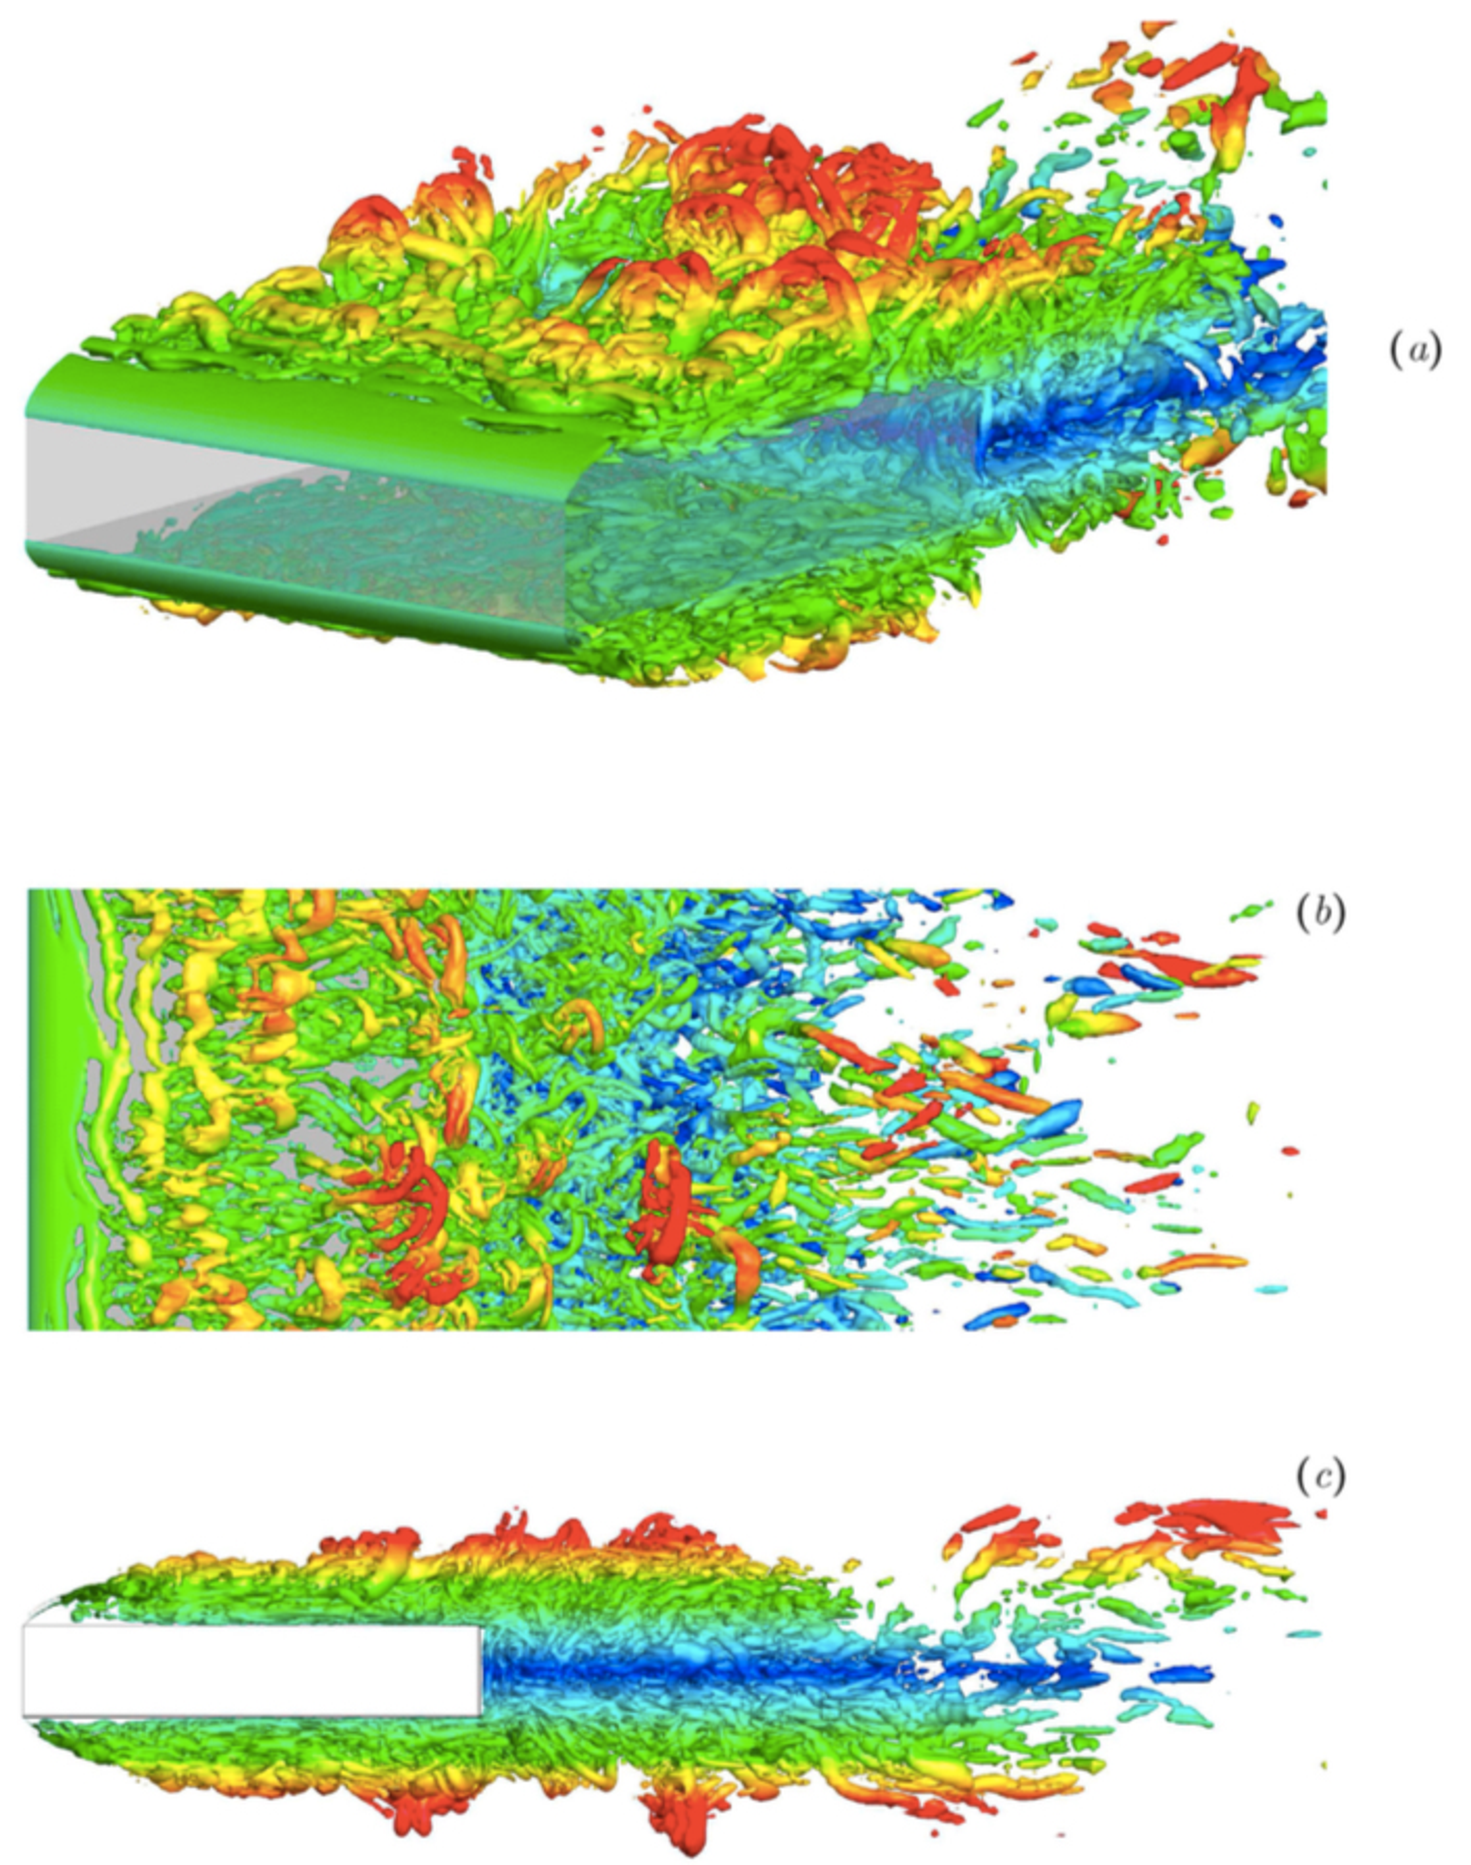
\includegraphics[width=0.5\textwidth]{Images/logan/cimarelli2018direct_vorticity.pdf}
\caption{ DNS square cylinder vorticity contours Re=3000 \cite{cimarelli2018direct} }
\label{fig:dnsRectCylPressure}
\end{center}
\end{figure}
%%\vspace{-2em}

Fig. 10. Instantaneous isosurfaces of $\lambda_2=-2$ colored with $y$. Perspective, top and lateral views in (a), (b) and (c) plots, respectively.







\textcolor{red}{\emph{LH}}

\begin{itemize}
    \item \underline{Brief} turbulence model description
    \begin{itemize}
        \item RANS vs URANS
        \item DNS
        \item LES (uses DNS) and DES (=Hybrid RANS/LES)
    \end{itemize}
    \item Compare turbulence model performance for sphere/cylinder
    \begin{itemize}
        \item DES > URANS > RANS
        \item DES = functional LES
        \item SAS vs DES?
        \item DNS: limited Re
    \end{itemize}
    \item Shortcomings of each model (and how to address them)
    \begin{itemize}
        \item URANS
        \item DES: only good at sharp separation
        \begin{itemize}
            \item ``An order of accuracy has not even been proposed for a simulation using both modes within DES'' -Spalart about hybrid method
            \item grid induced separation (maybe not an issue for bluff bodies)
            \item DES can default to RANS if grid adaptation misses a shear layer
            \item more computational cost than RANS
    \end{itemize}
    \end{itemize}
    \item Advanced geometries
    \begin{itemize}
        \item f-15
        \item car
        \item building
        \item capsule
        \item chute, landing gear, helicopter, wind turbine
    \end{itemize}
\end{itemize}


LIST ALL FIGURES HERE, REORDER AND DESCRIBE LATER







% %%% LES VS RANS CYLINDER
% %%\vspace{-2em}
% % \begin{figure}[htb]
% \begin{figure}[H]
% \begin{center}
% 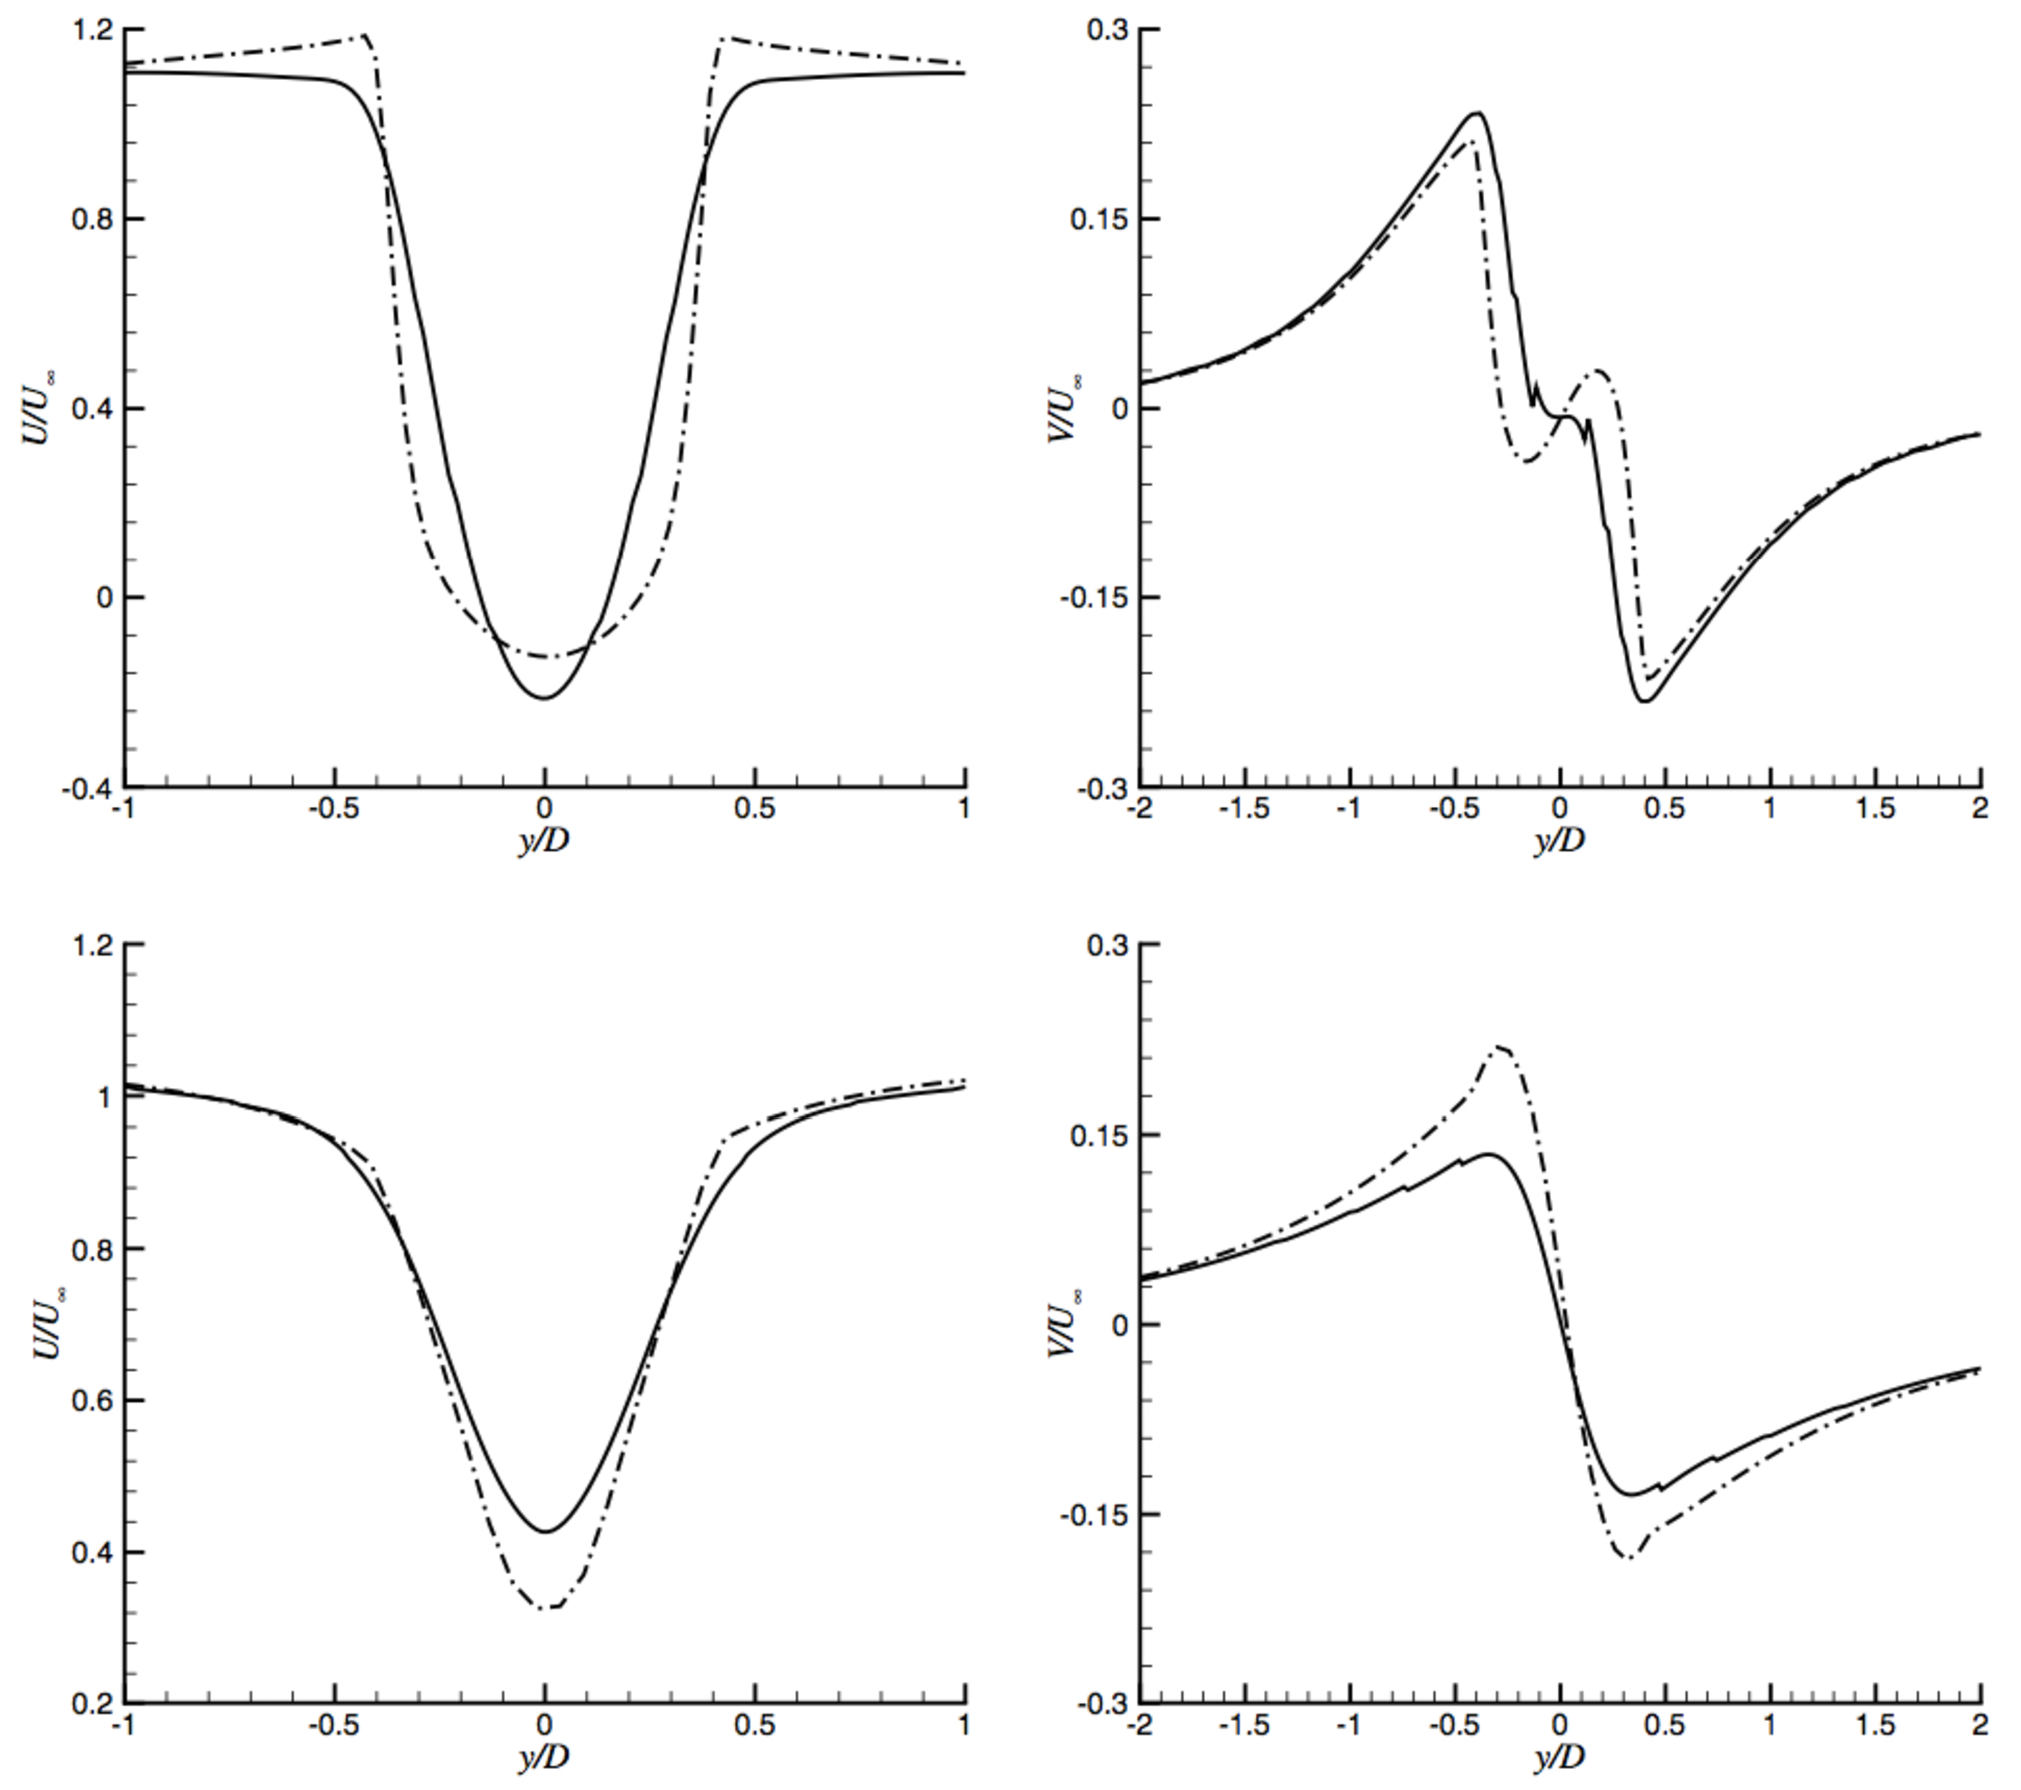
\includegraphics[width=0.5\textwidth]{Images/logan/catalano_2003numerical_VelocityProfiles.pdf}
% \caption{ cylinder les vs urans velocity profiles \cite{catalano2003numerical} }
% \label{fig:lesvsuranscylindervelprofile}
% \end{center}
% \end{figure}
% %%\vspace{-2em}

% Fig. 6. Mean streamwise and vertical velocities at x=D 1⁄4 0:75 (upper figures) and x=D 1⁄4 1:50 (lower figures): (—) LES; (– –) URANS



% %%%%%%%%%%%%%%%%%%%%%%%%%%%%%%%%%%%%%%%%%%%%%%%%%%%%%%%%%%%%

% %%% LES VS RANS CYLINDER GRID
% %%\vspace{-2em}
% % \begin{figure}[htb]
% \begin{figure}[H]
% \begin{center}
% 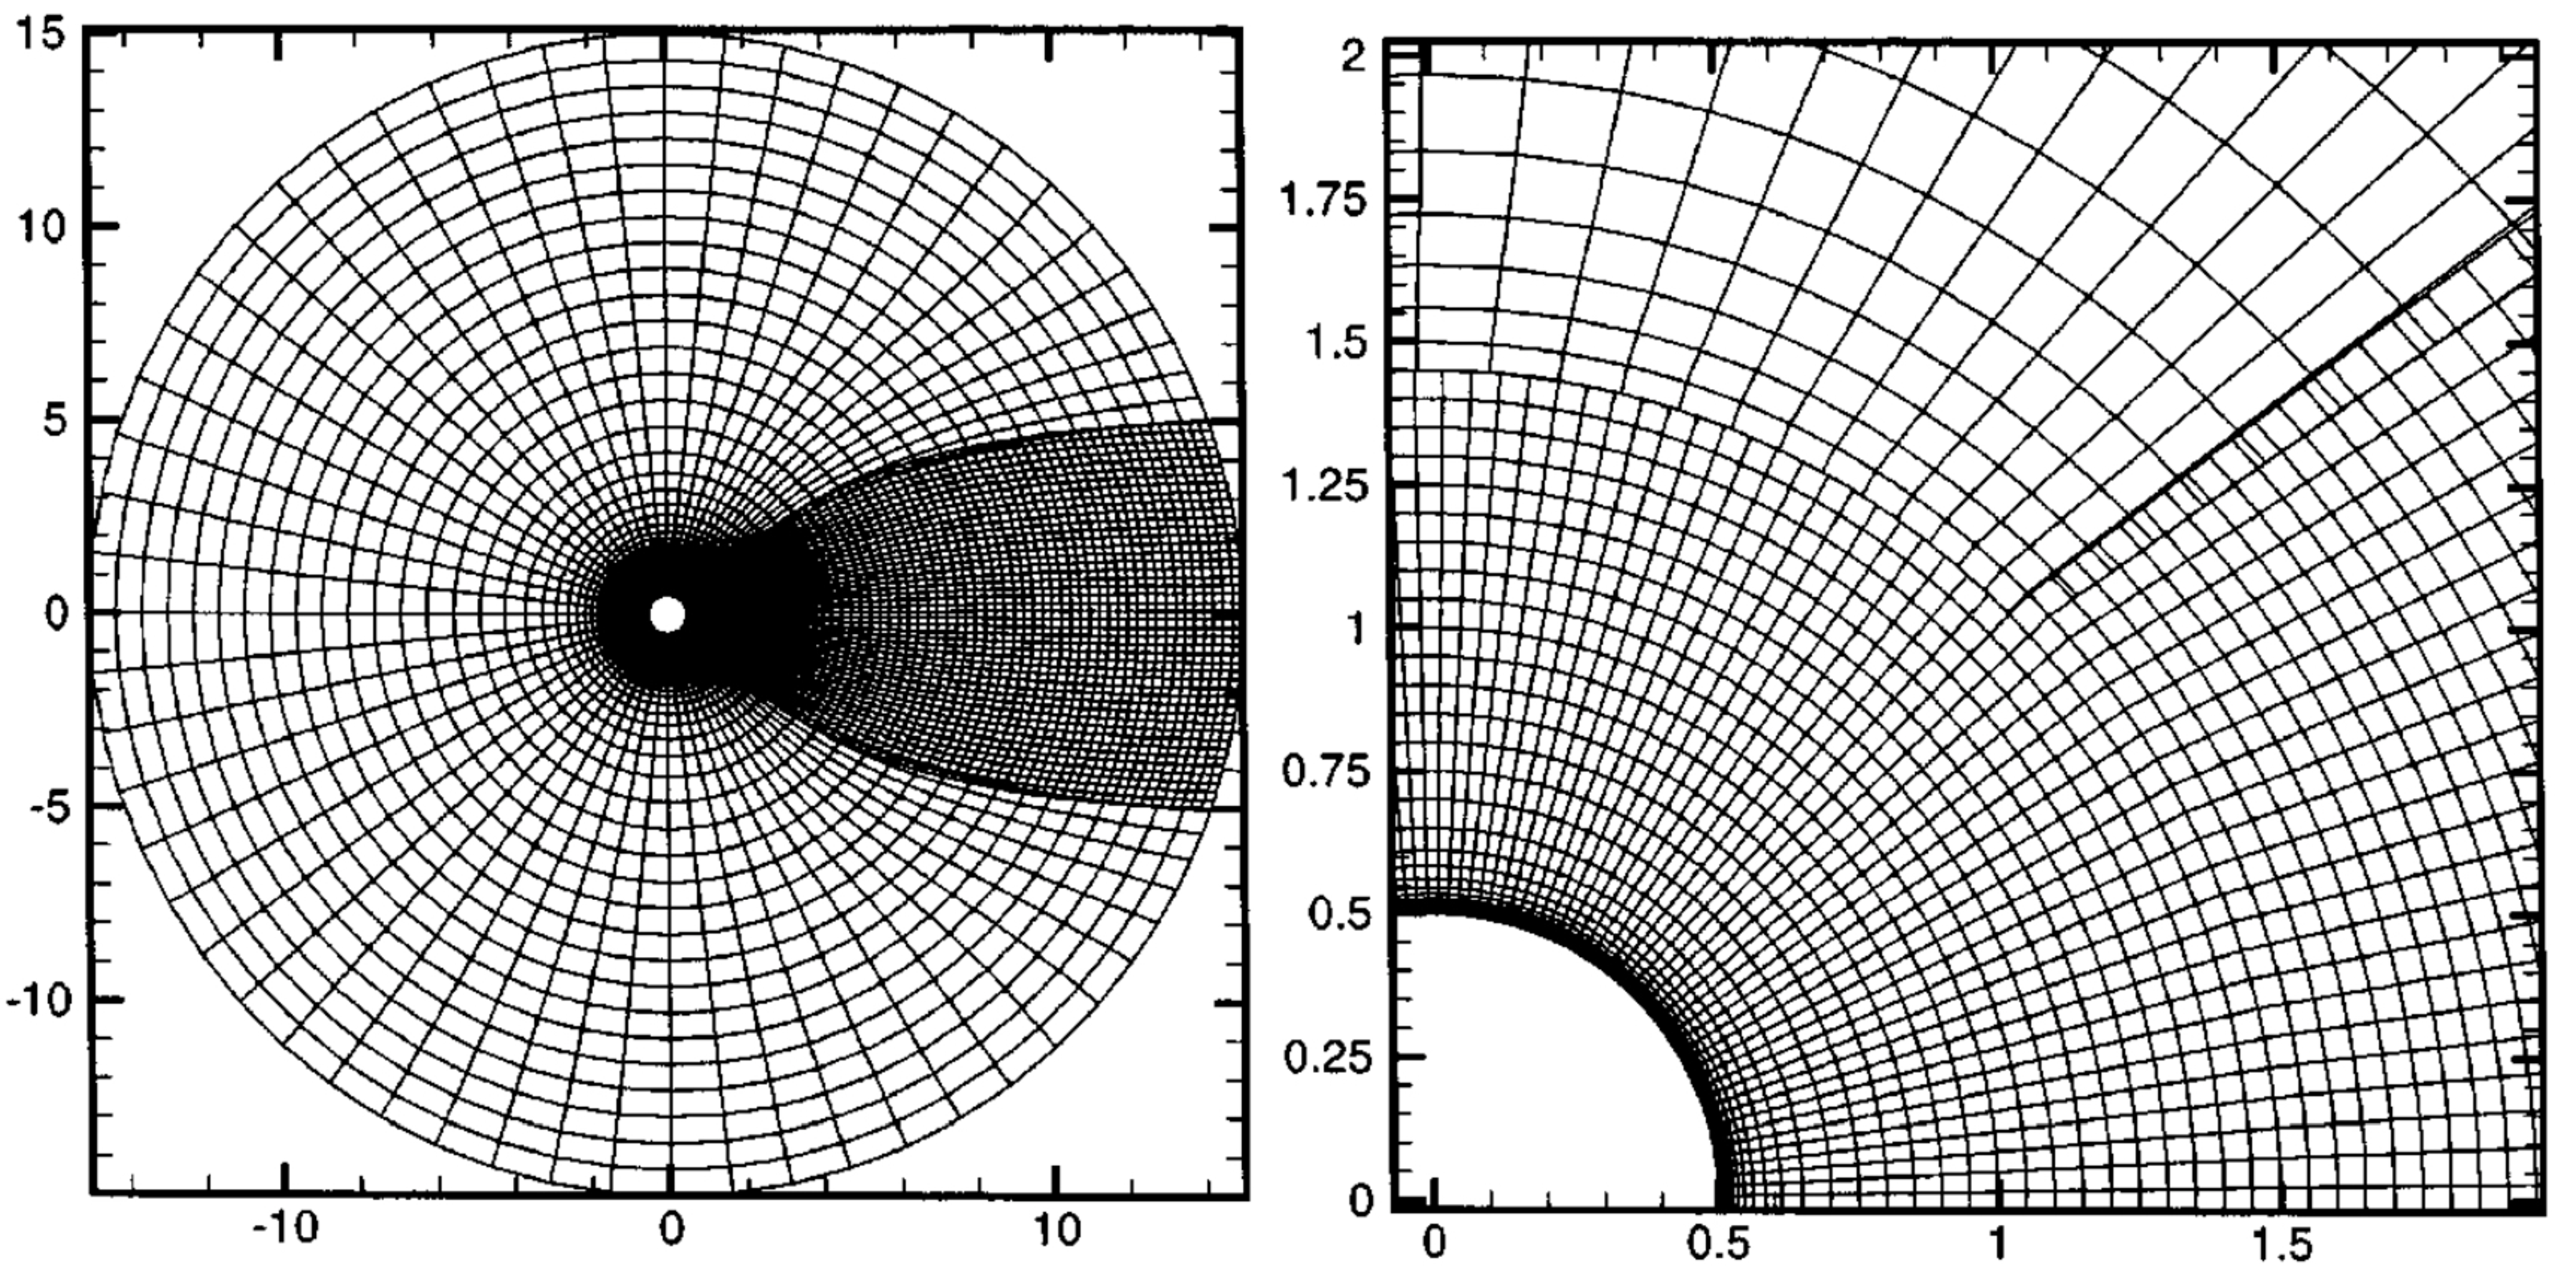
\includegraphics[width=0.5\textwidth]{Images/logan/travin2000detachededdy_grid.pdf}
% \caption{ cylinder les vs rans grid \cite{travin2000detachededdy} }
% \label{fig:lesvsranscylindergrid}
% \end{center}
% \end{figure}
% %%\vspace{-2em}

% Figure1. Medium computational grid, CaseTS2.Innerblock150×36,wakeblock74×36, outer block 59 × 30. The three blocks meet near x = 1.06, y = 1.03.  Grid for spalart cylinders.


% %%% LES VS RANS CYLINDER
% %%\vspace{-2em}
% % \begin{figure}[htb]
% \begin{figure}[H]
% \begin{center}
% 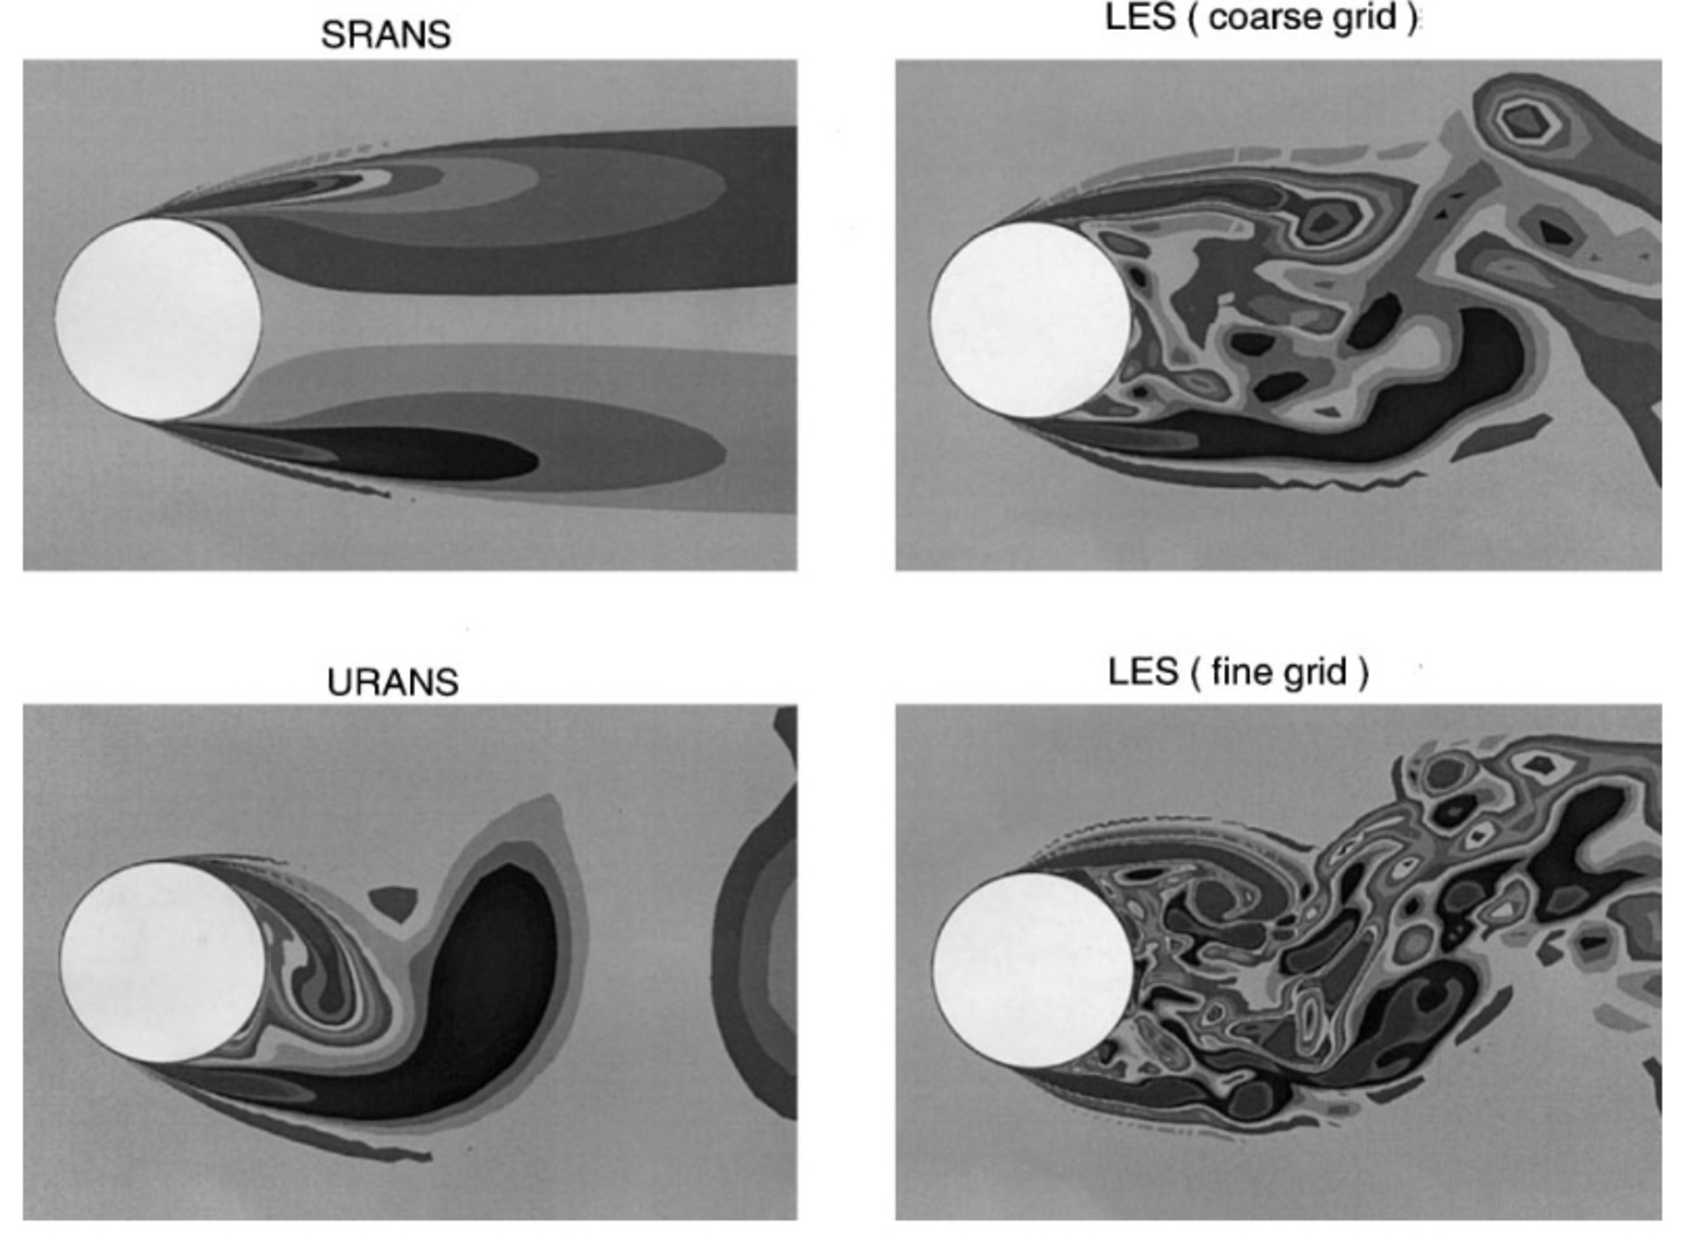
\includegraphics[width=0.5\textwidth]{Images/logan/spalart2000strategies_CylinderLESvsRANS.pdf}
% \caption{ cylinder les vs rans \cite{spalart2000strategies} }
% \label{fig:lesvsranscylinder}
% \end{center}
% \end{figure}
% %%\vspace{-2em}


% grid for LES shown above (actual simulations were DES)






%%%%%%%%%%%%%%%%%%%%%%%%%%%%%%%%%%%%%%%%%%%%%%%%%%%%%%%%%%%%


% %%% CURVE BACKSTEP VELOCITY PROFILE LES VS RANS
% %%\vspace{-2em}
% % \begin{figure}[htb]
% \begin{figure}[H]
% \begin{center}
% 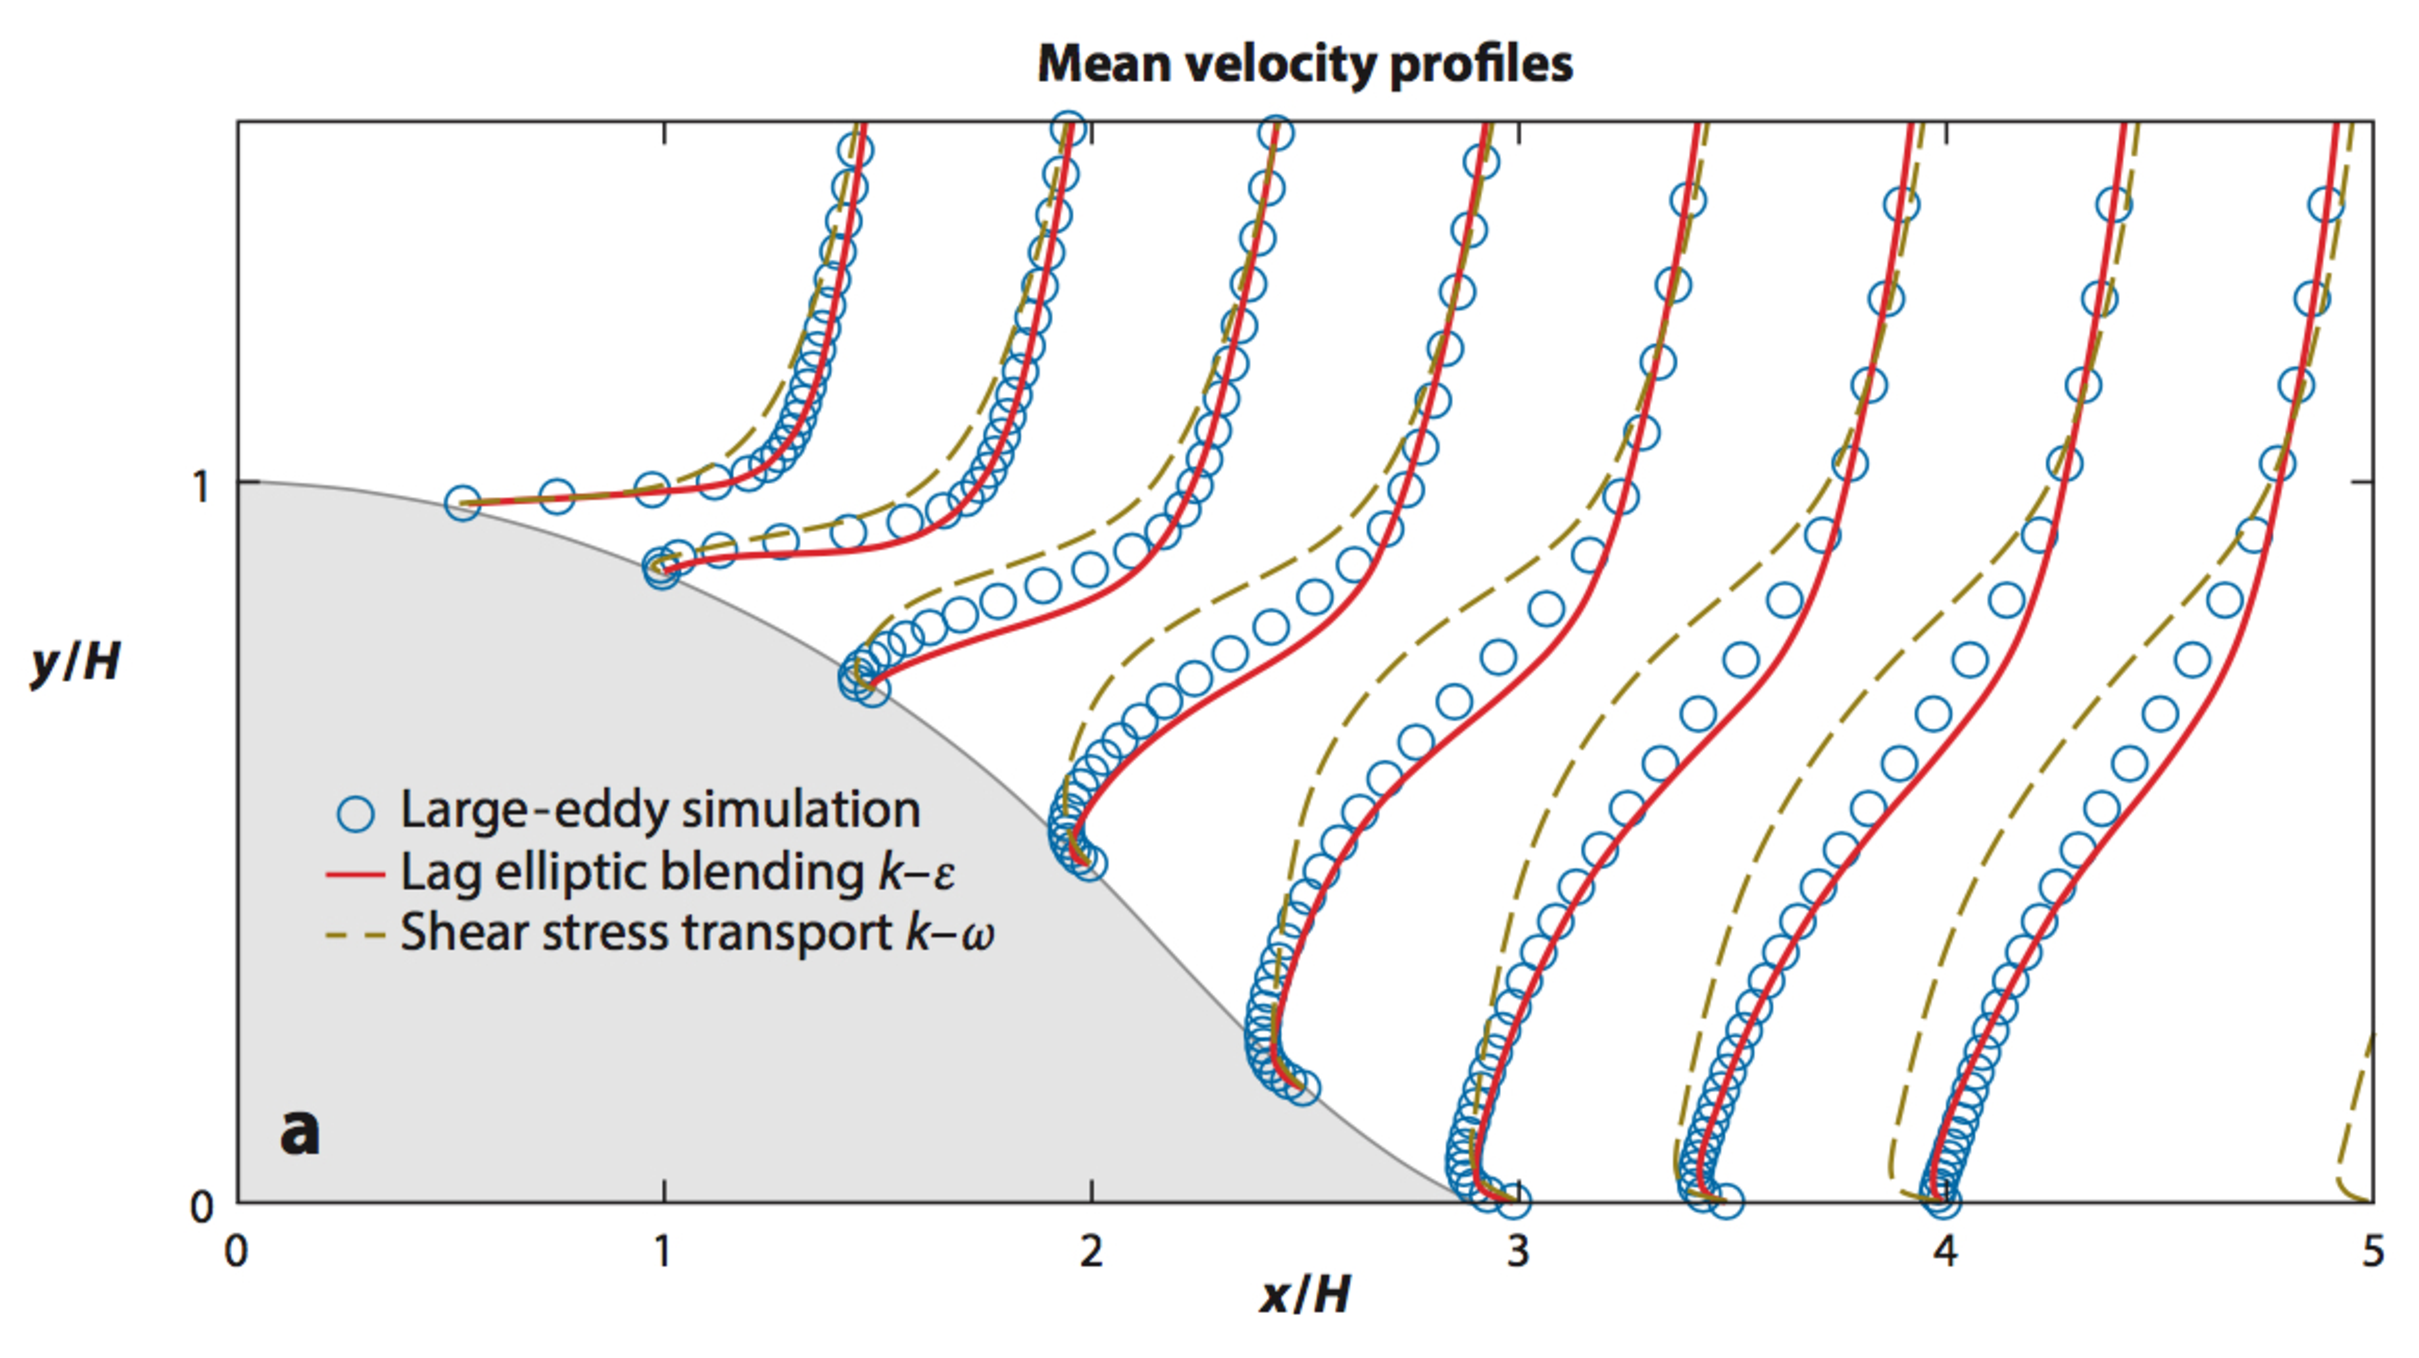
\includegraphics[width=0.5\textwidth]{Images/logan/durbin2018some_BackstepLESvsRANS.pdf}
% \caption{curve backstep velocity profile les vs rans \cite{durbin2018some}}
% \label{fig:lesvsransbackstep}
% \end{center}
% \end{figure}
% %%\vspace{-2em}










% %%% RECTANCULAR CYLINDER DNS
% %%\vspace{-2em}
% % \begin{figure}[htb]
% \begin{figure}[H]
% \begin{center}
% 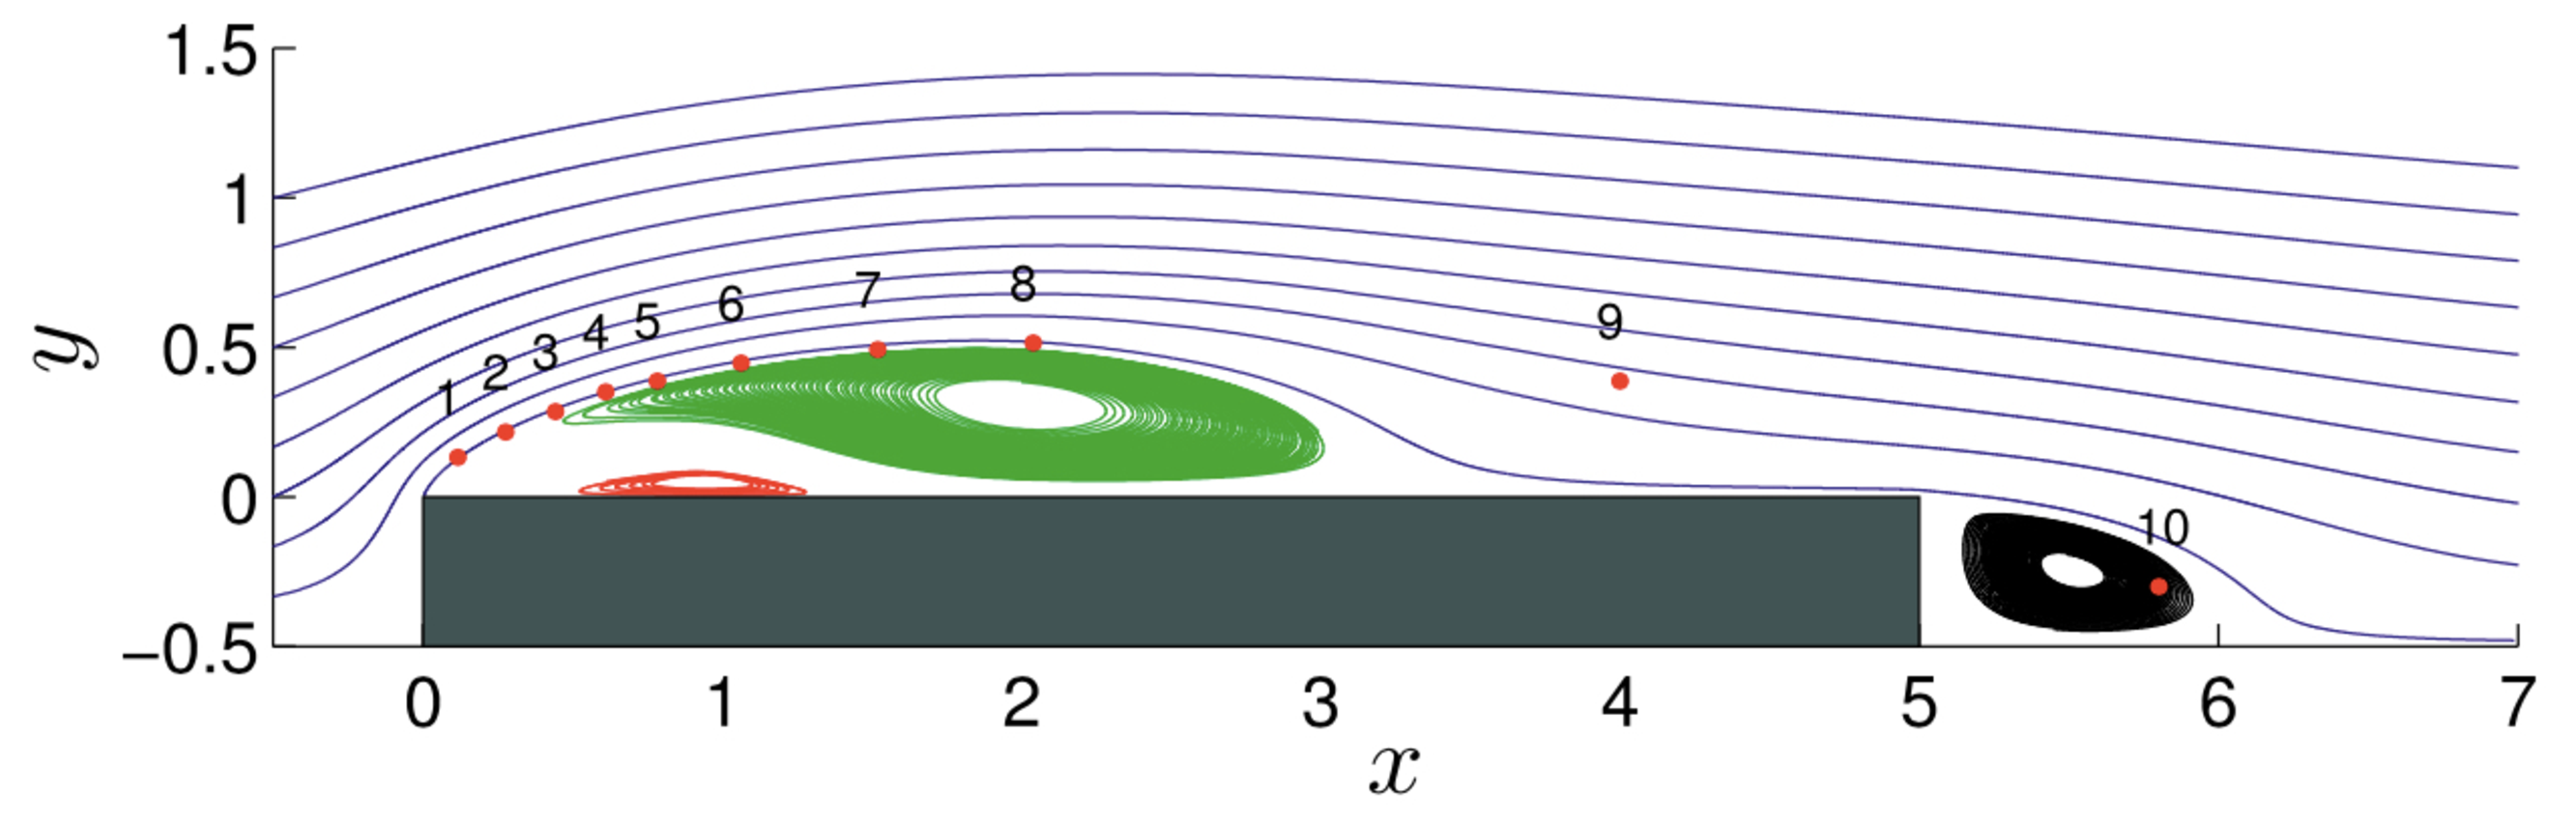
\includegraphics[width=0.45\textwidth]{Images/logan/cimarelli2018direct_vortices.pdf}
% \caption{ DNS square cylinder vortex locations Re=3000 \cite{cimarelli2018direct} }
% \label{fig:dnsRectCylVortices}
% \end{center}
% \end{figure}
% %%\vspace{-2em}


% Fig. 4. Streamlines of the mean velocity field (U,V) (x,y)  The green lines show the primary vortex, the red lines mark the secondary vortex and the black lines denote the wake vortex. The red dots denote the locations of the probes used for the computation of time spectra in section x5. (For interpretation of the references to color in this figure legend, the reader is referred to the Web version of this article.)

% %%\vspace{-2em}
% % \begin{figure}[htb]
% \begin{figure}[H]
% \begin{center}
% 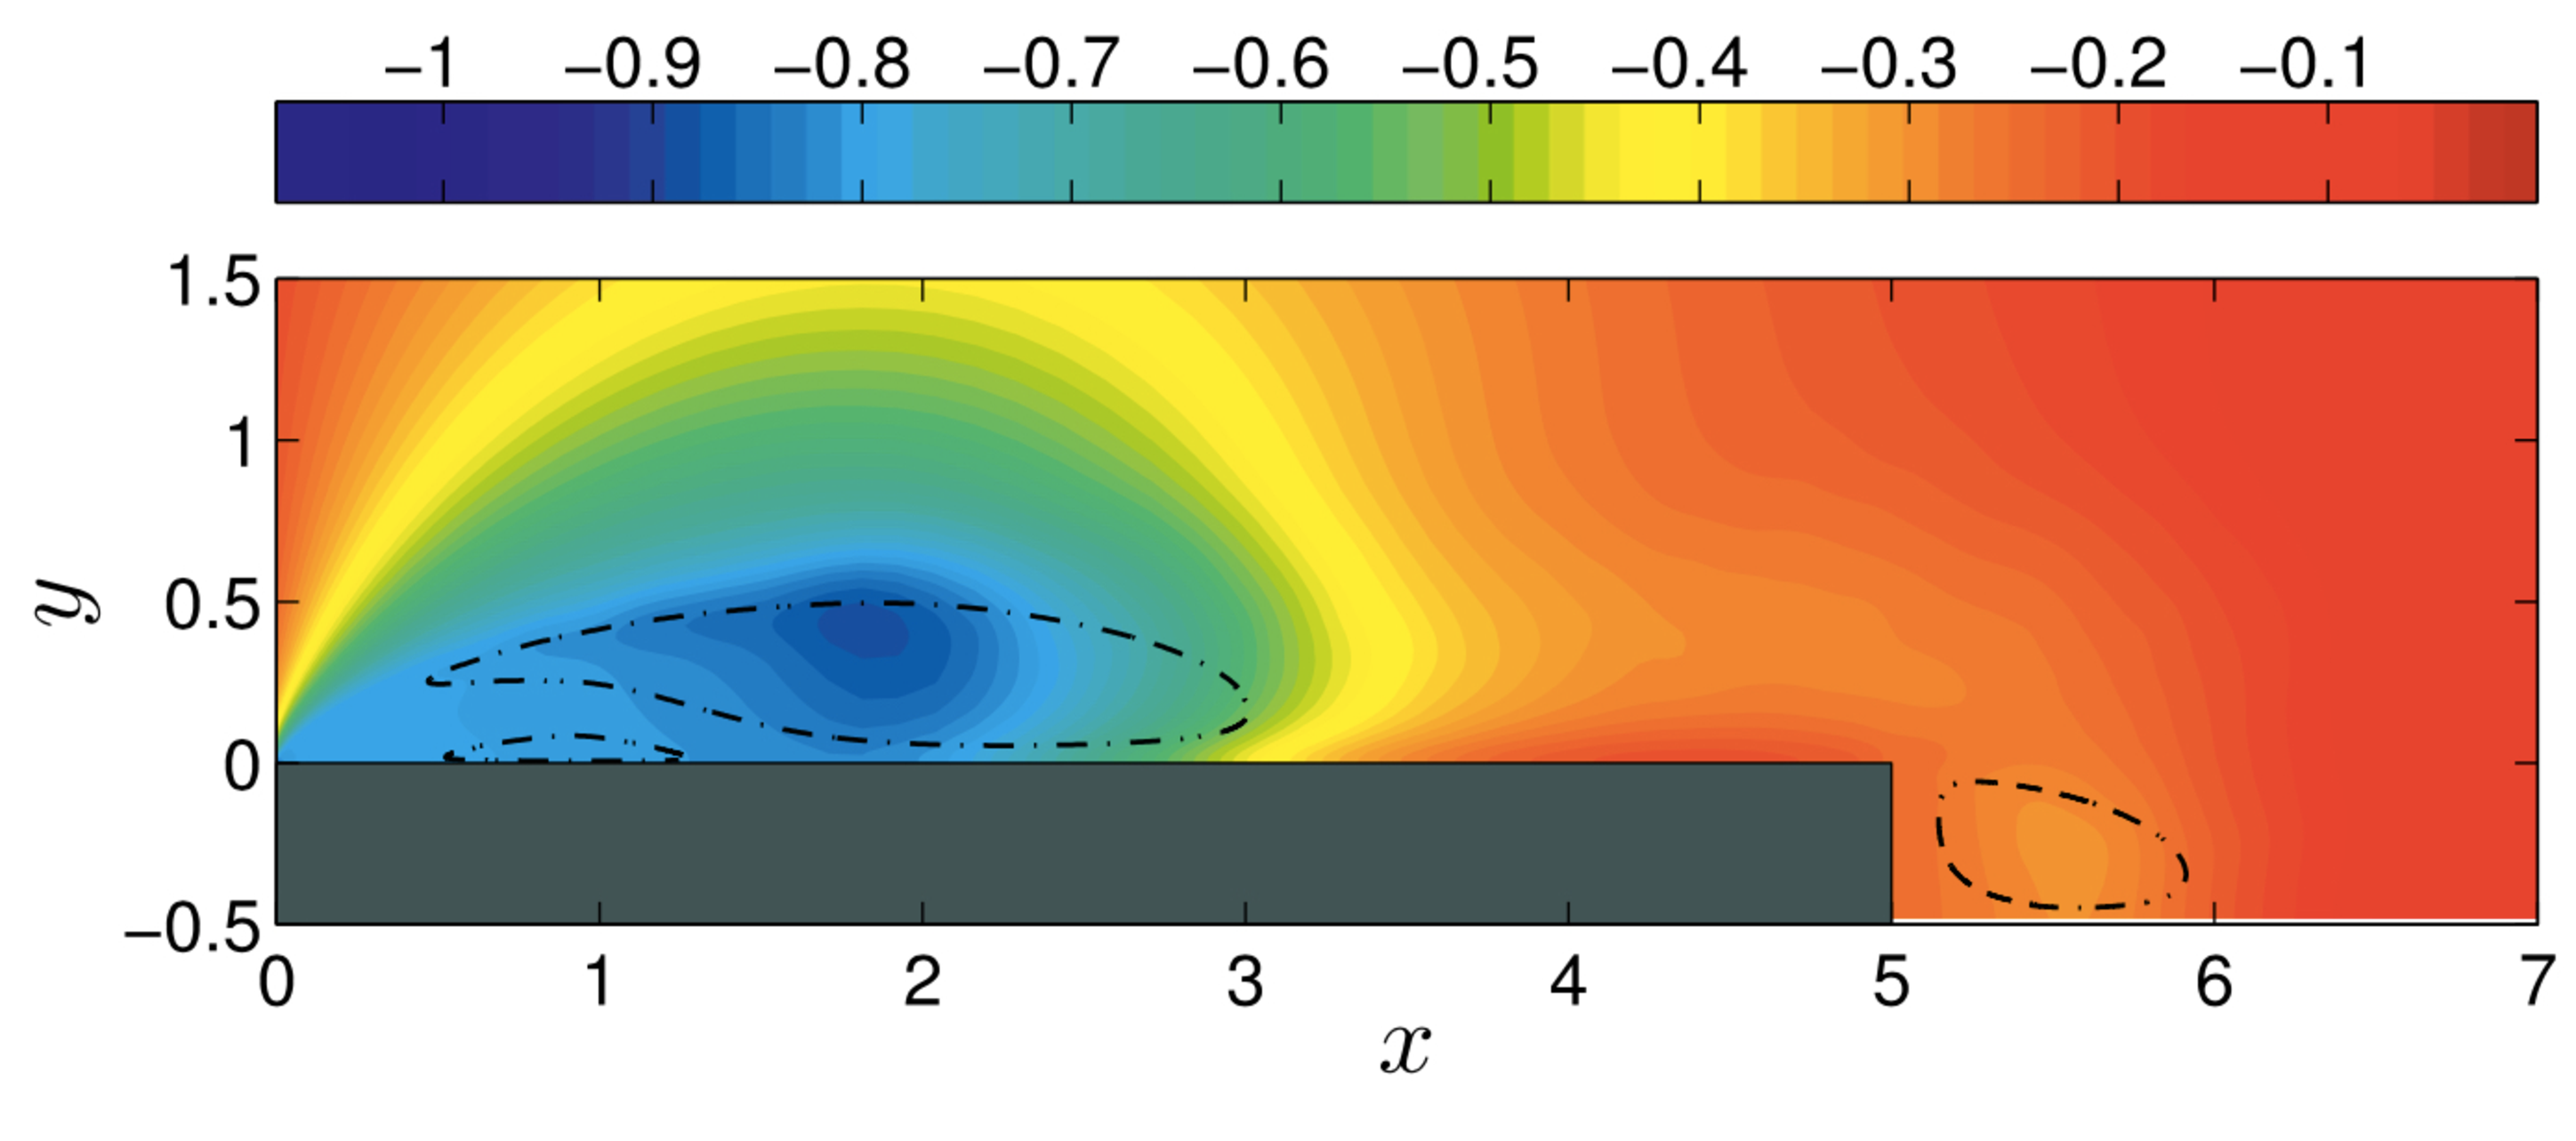
\includegraphics[width=0.45\textwidth]{Images/logan/cimarelli2018direct_pressure.pdf}
% \caption{ DNS square cylinder mean pressure distribution Re=3000 \cite{cimarelli2018direct} }
% \label{fig:dnsRectCylPressure}
% \end{center}
% \end{figure}
% %%\vspace{-2em}

% Fig. 5. Isocontours of the mean pressure field P(x,y). The dashed lines report the location of the primary vortex, secondary vortex and wake vortex.

















%%%%%%%%%%%%%%%%%%%%%%%%%%%%%%%%%%%%%%%%%%%%%%%%%%%%%%%%%%%%%%%%%%%%%%%%
\section{Conclusions}
%%%%%%%%%%%%%%%%%%%%%%%%%%%%%%%%%%%%%%%%%%%%%%%%%%%%%%%%%%%%%%%%%%%%%%%%

\textcolor{red}{\emph{LH\&FZ}}

Conclusions provide a detailed discussion of study findings. Do not introduce concepts not presented in text; do not refer to other work.



%%%%%%%%%%%%%%%%%%%%%%%%%%%%%%%%%%%%%%%%%%%%%%%%%%%%%%%%%%%%%%%%%%%%%%%%
\section*{Acknowledgments} %%%%%%%%%%%%%%%%%%%%%%%%%%%%%%%%%%%%%%%%%%%%%
%%%%%%%%%%%%%%%%%%%%%%%%%%%%%%%%%%%%%%%%%%%%%%%%%%%%%%%%%%%%%%%%%%%%%%%%

\textcolor{red}{\emph{LH\&FZ}}

%%%%%%%%%%%%%%%%%%%%%%%%%%%%%%%%%%%%%%%%%%%%%%%%%%%%%%%%%%%%%%%%%%%%%%%%
%%% BIBLIOGRAPHY %%%%%%%%%%%%%%%%%%%%%%%%%%%%%%%%%%%%%%%%%%%%%%%%%%%%%%%
%%%%%%%%%%%%%%%%%%%%%%%%%%%%%%%%%%%%%%%%%%%%%%%%%%%%%%%%%%%%%%%%%%%%%%%%

%SAMPLE CITATIONS TO SEE CITATION FORMATTING
\textcolor{red}{Example citations}

\cite{nakamura1993bluffbody}

%bibliography from .bib file, filename goes in {}
%NOTE: References must be cited with "\cite" command to appear in bibliography
%Types of Refs: article, book, conference=inproceedings, manual, mastersthesis, phdthesis, techreport, unpublished, misc (see "new-aiaa.bst")
%when you first initialize .bib file, might need to have plain text in front of \cite command to get sublime text to recognize bibliography file
\bibliography{BluffBodyTurb}

\end{document}
